% Options for packages loaded elsewhere
% Options for packages loaded elsewhere
\PassOptionsToPackage{unicode}{hyperref}
\PassOptionsToPackage{hyphens}{url}
\PassOptionsToPackage{dvipsnames,svgnames,x11names}{xcolor}
%
\documentclass[
  11pt,
  a4paper,
  twoside]{scrreprt}
\usepackage{xcolor}
\usepackage[margin=2.5cm]{geometry}
\usepackage{amsmath,amssymb}
\setcounter{secnumdepth}{5}
\usepackage{iftex}
\ifPDFTeX
  \usepackage[T1]{fontenc}
  \usepackage[utf8]{inputenc}
  \usepackage{textcomp} % provide euro and other symbols
\else % if luatex or xetex
  \usepackage{unicode-math} % this also loads fontspec
  \defaultfontfeatures{Scale=MatchLowercase}
  \defaultfontfeatures[\rmfamily]{Ligatures=TeX,Scale=1}
\fi
\usepackage{lmodern}
\ifPDFTeX\else
  % xetex/luatex font selection
\fi
% Use upquote if available, for straight quotes in verbatim environments
\IfFileExists{upquote.sty}{\usepackage{upquote}}{}
\IfFileExists{microtype.sty}{% use microtype if available
  \usepackage[]{microtype}
  \UseMicrotypeSet[protrusion]{basicmath} % disable protrusion for tt fonts
}{}
\usepackage{setspace}
\makeatletter
\@ifundefined{KOMAClassName}{% if non-KOMA class
  \IfFileExists{parskip.sty}{%
    \usepackage{parskip}
  }{% else
    \setlength{\parindent}{0pt}
    \setlength{\parskip}{6pt plus 2pt minus 1pt}}
}{% if KOMA class
  \KOMAoptions{parskip=half}}
\makeatother
% Make \paragraph and \subparagraph free-standing
\makeatletter
\ifx\paragraph\undefined\else
  \let\oldparagraph\paragraph
  \renewcommand{\paragraph}{
    \@ifstar
      \xxxParagraphStar
      \xxxParagraphNoStar
  }
  \newcommand{\xxxParagraphStar}[1]{\oldparagraph*{#1}\mbox{}}
  \newcommand{\xxxParagraphNoStar}[1]{\oldparagraph{#1}\mbox{}}
\fi
\ifx\subparagraph\undefined\else
  \let\oldsubparagraph\subparagraph
  \renewcommand{\subparagraph}{
    \@ifstar
      \xxxSubParagraphStar
      \xxxSubParagraphNoStar
  }
  \newcommand{\xxxSubParagraphStar}[1]{\oldsubparagraph*{#1}\mbox{}}
  \newcommand{\xxxSubParagraphNoStar}[1]{\oldsubparagraph{#1}\mbox{}}
\fi
\makeatother


\usepackage{longtable,booktabs,array}
\newcounter{none} % for unnumbered tables
\usepackage{calc} % for calculating minipage widths
% Correct order of tables after \paragraph or \subparagraph
\usepackage{etoolbox}
\makeatletter
\patchcmd\longtable{\par}{\if@noskipsec\mbox{}\fi\par}{}{}
\makeatother
% Allow footnotes in longtable head/foot
\IfFileExists{footnotehyper.sty}{\usepackage{footnotehyper}}{\usepackage{footnote}}
\makesavenoteenv{longtable}
\usepackage{graphicx}
\makeatletter
\newsavebox\pandoc@box
\newcommand*\pandocbounded[1]{% scales image to fit in text height/width
  \sbox\pandoc@box{#1}%
  \Gscale@div\@tempa{\textheight}{\dimexpr\ht\pandoc@box+\dp\pandoc@box\relax}%
  \Gscale@div\@tempb{\linewidth}{\wd\pandoc@box}%
  \ifdim\@tempb\p@<\@tempa\p@\let\@tempa\@tempb\fi% select the smaller of both
  \ifdim\@tempa\p@<\p@\scalebox{\@tempa}{\usebox\pandoc@box}%
  \else\usebox{\pandoc@box}%
  \fi%
}
% Set default figure placement to htbp
\def\fps@figure{htbp}
\makeatother

\ifLuaTeX
  \usepackage{luacolor}
  \usepackage[soul]{lua-ul}
\else
  \usepackage{soul}
\fi

% definitions for citeproc citations
\NewDocumentCommand\citeproctext{}{}
\NewDocumentCommand\citeproc{mm}{%
  \begingroup\def\citeproctext{#2}\cite{#1}\endgroup}
\makeatletter
 % allow citations to break across lines
 \let\@cite@ofmt\@firstofone
 % avoid brackets around text for \cite:
 \def\@biblabel#1{}
 \def\@cite#1#2{{#1\if@tempswa , #2\fi}}
\makeatother
\newlength{\cslhangindent}
\setlength{\cslhangindent}{1.5em}
\newlength{\csllabelwidth}
\setlength{\csllabelwidth}{3em}
\newenvironment{CSLReferences}[2] % #1 hanging-indent, #2 entry-spacing
 {\begin{list}{}{%
  \setlength{\itemindent}{0pt}
  \setlength{\leftmargin}{0pt}
  \setlength{\parsep}{0pt}
  % turn on hanging indent if param 1 is 1
  \ifodd #1
   \setlength{\leftmargin}{\cslhangindent}
   \setlength{\itemindent}{-1\cslhangindent}
  \fi
  % set entry spacing
  \setlength{\itemsep}{#2\baselineskip}}}
 {\end{list}}
\usepackage{calc}
\newcommand{\CSLBlock}[1]{\hfill\break\parbox[t]{\linewidth}{\strut\ignorespaces#1\strut}}
\newcommand{\CSLLeftMargin}[1]{\parbox[t]{\csllabelwidth}{\strut#1\strut}}
\newcommand{\CSLRightInline}[1]{\parbox[t]{\linewidth - \csllabelwidth}{\strut#1\strut}}
\newcommand{\CSLIndent}[1]{\hspace{\cslhangindent}#1}



\setlength{\emergencystretch}{3em} % prevent overfull lines

\providecommand{\tightlist}{%
  \setlength{\itemsep}{0pt}\setlength{\parskip}{0pt}}



 


% ------------------------------
% Header LaTeX para Quarto (PDF)
% Proyecto Docente — estilo sobrio/profesional
% ------------------------------
\typeout{=== HEADER.TEX CARGADO ===}

% Colores (necesario para \textcolor y \definecolor)
\usepackage{xcolor}
\definecolor{UAMBlue}{HTML}{002060} % azul institucional (#002060)

% Microtipografía (mejora “acabado” del texto)
\usepackage{microtype}

% Evita que LaTeX estire verticalmente las páginas
\raggedbottom

% --- Cabeceras/pies con KOMA (recomendado en Quarto PDF) ---
\usepackage[automark]{scrlayer-scrpage}
\clearpairofpagestyles

% Estilo: pequeño, cursiva, gris
\newcommand{\HeaderStyle}{\footnotesize\itshape\color{gray}}

% Cabeceras pares/impares
\lehead{\HeaderStyle Candidato: Modesto Redrejo Rodríguez} % páginas pares
\rohead{\HeaderStyle Proyecto Docente Plaza UAM2026-A1055TU}          % páginas impares

% Línea bajo cabecera (opcional)
\setheadsepline{0.3pt}

% Número de página en pie (también en páginas 'plain')
\cfoot*{\footnotesize\color{gray}\pagemark}


% ACTIVAR el estilo con cabecera
\pagestyle{scrheadings}

% IMPORTANTÍSIMO: los inicios de capítulo suelen usar 'plain' (sin cabecera).
% Forzamos que también usen scrheadings:
\renewcommand*{\chapterpagestyle}{scrheadings}

% Seguro extra: por si el template cambia el pagestyle más tarde
\AtBeginDocument{\pagestyle{scrheadings}}

% Tablas y figuras: mejor aspecto tipográfico
\usepackage{booktabs}
\usepackage{caption}
\captionsetup{
  font=small,
  labelfont=bf
}

% Evitar viudas/huérfanas (detalle de “calidad editorial”)
\widowpenalty=10000
\clubpenalty=10000


%formato tablitas
\usepackage{array}
\setlength{\arrayrulewidth}{0.3pt}
\setlength{\doublerulesep}{0pt}
%\usepackage{booktabs}
%\setlength{\lightrulewidth}{0.3pt}
%\renewcommand{\arraystretch}{1.2}


\AtBeginDocument{
  \renewcommand{\tablename}{Tabla}
  \renewcommand{\figurename}{Figura}
  \renewcommand{\chaptername}{Sección}
}

\usepackage[table]{xcolor}

% Define gris muy suave
\definecolor{lightgray}{gray}{0.95}

\usepackage{enumitem}
\setlist[itemize]{leftmargin=2em, noitemsep, topsep=0pt, partopsep=0pt, parsep=0pt}

\usepackage{longtable}
\usepackage{multirow}
\usepackage{graphicx}
\usepackage{float}
\usepackage{array} 
\usepackage[table]{xcolor}
\usepackage{hyperref}
\usepackage{fontawesome5}
\usepackage{tikz}
\usetikzlibrary{arrows.meta,positioning,babel}

%spanish
%\usepackage[spanish]{babel}

\renewcommand{\tablename}{Tabla}
\renewcommand{\figurename}{Figura}
\renewcommand{\chaptername}{Sección}

\makeatletter
\@ifpackageloaded{bookmark}{}{\usepackage{bookmark}}
\makeatother
\makeatletter
\@ifpackageloaded{caption}{}{\usepackage{caption}}
\AtBeginDocument{%
\ifdefined\contentsname
  \renewcommand*\contentsname{Table of contents}
\else
  \newcommand\contentsname{Table of contents}
\fi
\ifdefined\listfigurename
  \renewcommand*\listfigurename{Lista de figuras}
\else
  \newcommand\listfigurename{Lista de figuras}
\fi
\ifdefined\listtablename
  \renewcommand*\listtablename{Lista de tablas}
\else
  \newcommand\listtablename{Lista de tablas}
\fi
\ifdefined\figurename
  \renewcommand*\figurename{Figura}
\else
  \newcommand\figurename{Figura}
\fi
\ifdefined\tablename
  \renewcommand*\tablename{Tabla}
\else
  \newcommand\tablename{Tabla}
\fi
}
\@ifpackageloaded{float}{}{\usepackage{float}}
\floatstyle{ruled}
\@ifundefined{c@chapter}{\newfloat{codelisting}{h}{lop}}{\newfloat{codelisting}{h}{lop}[chapter]}
\floatname{codelisting}{Listing}
\newcommand*\listoflistings{\listof{codelisting}{List of Listings}}
\makeatother
\makeatletter
\usepackage{pdflscape}
\makeatother
\makeatletter
\makeatother
\makeatletter
\@ifpackageloaded{caption}{}{\usepackage{caption}}
\@ifpackageloaded{subcaption}{}{\usepackage{subcaption}}
\makeatother
\usepackage{bookmark}
\IfFileExists{xurl.sty}{\usepackage{xurl}}{} % add URL line breaks if available
\urlstyle{same}
\hypersetup{
  pdftitle={PROYECTO DOCENTE},
  pdfauthor={Modesto Redrejo Rodríguez},
  colorlinks=true,
  linkcolor={MidnightBlue},
  filecolor={Maroon},
  citecolor={MidnightBlue},
  urlcolor={MidnightBlue},
  pdfcreator={LaTeX via pandoc}}


\title{PROYECTO DOCENTE}
\author{Modesto Redrejo Rodríguez}
\date{2026-01-01}
\begin{document}

% Portada personalizada (primera página)
\begin{titlepage}
\centering
\vspace*{1cm}
\thispagestyle{empty}


\includegraphics[height=1.8cm]{images/logo_uam.pdf}\hfill
\\
\vspace{1.5cm}

\includegraphics[height=1.8cm]{images/logo_medicina.jpg}

\vspace{1.5cm}

{\Large Concurso de acceso al cuerpo de}\\[0.2cm]
{\Large Profesores Titulares de Universidad}\\[1.2cm]

{\Huge \textcolor[HTML]{002060}{\textbf{PROYECTO DOCENTE}}}\\[1.0cm]

{\LARGE \textbf{Modesto Redrejo Rodríguez}}\\[1.0cm]

{\large \textcolor[HTML]{002060}{Convocatoria:} UAM20XX-XXXXTU}\\[0.2cm]
{\small Resolución de XX de XXXX de 20XX (BOE XX/XX/20XX)}\\[0.8cm]

{\large \textcolor[HTML]{002060}{ÁREA DE CONOCIMIENTO:}}\\
{\large Bioquímica y Biología Molecular}\\[1.3cm]


\vfill
\end{titlepage}
\clearpage
\clearpage
\thispagestyle{empty}

% Cambia márgenes SOLO en esta página
\newgeometry{left=4.0cm,right=6.0cm,top=2.5cm,bottom=2.5cm}

% Ancla al inicio de página para que \vspace funcione siempre
\null

% Baja el bloque hasta ~80% de la altura útil
\vspace*{0.50\textheight}

\begin{flushleft}
\itshape
“Bioinformatics and biology communities should work together so that education of biologists in the 21st century may become as sophisticated as the computational education of physicists or economists.”\\[1.0em]
\upshape
Pavel Pevzner \& Ron Shamir (Science, 2009 - DOI: \href{https://doi.org/10.1126/science.1173876}{10.1126/science.1173876})
\end{flushleft}

% Vuelve a los márgenes normales para el resto del documento
\restoregeometry
\clearpage
\clearpage


\renewcommand*\contentsname{Contenido}
{
\setcounter{tocdepth}{2}
\tableofcontents
}
\listoffigures
\listoftables

\setstretch{1.15}
\bookmarksetup{startatroot}

\chapter{Preámbulo}\label{sec-preambulo}

Este documento describe el \textbf{Proyecto Docente} presentado por el
Dr.~Modesto Redrejo Rodríguez para optar al concurso público para la
provisión de una plaza de Profesor Titular de Universidad del área de
conocimiento ``Bioquímica y Biología Molecular'', según la Resolución de
9 de junio de 2026 de la Universidad Autónoma de Madrid, publicada en el
\href{https://www.boe.es/boe/dias/2026/06/16/}{BOE núm. 2026-146}, del
día 16 del mismo mes, con referencia UAM2026-A1055TU, que comienza
destacando las Normas Generales de aplicación:

\begin{quote}
Ley Orgánica 2/2023, de 22 de marzo de 2023, del Sistema Universitario
(en lo sucesivo, LOSU). Real Decreto 678/2023, de 18 de julio de 2023,
por el que se regula la acreditación estatal para el acceso a los
cuerpos docentes universitarios y el régimen de los concursos de acceso
a plazas de dichos cuerpos. Ley 39/2015, de 1 de octubre, de
Procedimiento Administrativo Común de las Administraciones Públicas.
Resolución de 23 de marzo de 2009 (BOCM de 27 de marzo de 2009) del
Rectorado de la Universidad Autónoma de Madrid, dictando normas para la
regulación de los concursos de acceso a plazas de Cuerpos Docentes
Universitarios, Acuerdo 14/CG de 16 de febrero de 2024 por el que se
aprueba la Normativa de concursos para el acceso a plazas de profesorado
de la UAM (BOUAM de 16 de febrero de 2024), Acuerdo 8/CG de 4 de octubre
de 2024 por el que se aprueban las bases de las convocatorias que
regirán los concursos de acceso a plazas de cuerpos docentes
universitarios (BOUAM núm. 11, de 18 de octubre de 2024), y Acuerdo
23/CG de 22 de mayo de 2026 por el que se modifica el Acuerdo 8/CG de 4
de octubre de 2024 por el que se aprueban las bases reguladoras de las
convocatorias que regirán los concursos de acceso a plazas de cuerpos
docentes universitarios; Ley de Presupuestos Generales del Estado que
fija la tasa de reposición de efectivos de las plazas de los cuerpos
docentes universitarios, siempre que por parte de las Administraciones
públicas de las que dependan se autorice la correspondiente
convocatoria. Una vez autorizado por el Consejo de Gobierno de la
Comunidad de Madrid, el Consejo de Gobierno de la Universidad Autónoma
de Madrid ha acordado la aprobación de la presente convocatoria para la
cobertura de las plazas del cuerpo docente universitario correspondiente
a la tasa de reposición de plazas de docentes universitarios, tras la
aprobación de la oferta de empleo público de la UAM del año 2025,
publicada en el «Boletín Oficial de la Comunidad de Madrid» de 4 de
agosto de 2025 y rectificada en el BOCM de 21 de agosto de 2025,
mediante concurso de acceso a las plazas del Cuerpo de funcionarios
Docentes Universitarios, que se relacionan en el anexo I de la presente
resolución al amparo del Acuerdo de Consejo de Gobierno de 28 de febrero
de 2025, y Acuerdo 23/CG de 22 de mayo de 2026 (BOUAM núm. 6, de 28 de
mayo de 2026), por el que se aprueban y resultan de aplicación las
siguientes bases.
\end{quote}

Sobre este marco normativo e institucional se inscribe el presente
Proyecto Docente, que tiene como finalidad exponer los criterios,
principios y propuestas que orientan la actividad docente del candidato
en relación con la plaza objeto de este concurso. En las bases de la
convocatoria se especifica además que en el acto de presentación los
candidatos entregarán al presidente de la comisión la siguiente
documentación por quintuplicado:

\begin{itemize}
\item
  \emph{Proyecto docente}, referido a las actividades a realizar por
  quien obtenga la plaza que figure en la convocatoria.
\item
  \emph{Proyecto investigador}, referido a las actividades a realizar
  por quien obtenga la plaza que figure en la convocatoria.
\item
  \emph{Curriculum vitae}, una de las copias debe incluir los documentos
  que acrediten o justifiquen los méritos alegados.
\end{itemize}

Este documento es el \emph{Proyecto Docente} y tiene como finalidad
definir los criterios y estrategias que orientan la actividad docente
del candidato en relación con la plaza convocada. No se limita a la
exposición de contenidos, sino que incorpora una reflexión sobre algunos
aspectos del estado actual de la disciplina, sus perspectivas de
desarrollo y las metodologías docentes que pueden resultar más adecuadas
para favorecer un aprendizaje activo y significativo.

El presente Proyecto Docente parte de las preguntas clásicas de
cualquier profesor: qué enseñar, cómo enseñar y cómo evaluar el
aprendizaje. Sin embargo, la experiencia reciente, el contexto docente
de la plaza y la influencia de los cambios tecnológicos en la
universidad aconsejan dedicar una atención especial a las metodologías
de aprendizaje activo en biociencias y, en particular, en
bioinformática. Más que ofrecer respuestas cerradas, este proyecto
pretende ordenar esa reflexión y traducirla en una propuesta docente
coherente con el entorno académico en el que se inserta.

El documento se organiza en dos grandes bloques. En primer lugar, se
presenta un análisis del contexto actual de la universidad, incluyendo
la evolución del marco legal en las últimas décadas, con especial
atención al Espacio Europeo de Educación Superior (EEES) y a la Ley
Orgánica del Sistema Universitario (LOSU, 2023). Asimismo, se describe
el entorno institucional de la Universidad Autónoma de Madrid, la
Facultad de Medicina y el Departamento de Bioquímica, detallando su
participación en la docencia de los distintos títulos oficiales de
Grado, Máster y Doctorado. En una segunda parte, se revisan algunos de
los principales enfoques metodológicos en educación superior y se
desarrolla una propuesta docente centrada en la asignatura
\emph{Bioinformática Estructural}, en el contexto del Máster en
Bioinformática y Biología Computacional, basada en metodologías de
aprendizaje activo y orientada a la mejora del proceso de
enseñanza-aprendizaje (Köpeczi-Bócz 2025; Gooblar 2019).

\newpage

\bookmarksetup{startatroot}

\chapter{Prefacio}\label{prefacio}

Según los datos más recientes de la OCDE (Organisation for Economic
Co-operation and Development 2024), la proporción de población con
educación superior en los países desarrollados se sitúa en torno al
40--45\% en la población adulta (25--64 años), con variaciones
significativas entre países.\\
España presenta valores ligeramente superiores a la media de la OCDE en
el grupo de edad de 25 a 34 años, en el que el porcentaje de población
con educación universitaria supera el 45\%, situándose por encima de
países como Alemania o Francia en ese rango de edad. Este patrón
refleja, por un lado, la expansión reciente del acceso a la educación
superior en España y, por otro, un cambio generacional relevante en el
nivel formativo de la población. De hecho, hace poco más de un siglo el
nivel de analfabetismo en España rozaba el 60\%. Al inicio de la
democracia, el nivel de alfabetización era superior al 90\%, pero el
70\% de la población abandonaba los estudios antes de completar la
educación secundaria (López Melgarejo 2019).

La evolución del sistema educativo español en las últimas décadas pone
de manifiesto el valor de las políticas públicas de acceso a la
educación y el esfuerzo sostenido de distintas generaciones por ampliar
las oportunidades formativas. El acceso a la universidad,
tradicionalmente elitista y limitado a una minoría, se ha convertido
progresivamente en una posibilidad real para gran parte de la población
española. Este cambio no solo ha transformado las trayectorias
individuales, sino que ha contribuido de manera estructural a la
configuración de una sociedad más formada y preparada para afrontar los
retos contemporáneos.

En este contexto, es necesario reconocer el papel desempeñado por
generaciones anteriores que, en condiciones más limitadas, sentaron las
bases de este progreso. En particular, la generación nacida en la
posguerra en el medio rural español afrontó importantes restricciones en
el acceso a la educación, pero contribuyó decisivamente a que las
siguientes generaciones pudieran acceder a niveles formativos más
elevados. En el plano personal, este candidato, miembro de la primera
generación de universitarios, hijo de niños de la posguerra en la España
rural, se reconoce en esa trayectoria colectiva de país. Este recorrido,
que conecta contextos sociales muy distintos en apenas dos generaciones,
ilustra el valor transformador de la educación superior, en concreto la
Universidad pública como motor del progreso social, el denominado
ascensor social (Conferencia de Rectores de las Universidades Españolas
(CRUE) 2019). Por ello, este proceso se interpreta no solo como una
evolución histórica general, sino también como una motivación adicional
para asumir con responsabilidad la función docente en el ámbito
universitario.

La elaboración de este Proyecto Docente ha supuesto una valiosa
oportunidad para reflexionar sobre la actividad docente desarrollada
hasta la fecha y sobre las perspectivas de futuro. Al mismo tiempo, ha
requerido un importante esfuerzo de recopilación y actualización de
información, tanto sobre el marco legal e institucional en el que se
inscribe la plaza como sobre los aspectos específicos de las
metodologías docentes y de la materia objeto de enseñanza. Por ello,
resulta obligado reconocer la ayuda recibida durante este proceso. La
estructura general de este Proyecto Docente, así como parte de sus
contenidos, se inspiran en proyectos docentes elaborados previamente por
profesores del Departamento de Bioquímica de la UAM, entre ellos el
Dr.~Alejandro K. Samhan, el profesor Miguel A. Fernández y, de manera
especial, la Dra. Ana Rojo, a quienes agradezco generosamente que
compartieran sus trabajos conmigo. Asimismo, el texto final se ha
beneficiado de los comentarios y sugerencias de los Dres. Mar Pérez y
Juan J. Arredondo, tanto durante la revisión de este manuscrito como a
lo largo de los últimos años.

Además, se ha empleado Microsoft Copilot como herramienta de apoyo para
la búsqueda de información, la elaboración de borradores y la generación
de tablas y esquemas. Esta herramienta se ha utilizado a través de la
licencia institucional de Microsoft 365 de la UAM, un entorno que
incorpora garantías de privacidad propias del ámbito corporativo y que
cumple con la normativa europea de protección de datos (Unión Europea
2016), manteniendo la información dentro del entorno institucional.

Con el mismo propósito de favorecer la transparencia y reproducibilidad
del proceso de elaboración, la redacción y edición del documento se han
llevado a cabo mediante el sistema Quarto integrado en RStudio. Tanto el
documento final como los archivos fuente se han depositado en un
repositorio público de GitHub (https://github.com/mredrejo/PTU2026),
bajo una licencia abierta Creative Commons BY-NC-SA\footnote{Descripción
  de la Licencia:
  \url{https://creativecommons.org/licenses/by-nc-sa/4.0/deed.es}}.

\bookmarksetup{startatroot}

\chapter{Contexto legal, institucional y académico}\label{sec-context}

Esta sección tiene como finalidad situar el presente Proyecto Docente en
el marco legal, institucional y académico que condiciona y orienta
actualmente la actividad universitaria en España. Además de
contextualizar la propuesta docente que se desarrollará en el capítulo
siguiente, esta sección se concibe como una síntesis actualizada de
referencia de consulta sobre los principales elementos normativos,
organizativos y académicos que afectan a la docencia universitaria en
España, con la intención adicional de que pueda resultar útil como base
de consulta en trabajos futuros. En este sentido, el contexto legal en
España se recoge con especial detalle en Alcubilla (2026), elaborado
inicialmente en 2016 en colaboración entre la Conferencia de Rectores de
Universidades Españolas (CRUE) y el Boletín Oficial del Estado, cuya
última modificación, a la fecha de preparación de este texto, data del 8
de mayo de 2026. A partir de este marco general, el recorrido se
organiza de forma progresiva. En primer lugar, se presentan los
principales elementos del sistema universitario español en la
Sección~\ref{sec-31}. A continuación, la Sección~\ref{sec-EEES} describe
el contexto más amplio que proporciona el Espacio Europeo de Educación
Superior (EEES o EHEA, por su nombre en inglés), que desde su puesta en
marcha con la Declaración de Bolonia de 1999 (Ministros europeos de
Educación 1999) ha constituido la referencia principal para el diseño de
la enseñanza superior en Europa. Seguidamente, la Sección~\ref{sec-UAM}
aborda el entorno institucional más próximo, formado por el sistema
universitario y el marco legal autonómico de la Comunidad de Madrid, la
Universidad Autónoma de Madrid y la Facultad de Medicina. Por último, la
Sección~\ref{sec-bq} describe el contexto docente específico del
Departamento de Bioquímica en el que se encuadra la plaza objeto de este
concurso.

\section{La universidad en España}\label{sec-31}

\subsection{Breve reseña del contexto histórico
general}\label{breve-reseuxf1a-del-contexto-histuxf3rico-general}

La universidad, como institución, tiene su origen en la Europa medieval,
a partir del desarrollo de escuelas monásticas y catedralicias que
evolucionaron hacia las primeras \emph{universitates magistrorum et
scholarium}. En España, la Universidad de Salamanca constituye uno de
los primeros ejemplos consolidados desde el siglo XIII, seguida por
otras instituciones como la de Alcalá de Henares, fundada en 1499. A lo
largo de los siglos, la universidad española ha experimentado múltiples
transformaciones, especialmente a partir del siglo XIX, con la
progresiva secularización de los estudios y la consolidación de un
sistema público orientado a la formación superior y la generación de
conocimiento.

Durante el siglo XX, la universidad española experimentó profundos
cambios asociados a los distintos contextos políticos. Tras la
aprobación de la Constitución de 1978, se reconoció el principio de
autonomía universitaria como elemento esencial del sistema, integrando
la libertad académica, la capacidad de autogobierno y la gestión de
recursos propios.

En este marco, la Ley de Reforma Universitaria de 1983 (LRU) supuso un
primer intento de modernización, orientado a incrementar la autonomía de
las universidades y mejorar la calidad docente e investigadora.
Posteriormente, la Ley Orgánica de Universidades de 2001 (LOU)
profundizó en este proceso, estableciendo un marco normativo orientado a
la mejora de la calidad, la evaluación del profesorado y la integración
en el Espacio Europeo de Educación Superior (EEES). Entre sus
principales aportaciones destacan la introducción de mecanismos de
acreditación externa del profesorado a través de la Agencia Nacional de
Evaluación de la Calidad y Acreditación (ANECA), la diversificación de
figuras docentes y la consolidación de un sistema basado en la
evaluación de la actividad académica. La LOU permitía la contratación
como personal laboral no funcionario de personal docente e investigación
(PDI) hasta un 49\% del total del mismo. Las figuras contractuales
contempladas son Profesor Ayudante, Profesor Ayudante Doctor, Profesor
Colaborador, Profesor Contratado Doctor, Profesor Asociado y Profesor
Visitante. El acceso a los cuerpos de funcionarios docentes
universitarios se rige inicialmente por un sistema de habilitación
nacional, regulado por el Gobierno, previo informe del Consejo de
Coordinación Universitaria.

La Ley Orgánica 4/2007, de 12 de abril (BOE de 13 de abril de 2007),
junto con el Real Decreto 1393/2007, de 29 de octubre, introducen
importantes actualizaciones en la LOU con el fin aumentar la autonomía
de las universidades con la introducción simultánea de mecanismos de
rendición de cuentas, así como una mayor internacionalización del
sistema universitario. Se introducen y regulan mecanismos de gobernanza
representativa y elección democrática de Rector/a. Además, se sustituyó
el sistema de habilitación nacional para el acceso a los cuerpos de PDI
funcionario por el modelo actual, pudiendo seleccionar su profesorado
entre candidatos previamente acreditados por la ANECA. Por otra parte,
se establece la ordenación de las enseñanzas universitarias oficiales
concretando la estructura de estas para adaptar los sistemas educativos
superiores al marco del Espacio Europeo de Educación Superior
(Sección~\ref{sec-EEES}), consolidando la estructura de enseñanzas en
tres ciclos sucesivos (grado, máster y doctorado).

\subsection{Ley Orgánica del Sistema Universitario español
(2023)}\label{sec-losu}

Más de dos décadas después de la LOU, los cambios sociales, tecnológicos
y económicos han impulsado la aprobación de la
\href{https://www.boe.es/buscar/act.php?id=BOE-A-2023-7500}{Ley Orgánica
2/2023, del Sistema Universitario} (LOSU, BOE 23/3/2023). Esta nueva
legislación responde a un contexto caracterizado por la digitalización
del conocimiento, la globalización, la movilidad internacional, la
transición ecológica, el feminismo y, de manera general, el avance hacia
una mayor equidad social y de género en el ámbito universitario.

A lo largo de lo que llevamos de siglo XXI se han consolidado nuevos
modelos pedagógicos que incorporan metodologías digitales en la
actividad docente. Estos modelos, junto a algunos acontecimientos
recientes como la pandemia de la CoVid-19, recualifican la educación a
distancia y obligan a potenciar el valor de la presencialidad. La
creciente importancia y significación social de la formación a lo largo
de la vida complementa la formación universitaria en la juventud. La
autonomía del aprendizaje en un entorno digital permite al profesorado
centrarse en guiar la reflexión, e innovar la experiencia docente,
complementando así el papel tradicional centrado en el control de la
memorización, habida cuenta de la disponibilidad y accesibilidad global
de la información en la sociedad del conocimiento, acrecentado si cabe
hoy día por el auge de la inteligencia artificial generativa (IAG). En
consonancia con estas transformaciones, el sistema universitario
Español, complejo y descentralizado ha protagonizado un esfuerzo de
transformación y democratización, paralelo a un incremento reciente del
número de universidades, particularmente universidades privadas. Si bien
ello ha permitido una ampliación de la oferta educativa, los requisitos
para la creación y funcionamiento de universidades han de poder asegurar
los criterios de calidad exigibles en instituciones de este tipo. La
LOSU requiere, mediante disposiciones de diverso rango, un detallado
despliegue normativo, que aún no se ha desarrollado por completo y se
extenderá previsiblemente a lo largo de varios cursos.

La LOSU introduce una visión renovada del sistema universitario como un
actor clave en la generación, transferencia y aplicación del
conocimiento en una sociedad compleja y en transformación. Entre sus
objetivos principales se encuentran la ampliación del acceso a la
educación superior, la mejora de la gobernanza universitaria, el
fortalecimiento de la investigación y la transferencia, la garantía de
la calidad institucional y la reducción de la precariedad en la carrera
académica. En este sentido, la LOSU refuerza el carácter de servicio
público de la universidad, estableciendo de forma explícita sus
funciones al servicio de la sociedad. Estas incluyen no solo la docencia
y la investigación, sino también la transferencia del conocimiento, la
innovación, la formación a lo largo de la vida y la contribución al
bienestar social, económico y ambiental. Asimismo, la ley incorpora de
manera transversal principios como la equidad, la inclusión, la
sostenibilidad, el respeto a los derechos humanos y la promoción del
pensamiento crítico.

\begin{longtable}{p{2.5cm} p{12.5cm}}

\caption{\label{tbl-funciones-losu}Funciones y principios del sistema universitario según la LOSU.}

\tabularnewline

 \\

\textbf{Nivel} & \textbf{Descripción} \\

\hline
\endfirsthead

\textbf{Nivel} & \textbf{Descripción} \\
\hline
\endhead

\hline
\endfoot

\hline
\multicolumn{2}{r}{\textit{Continúa en la página siguiente}} \\
\endfoot

\hline
\endlastfoot

\textbf{1. Función general} &
El sistema universitario garantiza el servicio público de la educación superior mediante la \textbf{docencia, la investigación y la transferencia del conocimiento}. \\

\hline

\textbf{2. Funciones del sistema universitario} &
\begin{itemize}\setlength{\itemsep}{0.2em}
\item Formación integral del estudiantado.
\item Preparación profesional.
\item Generación y transferencia del conocimiento.
\item Promoción de la innovación.
\item Contribución al bienestar social y económico.
\item Fomento del pensamiento crítico.
\item Formación a lo largo de la vida.
\item Transmisión de valores democráticos.
\end{itemize} \\

\hline

\textbf{3. Principios transversales} &
Derechos humanos, equidad, sostenibilidad, memoria democrática, lucha contra el cambio climático y Objetivos de Desarrollo Sostenible. \\

\end{longtable}

En una perspectiva más específica, los principales objetivos de la LOSU
se encuadran en la necesidad de promover desde las administraciones
públicas el acceso a la educación superior, adecuar la ordenación de las
enseñanzas universitarias, garantizar la buena gobernanza de las
instituciones universitarias, fomentar la investigación, la
transferencia y la movilidad de alumno y personal docente investigador,
garantizar la calidad de las instituciones académicas y contribuir al
fin de la precariedad laboral. En el artículo 2 de la ley, se exponen
las funciones del sistema universitario al servicio de la sociedad, que
se resumen en la Tabla~\ref{tbl-funciones-losu}.

En un contexto más general, el marco normativo estatal que regula
actualmente el sistema universitario español se articula a través de un
conjunto amplio y jerarquizado de disposiciones legales, que abordan de
manera complementaria los distintos aspectos de la actividad
universitaria. En la Tabla~\ref{tbl-legislacion-estatal-universidad} se
recoge una síntesis organizada de esta normativa, estructurada en tres
grandes bloques.

En primer lugar, la legislación básica sobre universidades, encabezada
por la LOSU, define el marco general de funcionamiento del sistema
universitario y establece sus principios fundamentales, incluyendo la
organización institucional, la gobernanza y el papel de la universidad
como servicio público. Este bloque incluye también normativa previa,
como la LOU y sus modificaciones, que han configurado históricamente el
sistema actual.

En segundo lugar, la normativa sobre acceso a los estudios
universitarios regula las condiciones de ingreso del estudiantado y los
procedimientos de admisión. En este ámbito, destaca la reciente
actualización introducida por el
\href{https://www.boe.es/buscar/act.php?id=BOE-A-2024-11858}{Real
Decreto 534/2024}, que establece un marco homogéneo para el acceso a las
enseñanzas oficiales de grado, sustituyendo a regulaciones anteriores y
reforzando los principios de igualdad, mérito y capacidad.

Finalmente, el bloque más amplio corresponde a la ordenación de las
enseñanzas universitarias y a la regulación de los títulos académicos.
Este incluye tanto normas estructurales ---como el
\href{https://www.boe.es/buscar/act.php?id=BOE-A-2021-15781}{Real
Decreto 822/2021}, que regula la organización de las enseñanzas y los
procedimientos de aseguramiento de la calidad--- como disposiciones
específicas relativas a aspectos clave del sistema, tales como el
sistema de créditos ECTS, la expedición de títulos, la homologación de
estudios extranjeros o el marco de cualificaciones. En este contexto, la
regulación de los estudios de doctorado se articula en torno al
\href{https://www.boe.es/buscar/act.php?id=BOE-A-2011-2541}{Real Decreto
99/2011}, actualizado recientemente por el
\href{https://www.boe.es/buscar/doc.php?id=BOE-A-2023-16573}{Real
Decreto 576/2023}, que adapta este tercer ciclo a las nuevas demandas
del sistema científico y universitario.

En conjunto, este entramado normativo configura un sistema complejo y en
evolución, orientado a garantizar la calidad, la transparencia y la
comparabilidad internacional de las enseñanzas universitarias, en
coherencia con los principios del Espacio Europeo de Educación Superior.

\begin{longtable}{p{5cm} p{10cm}}

\caption{\label{tbl-legislacion-estatal-universidad}Legislación estatal
en materia de universidad y estudios universitarios}

\tabularnewline

\rowcolors{2}{lightgray}{white}
 \\
\toprule
\label{tbl-legislacion-estatal-universidad} \\

\hline
\textbf{Bloque} & \textbf{Leyes o Decretos}  \\
\hline
\endfirsthead

\hline
\textbf{Nivel} & \textbf{Leyes o Decretos} \\
\hline
\endhead

\hline
\multicolumn{2}{r}{\textit{Continúa en la página siguiente}} \\
\endfoot

\hline
\endlastfoot

\textbf{Legislación básica sobre universidades (nivel estatal)} &
\begin{itemize}
\item \textbf{Real Decreto 1509/2008}, por el que se regula el Registro de Universidades, Centros y Títulos (RUCT).
\item \textbf{Ley Orgánica 2/2023}, del Sistema Universitario (LOSU).
\end{itemize}
\\ \hline

\textbf{Legislación básica sobre acceso a estudios universitarios} &
\begin{itemize}
\item \textbf{Real Decreto 534/2024}, requisitos de acceso a Grado, características básicas de la prueba de acceso y normativa básica de procedimientos de admisión.
\end{itemize}
\\ \hline

\textbf{Legislación básica sobre estudios universitarios} &
\begin{itemize}
\item \textbf{Real Decreto 1125/2003}, sistema europeo de créditos (ECTS) y sistema de calificaciones.
\item \textbf{Real Decreto 1002/2010}, expedición de títulos universitarios oficiales.
\item \textbf{Real Decreto 99/2011}, enseñanzas oficiales de doctorado.
\item \textbf{Real Decreto 22/2015}, expedición del Suplemento Europeo al Título y modificación del MECES.
\item \textbf{Real Decreto 195/2016}, expedición del Suplemento Europeo al Título de Doctor.
\item \textbf{Real Decreto 822/2021}, organización de las enseñanzas universitarias y procedimiento de aseguramiento de la calidad.
\item \textbf{Real Decreto 272/2022}, Marco Español de Cualificaciones para el Aprendizaje Permanente.
\item \textbf{Real Decreto 889/2022}, homologación, equivalencia y convalidación de títulos extranjeros.
\item \textbf{Real Decreto 576/2023}, modificación del RD 99/2011 y del RD 1002/2010.
\end{itemize}
\\ \hline

\end{longtable}

\subsection{Principales características e indicadores del sistema
universitario español
actual}\label{principales-caracteruxedsticas-e-indicadores-del-sistema-universitario-espauxf1ol-actual}

Entre las misiones y retos de la Universidad actual se encuentra la de
ofrecer a los estudiantes una formación amplia, sustentada en la
investigación, como respuesta a la creciente necesidad de conocimiento
científico y tecnológico por parte de la sociedad. En este contexto, la
investigación, la innovación y la transferencia de conocimiento deben
constituir prioridades estratégicas para los responsables académicos y
de gestión universitaria. Para dar respuesta a estas exigencias, las
universidades han reforzado sus estructuras de investigación mediante la
creación de Institutos Universitarios de Investigación y el
establecimiento de acuerdos con Organismos Públicos de Investigación
(OPIs) y otros centros de investigación en ámbitos muy diversos. Un
ejemplo claro de esta integración es la participación de las
universidades en los Institutos de Investigación Sanitaria de hospitales
acreditados por el Instituto de Salud Carlos III, así como en centros
mixtos CSIC-universidad, como el Instituto de Investigaciones Biomédicas
Sols-Morreale, en el que se integran profesores del Departamento de
Bioquímica de la UAM (Sección~\ref{sec-bq}).

Según el último informe \emph{La Universidad Española en Cifras
2023-2024} publicado por la CRUE (Hernández Armenteros and Pérez García
2025), el esfuerzo y la productividad de los investigadores españoles
han mantenido una evolución positiva en los últimos años, pese a las
limitaciones estructurales de financiación que siguen caracterizando al
sistema universitario e investigador español. En este contexto, la
producción científica del sistema universitario español continúa
destacando en el plano internacional, superando el peso relativo de la
economía española en el conjunto mundial, lo que pone de manifiesto un
elevado rendimiento en términos de generación de conocimiento. Asimismo,
la actividad investigadora se sitúa en niveles competitivos en
comparación con los países de referencia, a pesar de que el gasto en I+D
de España sigue siendo claramente inferior al de economías como Estados
Unidos, Alemania o Francia, que destinan a esta actividad porcentajes de
su PIB considerablemente superiores.

En el TOP 1000 del prestigioso ranking ARWU o \emph{Ranking de Shangai}
se mantiene una presencia significativa de universidades españolas,
mayoritariamente públicas, lo que sitúa a España entre los países con
una representación relativa destacada en este indicador. Esta posición
refleja una relación favorable entre los recursos disponibles y los
resultados obtenidos, y evidencia una notable eficiencia del sistema
universitario español en términos de rendimiento del gasto en I+D. Así,
si se considera la proporción de universidades clasificadas en el ARWU
dentro del TOP 1000 respecto al total de universidades de investigación
de cada país, España se sitúa en una posición relevante en el contexto
internacional. Al mismo tiempo, España logra situar un número
considerable de universidades en los tramos de calidad internacional,
aunque continúa mostrando una presencia limitada en los niveles de
excelencia más altos. En este sentido, resulta reseñable que según los
datos de 2024 solo una universidad española ---la Universitat de
Barcelona--- figure en el TOP 200 del ranking ARWU 2024, mientras que en
el conjunto del TOP 1000 se incluyen 36 universidades españolas, de las
cuales 35 son públicas presenciales, incluida la UAM
(Tabla~\ref{tbl-rankings-uam}), y una es privada (Universidad de
Navarra).

De acuerdo con lo anterior, el 47\% de las universidades de nuestro país
alcanzan el primer cuartil de las universidades de investigación del
mundo; 10 instituciones están clasificadas como universidades de alta
calidad en el tramo TOP 500, y otras 26 se sitúan en el tramo TOP 500 a
1000 como universidades de calidad internacional. En conjunto, estos
datos sitúan a España entre los países con una proporción más elevada de
universidades de investigación presentes en el TOP 1000 mundial.
Conviene subrayar, no obstante, que esta fortaleza se concentra sobre
todo en los tramos medios del ranking, mientras que la presencia
española en el segmento de excelencia internacional más restringido
sigue siendo reducida.

Resulta especialmente significativo analizar la relación entre el gasto
necesario en I+D y la presencia de universidades en cada uno de los
tramos del TOP 1000 considerados (Figura~\ref{fig-ranking}). Este
cociente ofrece una referencia aproximada de la eficiencia relativa de
los distintos sistemas universitarios a la hora de situar a sus
universidades en los diferentes niveles de la clasificación
internacional. Desde esta perspectiva, la figura muestra que España
presenta un comportamiento competitivo en los tramos amplios del
ranking, aunque también sugiere que, por el volumen y la intensidad de
su actividad en I+D, debería aspirar a situar alguna universidad más en
el TOP 200 del ARWU. Con todo, también debe tenerse en cuenta que la
presencia en los niveles de excelencia más altos se asocia, de forma muy
marcada, con sistemas nacionales que realizan un esfuerzo muy intenso en
I+D.

\begin{figure}

\centering{

\pandocbounded{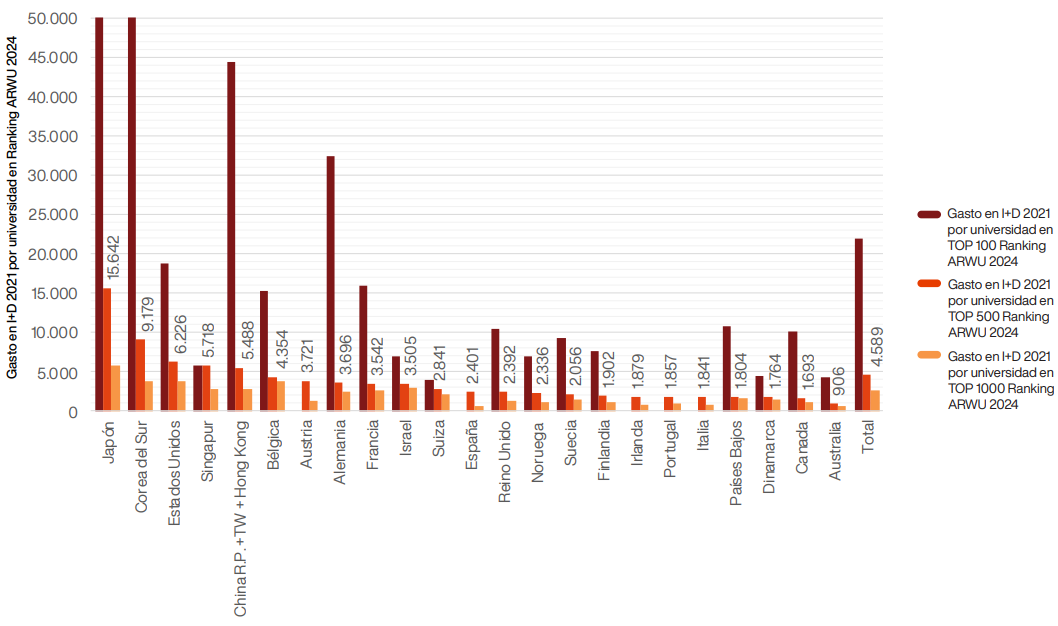
\includegraphics[keepaspectratio]{images/gasto_rankings.png}}

}

\caption{\label{fig-ranking}Gasto en I+D en 2021 por universidad situada
en el TOP 200, TOP 500 y TOP 1000 del ranking ARWU 2024 (millones de
dólares constantes de 2015) (Reproducido de Hernández Armenteros and
Pérez García 2025).}

\end{figure}%

Finalmente, en relación con la empleabilidad, las universidades
españolas continúan mostrando un desempeño favorable en el contexto
internacional. El informe destaca que la formación universitaria en
España contribuye a una reducción de la tasa de desempleo superior a la
media de la OCDE y de la Unión Europea, tanto entre la población adulta
como entre los jóvenes, consolidando el papel de la universidad como un
factor clave para la mejora de la empleabilidad. Asimismo, los
indicadores de calidad educativa sitúan al sistema universitario español
en posiciones destacadas dentro del ámbito europeo, lo que refuerza la
solidez de su modelo docente.

\section{El Espacio Europeo de Educación Superior}\label{sec-EEES}

La actual Unión Europea tuvo en sus inicios una orientación
fundamentalmente económica, centrada en conseguir la apertura de
fronteras y la creación de un espacio económico común. Sin embargo, poco
a poco se fue propiciado la convergencia de otros ámbitos, entre ellos
el educativo. El esfuerzo en educación universitaria se ha dirigido a
promover un Espacio Europeo de Educación Superior (EEES) que permita el
reconocimiento de titulaciones y asegure una formación óptima de los
estudiantes y su integración en un mercado laboral unificado.

Este espacio empezó a gestarse con la denominada \emph{Carta Magna de
las Universidades Europeas}, firmada por los rectores asistentes en
Bolonia el 18 de septiembre de 1988 con motivo del IX Centenario de la
Universidad (Ministros europeos de Educación 1999). En esta carta se
pretende dar mayor coherencia a los sistemas de educación superior en
Europa, estableciendo el EEES para facilitar la movilidad de estudiantes
y personal, hacer que la educación superior sea más inclusiva y
accesible y lograr que la educación superior en Europa sea más atractiva
y competitiva a escala mundial. Todos los países participantes acordaron
introducir un sistema de educación superior de tres ciclos, consistente
en estudios de grado, máster y doctorado; garantizar el reconocimiento
mutuo de las cualificaciones y los períodos de aprendizaje en el
extranjero completados en otras universidades y aplicar un sistema de
garantía de la calidad, a fin de reforzar la calidad y pertinencia del
aprendizaje y la enseñanza. Sin embargo, la aplicación de estas reformas
es desigual en los 48 países participantes.

Con posterioridad a la firma de esta Carta Magna, han sido variadas las
declaraciones que han contribuido a su concepción, brevemente descritas
en la Tabla~\ref{tbl-EEES}. La primera tuvo lugar en París en la
celebración del 800 aniversario de la Universidad de París, donde los
ministros de Francia, Alemania, Italia y Reino Unido realizaron una
declaración conjunta para la armonización del diseño del Sistema de
Educación Superior Europeo, en la denominada Declaración de Sorbona
(mayo de 1998). En esta declaración se asume el compromiso de la
educación superior con la sociedad y con los estudiantes en particular.
Un año después, en Bolonia (junio 1999), se realizó una declaración
conjunta de los ministros Europeos de Educación reunidos (30 países
firmantes del acuerdo). A lo largo de la década siguiente se llevaron a
cabo diversas reuniones (Praga, 2001; Berlín, 2003; Bergen 2005; Londres
2007; Lovaina 2009; Budapest y Viena-Budapest 2010) para precisar los
objetivos y mecanismos que constituirían el EEES, que además se fue
abriendo progresivamante a más países, incluidos algunos no
pertenecientes a la Unión Europea, como Suiza, Armenia, Azerbaiyán,
Ucrania, Kazajistán o Turquía, entre otros, hasta un total de 47 países.

La Tabla~\ref{tbl-EEES} muestra los principales acuerdos que forjaron el
curso de la creación e implantación del EEES. En conjunto, la evolución
del EEES muestra un desplazamiento desde una primera fase centrada en la
convergencia estructural de los sistemas universitarios hacia una etapa
posterior orientada a la calidad, la inclusión, el reconocimiento
efectivo, la empleabilidad y la defensa de los valores académicos
fundamentales.

\begin{longtable}{p{3cm} p{11.5cm}}

\caption{\label{tbl-EEES}Principales hitos en la instauración y
desarrollo del Espacio Europeo de Educación Superior (EEES). Fuente:
https://ehea.info/}

\tabularnewline

\rowcolors{2}{lightgray}{white}
 \\
\toprule
\textbf{Año y lugar} & \textbf{Hitos principales} \\
\midrule
\endfirsthead

\hline
\textbf{Año y lugar} & \textbf{Hitos principales} \\
\hline
\endhead

\hline
\endfoot

\hline
\multicolumn{2}{r}{\textit{Continúa en la página siguiente}} \\
\endfoot

\hline
\endlastfoot

1998, París &
\begin{itemize}
\item \textbf{Declaración de la Sorbona.} Francia, Alemania, Italia y Reino Unido impulsan la armonización de la arquitectura del sistema europeo de educación superior.
\item Se sientan las bases para la adopción de un sistema estructurado en ciclos y para el desarrollo posterior del EEES.
\end{itemize}
\\ \hline

1999, Bolonia &
\begin{itemize}
\item \textbf{Declaración de Bolonia.} 29 países europeos firman el acuerdo fundacional del Proceso de Bolonia.
\item Se establecen los objetivos de crear el EEES antes de 2010, promover la movilidad, el reconocimiento de titulaciones y la comparabilidad de los sistemas.
\end{itemize}
\\ \hline

2001, Praga &
\begin{itemize}
\item Los ministros de Educación revisan el proceso iniciado en Bolonia y fijan directrices y prioridades para los años siguientes, reafirmando el compromiso de constituir el EEES en 2010.
\end{itemize}
\\ \hline

2003, Graz y Berlín &
\begin{itemize}
\item En la II Convención de Instituciones de Educación Superior y en la conferencia ministerial de Berlín se refuerza la dimensión institucional del proceso y su vinculación con el Espacio Europeo de Investigación.
\item Se consolidan además diversas estructuras de seguimiento del proceso.
\end{itemize}
\\ \hline

2005, Bergen &
\begin{itemize}
\item Se subraya la importancia de implicar activamente a estudiantes, instituciones de educación superior, profesorado y empleadores.
\item Se presta especial atención al desarrollo de la investigación y de los programas de doctorado como tercer ciclo.
\end{itemize}
\\ \hline

2007, Londres &
\begin{itemize}
\item El proceso alcanza 46 países participantes.
\item Se evalúan los progresos realizados en movilidad, estructura de titulaciones, reconocimiento, marcos de cualificaciones, aprendizaje a lo largo de la vida, aseguramiento de la calidad y dimensión social.
\item Se fijan como prioridades futuras la movilidad, la dimensión social, la recogida de datos y la empleabilidad.
\end{itemize}
\\ \hline

2009, Lovaina/ Louvain-la-Neuve &
\begin{itemize}
\item Se establecen las áreas principales de trabajo para la década siguiente.
\item El proceso entra en una fase más centrada en la implantación efectiva de las reformas y en su profundización.
\end{itemize}
\\ \hline

2010, Budapest y Viena &
\begin{itemize}
\item Se celebra la conferencia aniversario de los diez años del Proceso de Bolonia.
\item Se produce el lanzamiento oficial del EEES.
\end{itemize}
\\ \hline

2012, Bucarest &
\begin{itemize}
\item El Comunicado de Bucarest se centra en consolidar el EEES en un contexto de crisis económica.
\item Se fijan como prioridades la educación superior de calidad para todos, la mejora de la empleabilidad y la movilidad.
\end{itemize}
\\ \hline

2015, Ereván &
\begin{itemize}
\item Se refuerza el seguimiento de los compromisos esenciales del proceso.
\item Se aprueba la revisión de los Criterios y Directrices para la Garantía de Calidad (ESG-2015).
\end{itemize}
\\ \hline

2018, París &
\begin{itemize}
\item Se insiste en la aplicación efectiva de los compromisos clave de Bolonia.
\item Se subrayan valores fundamentales, inclusión, empleabilidad, movilidad y calidad.
\end{itemize}
\\ \hline

2020, Roma &
\begin{itemize}
\item Visión de un EEES más inclusivo, innovador e interconectado hacia 2030.
\item Anexos sobre libertad académica, dimensión social y mejora del aprendizaje.
\end{itemize}
\\ \hline

2024, Tirana &
\begin{itemize}
\item Evaluación de avances en el 25.º aniversario del Proceso de Bolonia.
\item Reafirmación de pilares: tres ciclos, ECTS, reconocimiento y cultura de calidad.
\end{itemize}
\\ \hline

\end{longtable}

Como documento fundacional del EEES, la Declaración de Bolonia (1999) es
el documento de referencia que estableció un nuevo marco común para
modernizar y reformar la educación superior en Europa. Este marco común
se sustancia en 6 objetivos concretos:

\begin{enumerate}
\def\labelenumi{\arabic{enumi}.}
\tightlist
\item
  La adopción de un sistema único basado en dos ciclos: un ciclo de
  \emph{pre-grado} de al menos 3 años de duración y un ciclo de
  \emph{posgrado}: master o maestría y doctorado.
\item
  El establecimiento de un sistema común de Créditos, que favorezca la
  movilidad de estudiantes dentro del EEES, el ECTS (del inglés European
  Credit Transfer System, Sección~\ref{sec-ECTS}).
\item
  La adopción de un sistema fácilmente legible y comparable de
  titulaciones, mediante la implantación del denominado Suplemento de
  Título (Sección~\ref{sec-SET}), un informe con formato unificado que
  detalla las competencias adquiridas durante los distintos estudios,
  que incremente la excelencia educativa y que facilite el acceso en el
  marco del EEES.
\item
  La promoción de la cooperación europea para asegurar un nivel de
  calidad que asegure el desarrollo de criterios y metodologías
  comparables entre países.
\item
  La promoción de una necesaria dimensión europea de la Educación
  Superior, con particular énfasis en el desarrollo curricular.
\item
  La promoción de la movilidad y la desaparición de obstáculos para el
  ejercicio libre de la misma por parte de los profesores, estudiantes y
  el personal administrativo de las universidades y otras instituciones
  de enseñanza del EEES.
\end{enumerate}

Adicionalmente, entre las principales ideas transversales incluidas en
el proceso de Bolonia está la de promover una educación universitaria
más personalizada y práctica. Para ello es necesario fortalecer
fundamentalmente dos aspectos:

\begin{itemize}
\item
  Evaluación continua, con un seguimiento frecuente del trabajo y
  aprendizaje, promoviendo la programación de tutorías individuales y
  grupales y el uso de herramientas digitales.
\item
  Enseñanza práctica, con lo que se pretende fomentar la intervención
  activa del estudiante mediante la realización de ejercicios,
  proyectos, etc. individuales y en grupo que le permitan aplicar,
  desarrollar y poner a prueba sus conocimientos.
\end{itemize}

El EEES ha configurado en las últimas décadas un marco de progresiva
convergencia estructural entre sistemas universitarios europeos. Este
espacio, de naturaleza intergubernamental y más amplio que la propia
Unión Europea, ha permitido el desarrollo de instrumentos clave como el
sistema de créditos ECTS, los marcos de cualificaciones o el
reconocimiento mutuo de estudios, sentando las bases para una
cooperación educativa efectiva a escala continental. En el contexto
actual del Marco Estratégico de la UE en Educación y Formación 2030
(\emph{Education \& Training}, ET2030), el EEES no solo actúa como
soporte técnico, sino que proyecta sus objetivos hacia nuevas
dimensiones prioritarias en la política educativa europea. En
particular, los desarrollos recientes del proceso de Bolonia
(Tabla~\ref{tbl-EEES}) enfatizan la construcción de un espacio
universitario más inclusivo, innovador e interconectado, así como el
refuerzo de valores fundamentales como la libertad académica, la
integridad institucional o la participación de la comunidad
universitaria. Estas orientaciones se alinean plenamente con las
prioridades europeas de mejora de la calidad, la equidad y la
cooperación, así como con la promoción de la movilidad y la dimensión
internacional de la educación superior (European Parliamentary Research
Service 2021).

De este modo, el EEES no solo constituye actualmente la base estructural
sobre la que se apoyan las políticas de educación superior de la Unión
Europea, sino que actúa también como un marco amplio y dinámico de
innovación y de consolidación de valores compartidos, esencial para la
consecución de los objetivos definidos en ET2030.

\subsection{Implantación del Espacio Europeo de Educación Superior en la
Universidad
Española}\label{implantaciuxf3n-del-espacio-europeo-de-educaciuxf3n-superior-en-la-universidad-espauxf1ola}

El proceso de Bolonia se articuló inicialmente en España mediante el
\href{https://www.boe.es/buscar/act.php?id=BOE-A-2007-18770}{Real
Decreto 1393/2007} (BOE-A-2007-18770, de 29 de octubre), posteriormente
modificado por el
\href{https://www.boe.es/buscar/doc.php?id=BOE-A-2015-943}{Real Decreto
43/2015}, introduciendo ajustes relevantes en la estructura de las
enseñanzas oficiales.

En este marco, el diseño y desarrollo de todos los planes de estudio, de
grado y posgrado, corresponde a las universidades, en el ejercicio de su
autonomía, dentro del contexto competencial compartido entre el Estado y
las comunidades autónomas. En todo caso, dichos títulos deben someterse
a los procesos de verificación, seguimiento y acreditación realizados
por las agencias de aseguramiento de la calidad, ya sean de ámbito
nacional ---como la Agencia Nacional de Evaluación de la Calidad y
Acredictación (ANECA), organismo autónomo responsable de la evaluación
de la calidad de la educación superior--- o autonómico, según
corresponda (Sección~\ref{sec-calidad}).

Posteriormente, el
\href{https://www.boe.es/buscar/doc.php?id=BOE-A-2021-15781}{Real
Decreto 822/2021} estableció la ordenación de las enseñanzas
universitarias oficiales y el procedimiento de aseguramiento de su
calidad, constituyendo la normativa actualmente vigente. Este real
decreto mantiene la estructura básica de la oferta académica en dos
ciclos, Grado y Posgrado, con este último dividido en Máster y
Doctorado, y consolida, con carácter general, los estudios de Grado de
240 créditos ECTS, salvo en aquellos casos en los que, por directrices
específicas, la carga lectiva deba ser superior (300 o 360 créditos),
como es el caso de los grados en Medicina o Veterinaria. En
consecuencia, el modelo universitario español se articula
fundamentalmente en grados de 240 créditos, másteres de entre 60 y 120
créditos, y estudios de Doctorado, a los que se accede tras haber
superado al menos 300 créditos en las etapas formativas anteriores.

Asimismo, esta norma introdujo una modificación relevante al sustituir
la adscripción de los títulos a las tradicionales ramas de conocimiento
por los denominados ámbitos de conocimiento (Sección~\ref{sec-grado}),
en coherencia con estructuras de evaluación académica y científica
consolidadas a nivel nacional. Este cambio persiguía, por un lado,
garantizar una formación básica más transversal en los estudios de Grado
y reforzar su carácter generalista, y, por otro, promover la innovación
docente como elemento estratégico en la planificación y desarrollo de
las titulaciones.

El Real Decreto 822/2021 también reformuló los procesos de verificación,
seguimiento y acreditación de los títulos universitarios oficiales.
Sobre la base de la experiencia acumulada en el sistema universitario
español y del trabajo desarrollado por las agencias de calidad, se
plantea un rediseño procedimental orientado a mantener altos estándares
de calidad, simplificar los procesos administrativos y centrar la
evaluación en los elementos nucleares del proyecto académico que define
un título oficial de Grado, Máster o Doctorado.

Por último, como ya se ha mencionado Ley Orgánica del Sistema
Universitario (LOSU, 2023, Sección~\ref{sec-losu}) introduce asimismo
orientaciones estratégicas adicionales que refuerzan y actualizan el
marco definido por el EEES. En particular, incorpora de forma explícita
el aprendizaje permanente como función esencial de la universidad,
promueve una formación basada en competencias y orientada a la
empleabilidad, y refuerza la dimensión internacional del sistema
universitario mediante el impulso de la movilidad, los títulos conjuntos
y las alianzas europeas. Del mismo modo, se reconoce un mayor
protagonismo del estudiantado en el proceso formativo y se favorece la
apertura del sistema universitario hacia la sociedad a través de la
transferencia del conocimiento y la ciencia abierta. Estas líneas de
desarrollo, plenamente alineadas con las estrategias europeas actuales,
contribuyen a consolidar un modelo universitario más flexible, inclusivo
y conectado con los retos sociales contemporáneos.

\subsection{El Suplemento Europeo al Título}\label{sec-SET}

El Suplemento Europeo al Título (SET), regulado inicialmente por el Real
Decreto 1044/2003, de 1 de agosto, constituye un instrumento fundamental
de transparencia en el marco del Espacio Europeo de Educación Superior,
cuyo principal objetivo es facilitar la comprensibilidad y
comparabilidad de las titulaciones universitarias en Europa. Este
suplemento consiste en un modelo normalizado de información,
individualizado para cada titulado o titulada, que recoge de manera
detallada los estudios cursados, su contexto en el sistema educativo
nacional y los \emph{resultados del aprendizaje} adquiridos en términos
de competencias.

El SET se configura, por tanto, como un documento complementario al
título oficial, redactado de forma clara y estandarizada, que permite
comprender la naturaleza, el nivel, el contenido y la función de los
estudios realizados. Asimismo, se trata de un instrumento abierto que
puede integrar aprendizajes adquiridos a lo largo de la vida,
contribuyendo a la trazabilidad de los itinerarios formativos y al
reconocimiento académico y profesional de las cualificaciones obtenidas
en distintos contextos de educación superior en Europa.

\subsection{El sistema europeo de transferencia de
créditos}\label{sec-ECTS}

\begin{figure}

\centering{

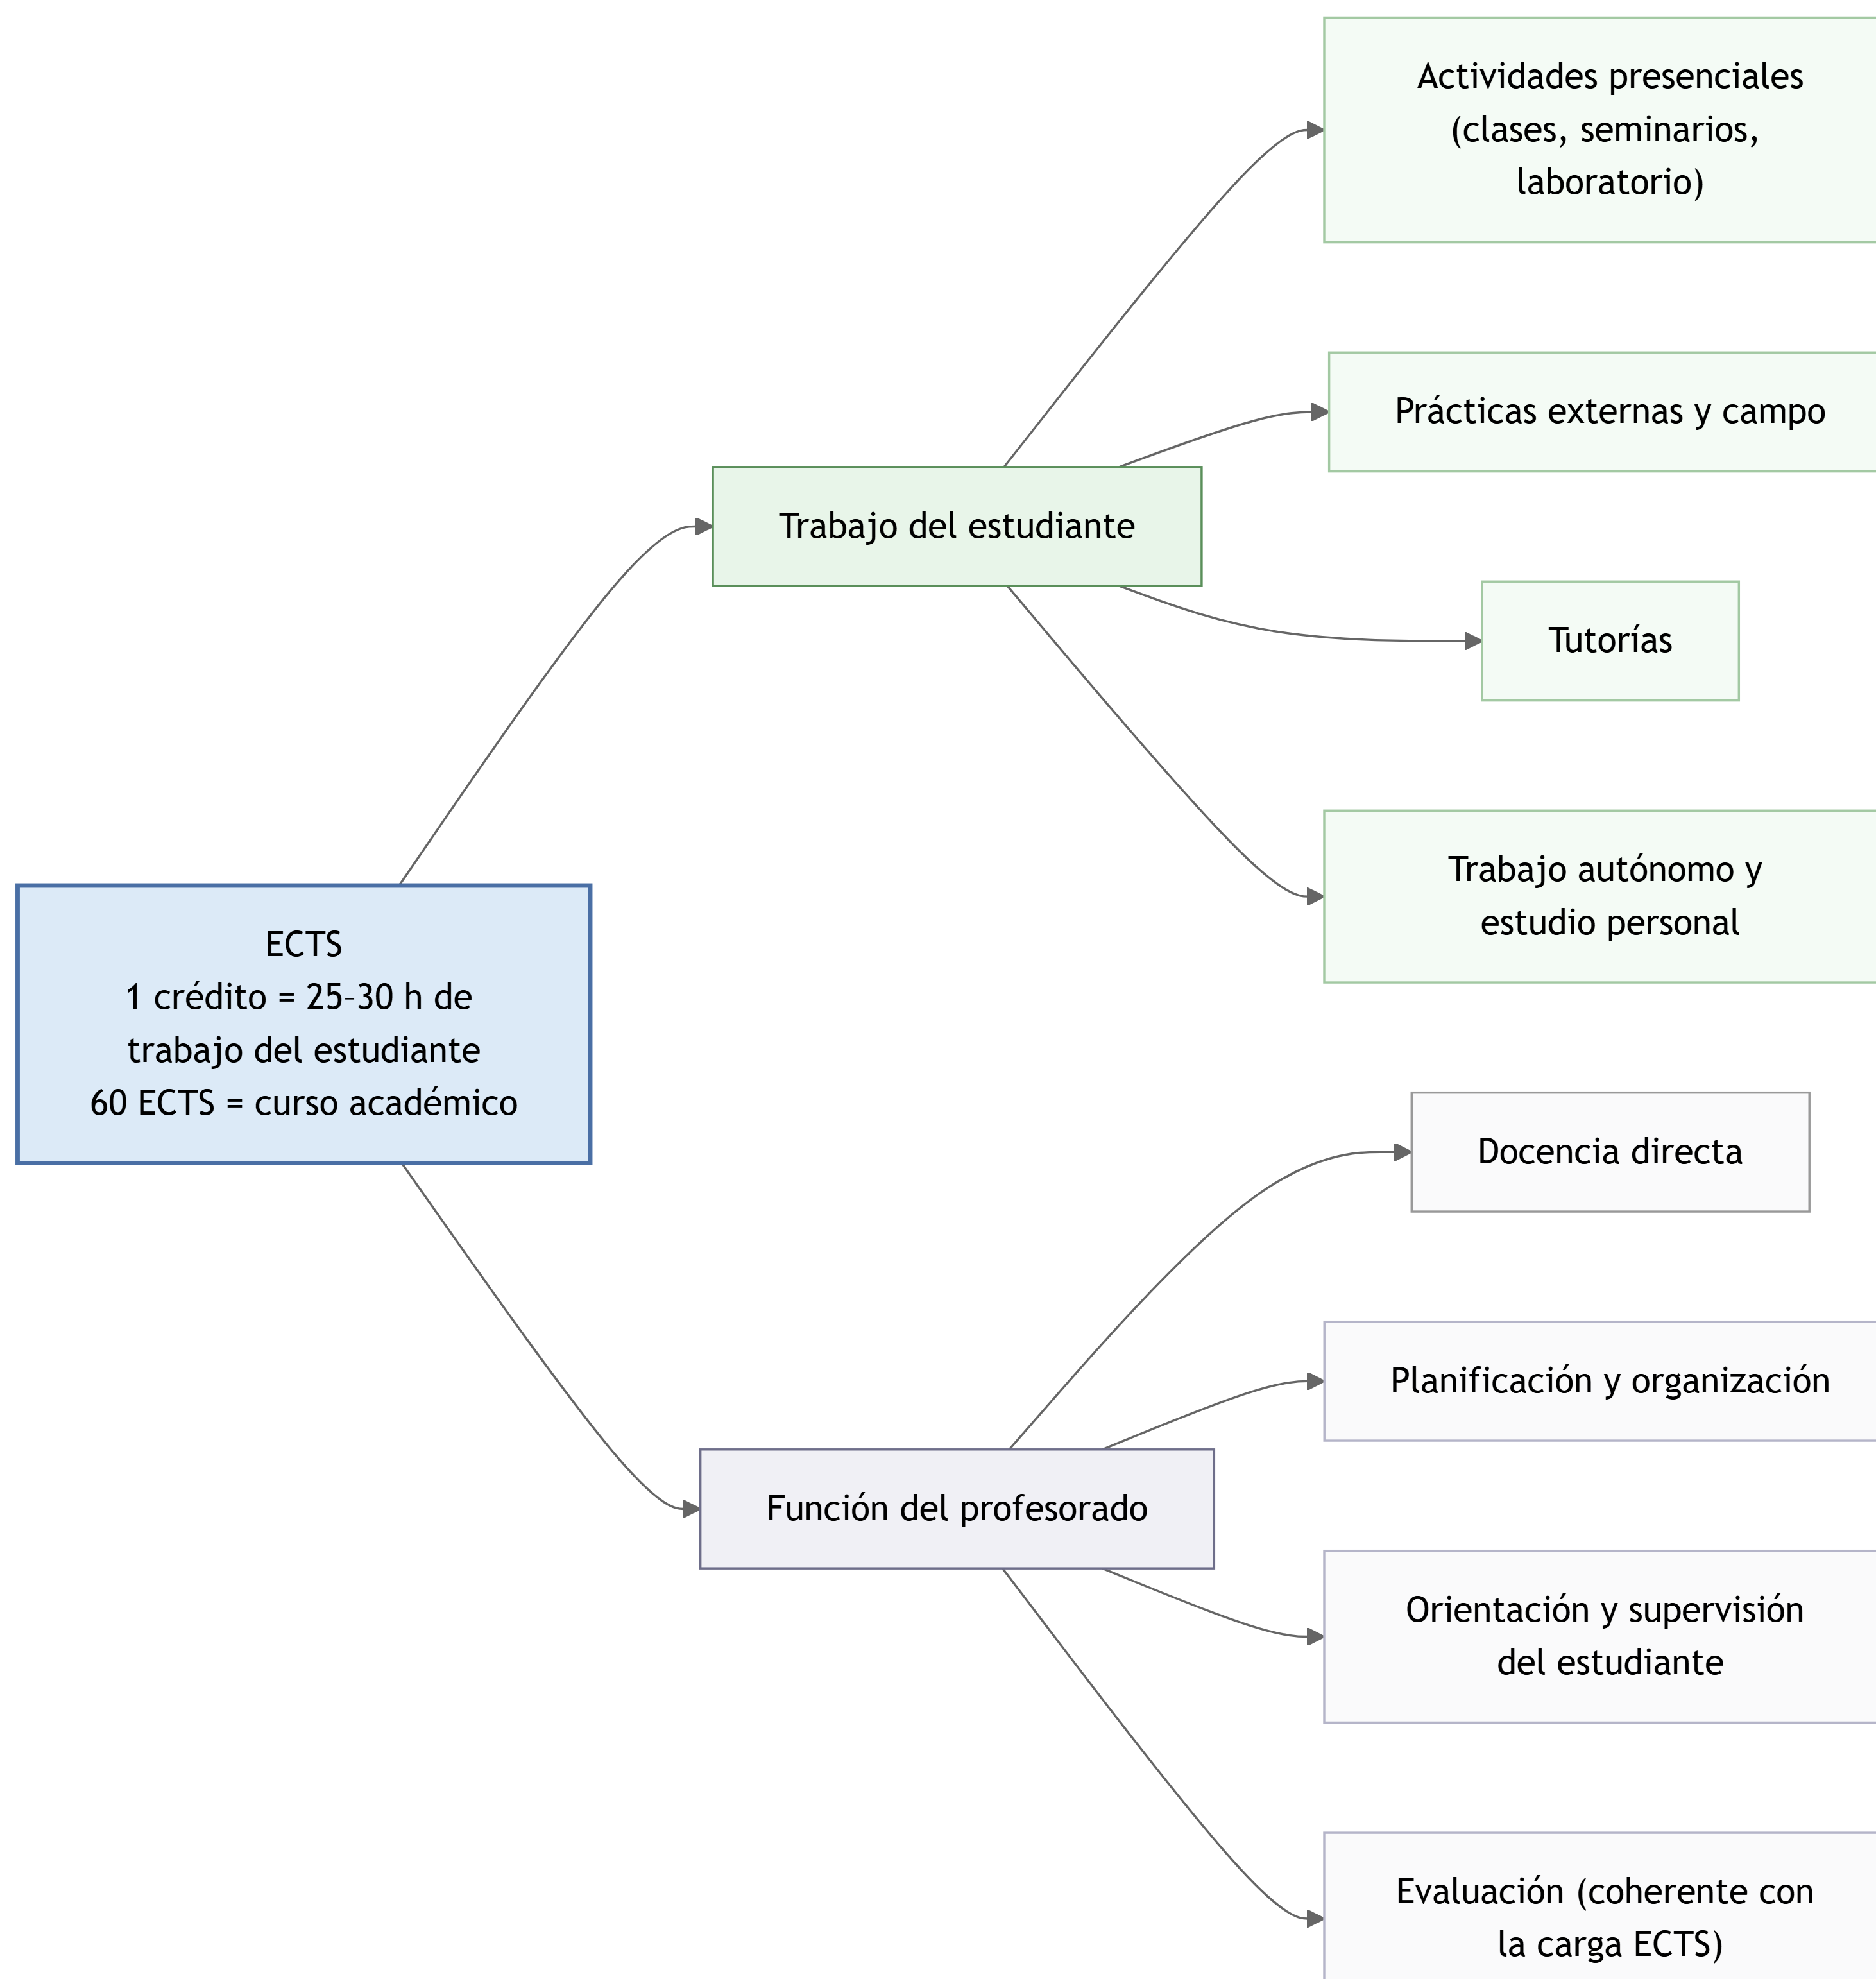
\includegraphics[width=6in,height=6.34in]{contexto_files/figure-latex/mermaid-figure-1.png}

}

\caption{\label{fig-ECTS}Descripción esquemática del ECTS.}

\end{figure}%

La generación de una unidad de medida académica para todos los
estudiantes es un objetivo fundamental para la creación del EEES, de
forma que el trabajo desarrollado por un estudiante en cualquiera de las
universidades de los estados miembros sea fácilmente reconocible en
cuanto a nivel, calidad y relevancia. Es por ello por lo que se crea el
sistema de créditos europeos, conocido como ECTS (European Credits
Transfer System), que nace y se desarrolla con los programas de
movilidad de estudiantes para dar una respuesta a la necesidad de
encontrar un sistema de equivalencias y de reconocimiento de los
estudios cursados en otros países. Su introducción en el sistema
universitario español implica importantes diferencias con respecto al
crédito vigente. Así, el crédito europeo debe quedar definido como la
unidad de valoración de la actividad académica en la que se integran las
enseñanzas teóricas y prácticas, así como otras actividades académicas
dirigidas y el volumen de trabajo que el estudiante debe realizar para
alcanzar los objetivos educativos (European Commission 2015).

Dicho de otra forma, el crédito ECTS se define a partir del volumen
total de trabajo del estudiante necesario para alcanzar los resultados
del aprendizaje, integrando tanto actividades presenciales como
autónomas y situando al profesorado como responsable del diseño,
organización y seguimiento del proceso formativo
(Figura~\ref{fig-ECTS}). En este sentido supone un cambio de paradigma
en el modelo educativo, no centrado en las horas presenciales sino
centrado en el aprendizaje.

Las programaciones de cada una de las materias que conformen el plan de
estudios de una titulación oficial deberán acogerse a esta unidad de
medida integrando en la asignación de los créditos que a cada una le
correspondan, las clases docentes teóricas y prácticas, la preparación y
realización de exámenes, horas de estudio que precisen, y los trabajos
que los alumnos deban realizar para alcanzar los objetivos formativos de
dichas materias, y todo deberá estar plasmado en la Guía Docente
disponible para los alumnos. Asimismo, en el proceso de
enseñanza-aprendizaje se enfatizan las metodologías basadas en el
autoaprendizaje del alumno (el alumno debe ``aprender a aprender'') para
favorecer la adquisición no solo de conocimientos, sino sobretodo de
habilidades y competencias.

Con respecto a las calificaciones, el Real Decreto 1125/2003 define el
sistema de calificaciones con el objetivo de facilitar su comparabilidad
en el ámbito europeo. Este establece que los resultados obtenidos por el
estudiante en cada una de las materias del plan de estudios se
expresarán en una escala numérica de 0 a 10, a la que podrá añadirse su
correspondiente calificación cualitativa:

\begin{itemize}
\tightlist
\item
  0--4,9: Suspenso (SS)
\item
  5,0--6,9: Aprobado (AP)
\item
  7,0--8,9: Notable (NT)
\item
  9,0--10: Sobresaliente (SB)
\end{itemize}

La media del expediente académico de cada estudiante se calcula como la
media ponderada de las calificaciones obtenidas, teniendo en cuenta el
número de créditos de cada asignatura:

\begin{equation}\protect\phantomsection\label{eq-media}{\bar{x} = \frac{\sum_{i=1}^{n} x_i \cdot c_i}{\sum_{i=1}^{n} c_i}}\end{equation}

Donde \(x_i\) representa la calificación obtenida en la asignatura
\(i\), mientras que \(c_i\) indica el número de créditos de dicha
asignatura. De este modo, las materias con mayor carga lectiva tienen un
peso proporcionalmente mayor en el cálculo de la nota media del
expediente académico, garantizando una evaluación global más
representativa del rendimiento del estudiante a lo largo de sus
estudios.

En conclusión, el sistema ECTS no solo permite cuantificar la carga de
trabajo del estudiante y estructurar las enseñanzas universitarias de
acuerdo con los resultados del aprendizaje, sino que también se articula
con marcos de cualificación que permiten situar dichas enseñanzas en un
contexto más amplio de comparabilidad y reconocimiento académico. En el
ámbito español, esta función la desempeña el \textbf{Marco Español de
Cualificaciones para la Educación Superior (MECES)}, que establece una
correspondencia entre los distintos niveles formativos españoles y los
estándares europeos, facilitando tanto la coherencia interna del sistema
universitario como su integración en el Espacio Europeo de Educación
Superior. De acuerdo con la legislación española
(Tabla~\ref{tbl-legislacion-estatal-universidad}), se establecen tres
ciclos denominados Grado, Máster y Doctorado, que sustancian diferentes
niveles MECES (Figura~\ref{fig-meces}).

\begin{figure}[H]

\centering{

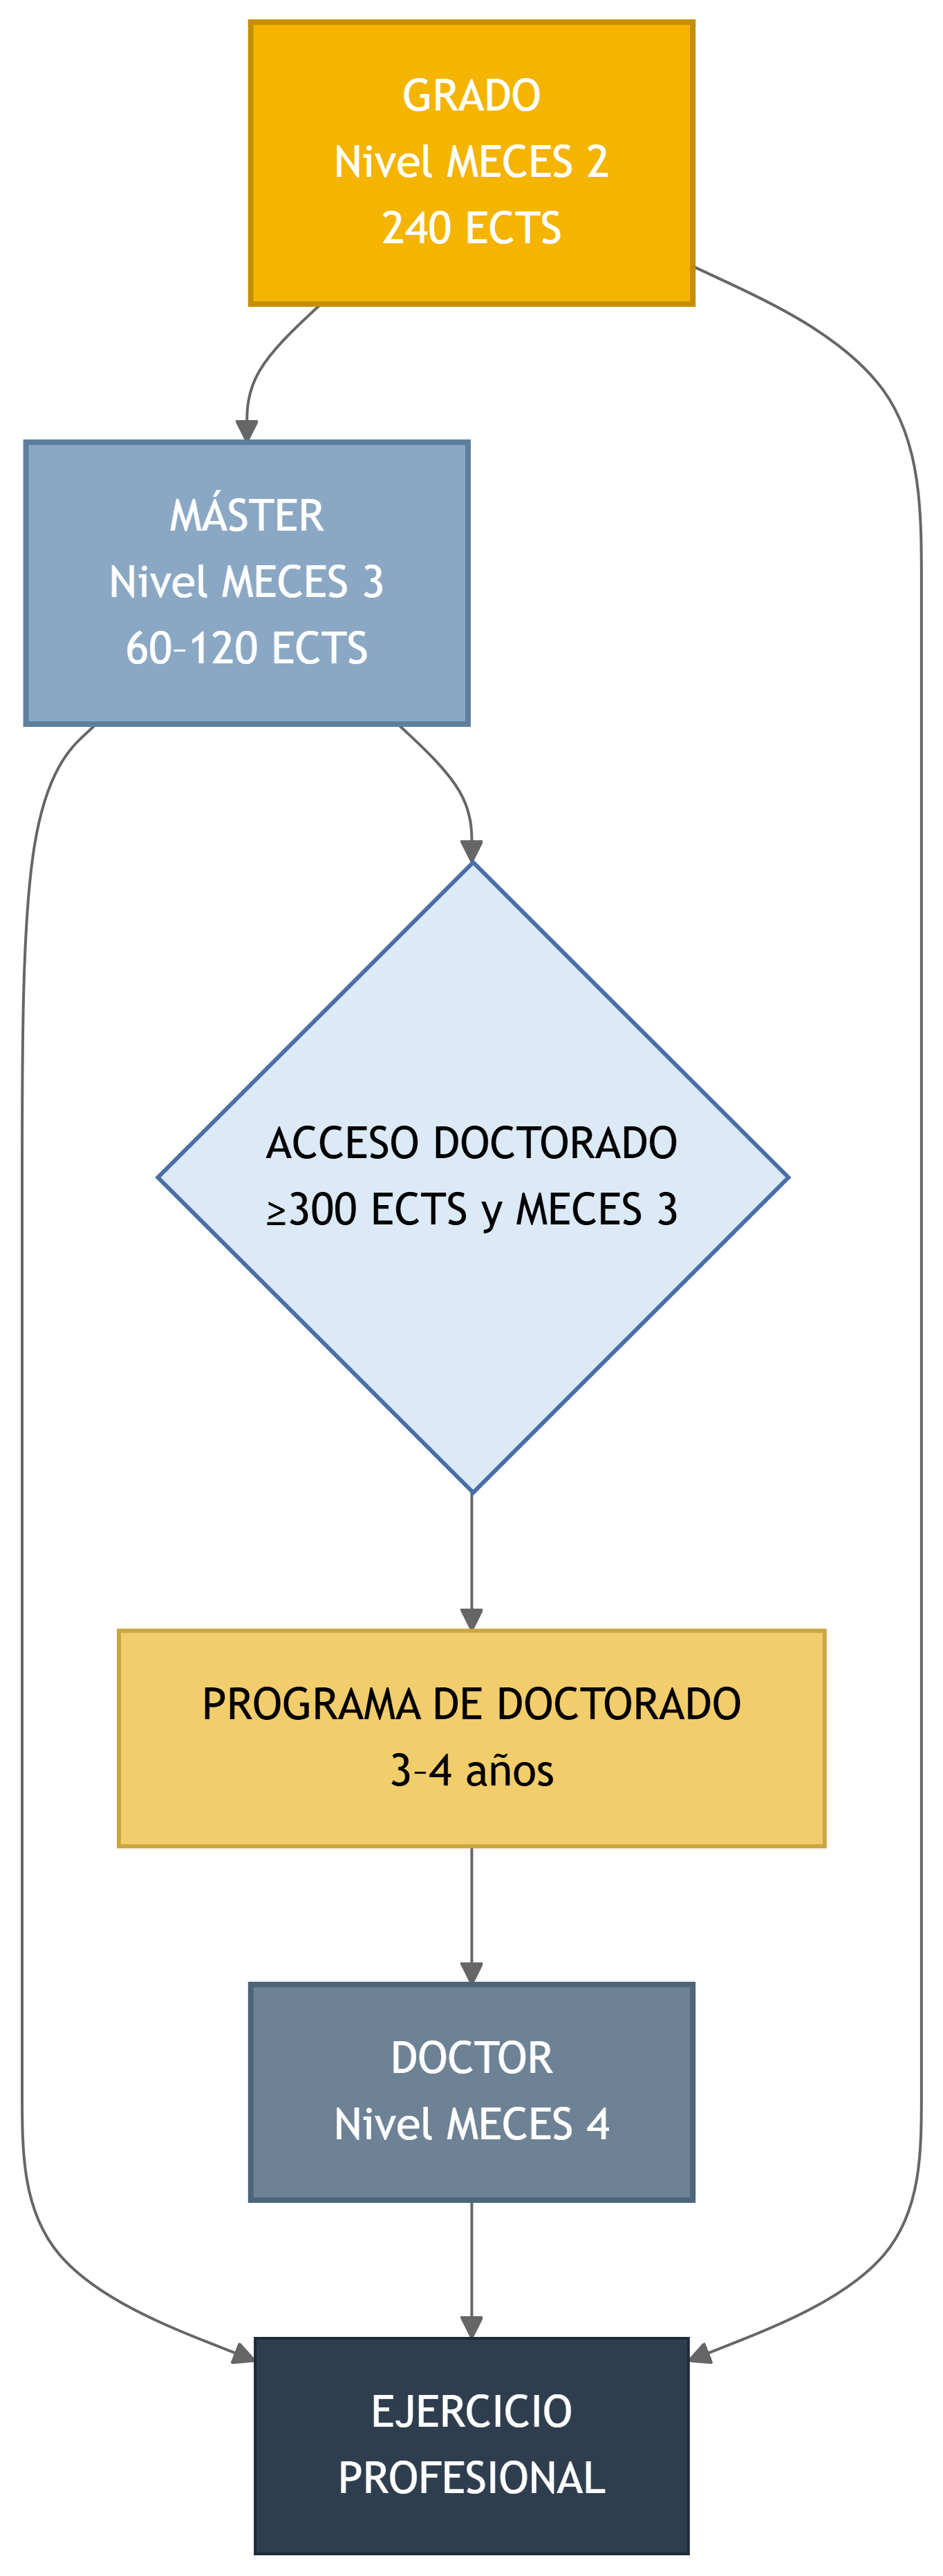
\includegraphics[width=3in,height=6.72in]{contexto_files/figure-latex/mermaid-figure-2.png}

}

\caption{\label{fig-meces}Esquema que resume la organización de los
estudios Universitarios según el EEES.}

\end{figure}%

\subsubsection{Estudios de Grado}\label{sec-grado}

Como se ha descrito en las secciones previas, la ordenación de las
enseñanzas universitarias oficiales en España ha evolucionado de forma
significativa desde la implantación del Proceso de Bolonia.
Inicialmente, dicha ordenación se articuló mediante el
\href{https://www.boe.es/buscar/act.php?id=BOE-A-2007-18770}{Real
Decreto 1393/2007}, de 29 de octubre, posteriormente modificado por el
\href{https://www.boe.es/buscar/doc.php?id=BOE-A-2015-943}{Real Decreto
43/2015}, de 2 de febrero, que introdujo mayor flexibilidad en la
duración de los estudios de Grado, permitiendo una horquilla de entre
180 y 240 créditos ECTS. No obstante, esta flexibilidad tuvo un impacto
limitado en el sistema universitario español, en el que los grados de
240 créditos se mantuvieron como modelo predominante. Con la aprobación
del \href{https://www.boe.es/buscar/act.php?id=BOE-A-2021-15781}{Real
Decreto 822/2021}, de 28 de septiembre, actualmente vigente y
desarrollado en el marco de la Ley Orgánica del Sistema Universitario
(LOSU, 2023, ver Sección~\ref{sec-losu}), se consolida de forma
generalizada la estructura de los estudios de Grado en 240 créditos
ECTS.

Este marco normativo mantiene la estructura en tres ciclos ---Grado,
Máster y Doctorado--- y consolida que los estudios de Grado tengan, con
carácter general, 240 créditos ECTS, salvo en aquellos títulos sujetos a
directrices europeas que requieran 300 o 360 créditos. Asimismo,
sustituye las tradicionales ramas de conocimiento por los actuales
ámbitos del conocimiento, que permiten una organización más flexible e
interdisciplinar de las enseñanzas.

Cabe señalar que, si bien la LOSU introduce el concepto de ámbitos del
conocimiento en el contexto de la organización del profesorado
universitario, la clasificación de los títulos oficiales continúa
rigiéndose por los ámbitos definidos en el Real Decreto 822/2021, que
sustituyó las tradicionales ramas de conocimiento por los actuales
ámbitos del conocimiento. Estos comprenden, entre otros, los siguientes
grandes campos:

\begin{itemize}
\tightlist
\item
  Actividad física y ciencias del deporte
\item
  Arquitectura, construcción, edificación y urbanismo, e ingeniería
  civil
\item
  Biología y genética
\item
  Bioquímica y biotecnología
\item
  Ciencias agrarias y tecnología de los alimentos
\item
  Ciencias biomédicas
\item
  Ciencias del comportamiento y psicología
\item
  Ciencias económicas, administración y dirección de empresas, y
  marketing
\item
  Ciencias de la educación
\item
  Ciencias medioambientales y ecología
\item
  Ciencias sociales, trabajo social y relaciones laborales
\item
  Ciencias de la Tierra
\item
  Derecho y especialidades jurídicas
\item
  Enfermería
\item
  Estudios de género y estudios feministas
\item
  Farmacia
\item
  Filología, estudios clásicos, traducción y lingüística
\item
  Física y astronomía
\item
  Fisioterapia, nutrición y otras ciencias de la salud
\item
  Historia del arte, bellas artes y expresión artística
\item
  Historia, geografía, filosofía y humanidades
\item
  Industrias culturales y audiovisuales
\end{itemize}

Si bien cada título oficial de Grado se adscribe a un único ámbito del
conocimiento, la estructura de su plan de estudios puede integrar
contenidos pertenecientes a distintos ámbitos, lo que permite una
formación interdisciplinar coherente con la naturaleza de muchas áreas
científicas. De esta forma, se permite una clasificación más precisa y
flexible de los títulos, favoreciendo la interdisciplinariedad y la
coherencia formativa de las enseñanzas universitarias.

En cuanto a la estructura académica de los estudios de Grado, estos
comprenden el conjunto de la formación teórica y práctica que el
estudiantado debe adquirir, organizada en asignaturas básicas,
obligatorias y optativas, así como en seminarios, trabajos dirigidos y
otras actividades formativas. En este sentido, la normativa establece
que la formación básica debe representar, como mínimo, el 25 \% del
total de los créditos del título, lo que equivale a 60 ECTS en los
grados de 240 créditos, garantizando una formación generalista y
transversal propia de este nivel (ver a modo de ejemplo la
Tabla~\ref{tbl-gradoBQ}). Asimismo, los planes de estudios pueden
incorporar prácticas académicas externas, entendidas como actividades
formativas realizadas por el estudiantado y supervisadas por la
universidad, cuyo objetivo es aplicar y complementar los conocimientos
adquiridos, favorecer el desarrollo de competencias profesionales,
facilitar la empleabilidad y fomentar la capacidad de emprendimiento.
Las enseñanzas de Grado concluyen con la elaboración y defensa de un
Trabajo de Fin de Grado (TFG), que se desarrolla en la fase final del
plan de estudios y está orientado a la evaluación de las competencias
asociadas al título. De acuerdo con el marco vigente, el TFG tendrá un
máximo de 24 créditos en titulaciones de 240 ECTS y deberá ser evaluado
mediante defensa pública. Por otro lado, la normativa contempla el
reconocimiento académico de créditos por la participación del
estudiantado en actividades universitarias culturales, deportivas, de
representación estudiantil, solidarias y de cooperación. Estas
actividades podrán ser objeto de reconocimiento hasta un mínimo de 6
créditos ECTS, contribuyendo a una formación integral del estudiante.
Esta previsión se encuentra en consonancia con la LOSU, que refuerza el
papel activo del estudiantado en la vida universitaria.

Finalmente, en el caso de los títulos que habiliten para el ejercicio de
profesiones reguladas, los planes de estudios deberán ajustarse a las
condiciones establecidas por el Gobierno y, en su caso, a la normativa
europea aplicable, garantizando la adquisición de las competencias
necesarias para el desempeño profesional. En este sentido, el diseño y
desarrollo de los títulos universitarios oficiales se lleva a cabo en
interacción con el entorno profesional y social, incorporando la
participación de los distintos agentes implicados. Así, junto a los
responsables académicos, resulta relevante la colaboración de
asociaciones científicas y profesionales, así como de Colegios
profesionales, cuya contribución permite alinear los contenidos
formativos con las demandas del mercado laboral, las necesidades del
ejercicio profesional y la evolución de los distintos ámbitos de
conocimiento.

En conjunto, el modelo vigente se caracteriza por una clara orientación
hacia el aprendizaje centrado en el estudiante, la formación basada en
competencias y la plena integración en el marco europeo de educación
superior, al tiempo que refuerza la relación entre la formación
universitaria y su aplicación profesional y social.

\subsubsection{Estudios de Posgrado}\label{estudios-de-posgrado}

El segundo nivel de las enseñanzas universitarias oficiales corresponde
al posgrado, al que se accede tras haber superado los estudios de Grado,
y que conduce a la obtención de los títulos de Máster Universitario y
Doctorado. Estos estudios son organizados por las universidades en el
ejercicio de su autonomía, en el marco de lo establecido por el Real
Decreto 822/2021 y la Ley Orgánica 2/2023 del Sistema Universitario
(LOSU).

En continuidad con el modelo definido en el Espacio Europeo de Educación
Superior, el posgrado se orienta tanto a la especialización académica y
profesional como a la formación investigadora avanzada, y constituye un
elemento clave para la cualificación superior del estudiantado y su
inserción en entornos profesionales altamente especializados.

\paragraph{Estudios de Máster
Universitario}\label{estudios-de-muxe1ster-universitario}

Los estudios de Máster constituyen el segundo ciclo de las enseñanzas
universitarias oficiales y tienen como finalidad proporcionar una
formación avanzada, especializada o multidisciplinar, orientada tanto a
la especialización profesional como a la iniciación en la investigación.
A diferencia de los estudios de Grado, los programas de Máster presentan
un mayor grado de flexibilidad y diversidad, permitiendo el acceso desde
distintas titulaciones previas, siempre que se garantice la adecuación
del perfil de ingreso a los objetivos formativos del programa. En este
sentido, las universidades pueden establecer complementos de formación
cuando sea necesario asegurar la adquisición de competencias previas. De
acuerdo con el marco normativo vigente, los estudios de Máster tienen
una duración comprendida entre 60 y 120 créditos ECTS, lo que equivale
generalmente a uno o dos cursos académicos. A diferencia de la
interpretación inicial de esta horquilla en el marco del Real Decreto
1393/2007, el Real Decreto 822/2021 limita la oferta actual a programas
de 60, 90 o 120 ECTS, sin configuraciones intermedias atípicas (por
ejemplo, 72 ECTS), lo que responde a la necesidad de mantener coherencia
estructural y comparabilidad dentro del sistema universitario y en el
conjunto del EEES.

Los planes de estudio de los Másteres incluyen asignaturas obligatorias
y optativas, así como, en la mayoría de los casos, un Trabajo de Fin de
Máster (TFM), de entre 6 y 30 ECTS y orientado a la evaluación de las
competencias adquiridas y, en particular, a la capacidad de integración
y aplicación de conocimientos en contextos profesionales o de
investigación. Los títulos oficiales de Máster son expedidos por el
Rector de la universidad correspondiente y en ellos figura la
denominación ``Máster Universitario en\ldots{} por la Universidad
de\ldots''.

\paragraph{Estudios de Doctorado}\label{estudios-de-doctorado}

El doctorado constituye el tercer ciclo de las enseñanzas universitarias
oficiales y tiene como finalidad principal la adquisición de las
competencias y habilidades necesarias para el desarrollo de una
investigación científica original de calidad. Estos estudios culminan
con la elaboración y defensa de una tesis doctoral, que debe aportar
resultados inéditos en el ámbito correspondiente. El marco normativo
fundamental de los estudios de doctorado se encuentra en el Real Decreto
99/2011, modificado más recientemente por el Real Decreto 576/2023, en
coherencia con la LOSU.

Con carácter general, el acceso a un programa de doctorado requiere
estar en posesión de los títulos oficiales de Grado y Máster
Universitario. Este requisito refleja la consolidación del modelo de
tres ciclos del EEES y la necesidad de haber adquirido una formación de
nivel equivalente al nivel MECES 3 (Máster) antes de iniciar la
formación investigadora avanzada.

No obstante, la normativa contempla diversas vías alternativas de
acceso, entre las que se incluyen:

\begin{itemize}
\tightlist
\item
  Estar en posesión de títulos universitarios oficiales que permitan el
  acceso a estudios de máster y haber superado al menos 300 créditos
  ECTS en el conjunto de estudios universitarios oficiales, de los
  cuales al menos 60 deberán corresponder a nivel de máster.
\item
  Estar en posesión de un título de Grado cuya duración sea de al menos
  300 ECTS conforme a normativa europea.
\item
  Haber superado con evaluación positiva al menos dos años de formación
  sanitaria especializada (MIR, BIR, FIR, etc.).
\item
  Estar en posesión de un título extranjero que acredite un nivel de
  formación equivalente al de un Máster universitario y que permita el
  acceso al doctorado en el país de origen.
\item
  Estar en posesión de titulaciones previas del sistema universitario
  anterior (DEA o suficiencia investigadora), en régimen transitorio.
\item
  Estar en posesión de otro título oficial de Doctor.
\end{itemize}

En este sentido, es importante señalar que, aunque el criterio formal de
los 300 ECTS para el acceso al doctorado sigue presente en la normativa,
el requisito general de acceso se articula a través de la posesión de un
título de Máster universitario, o de una formación equivalente a nivel
MECES 3. En la práctica, esto implica que la vía ordinaria de acceso es
la realización de estudios de máster, si bien la normativa contempla
excepciones basadas en la acreditación de una formación equivalente.

En el sistema universitario español, los estudios de doctorado se
estructuran en \emph{Programas de doctorado} cuya responsabilidad
académica recae en sus correspondientes comisiones académicas,
constituyendo estas el elemento nuclear de su organización. La normativa
vigente no impone un modelo organizativo único para estos estudios,
permitiendo a las universidades articularlos a través de Escuelas de
Doctorado u otras estructuras definidas en sus estatutos. En este
contexto, aunque muchas universidades han optado por un modelo de
escuela de doctorado única, este esquema no implica necesariamente una
organización homogénea, ya que en la práctica los programas se
estructuran en grandes áreas de conocimiento o redes temáticas. Así,
instituciones como la Universidad Autónoma de Madrid o la Universidad
Complutense concentran formalmente todos sus programas en una sola
escuela, mientras que otras, como la Universidad de Sevilla, la
Universidad de Valladolid o la Universitat Autònoma de Barcelona,
organizan su oferta doctoral en ámbitos científicos diferenciados
(ciencias, ingeniería, salud, ciencias sociales o humanidades),
configurando una estructura funcional que aproxima estos modelos a las
doctoral schools temáticas características de otros sistemas europeos.

El seguimiento del doctorando se realiza mediante planes de
investigación y evaluaciones periódicas por las comisiones académicas
del programa. La tesis doctoral constituye el eje central del doctorado
y debe consistir en un trabajo original de investigación en los ámbitos
científico, técnico, humanístico o artístico. Su defensa se realiza ante
un tribunal designado conforme a la normativa universitaria y debe ser
aprobada para la obtención del título de Doctor.

En el marco de la internacionalización del doctorado, la normativa
contempla la obtención de la \emph{Mención de Doctor Internacional}, que
reconoce la dimensión internacional de la actividad investigadora
desarrollada. Esta mención requiere, entre otros aspectos, una estancia
mínima en el extranjero, la participación de evaluadores internacionales
y la defensa parcial de la tesis en una lengua distinta de las oficiales
en España.

Esta figura sustituye en la práctica a la anterior mención de
\emph{Doctor Europeus}, actualmente en desuso, reflejando la evolución
del sistema hacia un contexto más amplio de internacionalización de la
investigación.

\subsection{Acreditación académica y evaluación de la
calidad}\label{sec-calidad}

La movilidad, el reconocimiento de estudios y la confianza mutua entre
los sistemas universitarios europeos, pilares del Espacio Europeo de
Educación Superior (EEES), requieren sistemas sólidos de garantía y
aseguramiento de la calidad. En este contexto, la calidad universitaria
se articula mediante procesos de evaluación, certificación y
acreditación orientados a la mejora continua de las enseñanzas, del
profesorado y de las instituciones.

En la actualidad, este sistema se enmarca en la Ley Orgánica 2/2023, del
Sistema Universitario (LOSU) y el Real Decreto 822/2021, y sus
principios básicos buscan reforzar los siguientes aspectos:

\begin{itemize}
\tightlist
\item
  La obligatoriedad de los sistemas internos de garantía de la calidad
\item
  La evaluación periódica de titulaciones, profesorado e instituciones
\item
  La transparencia y rendición de cuentas
\item
  La alineación con los estándares europeos (ESG, ENQA)
\end{itemize}

El sistema español de evaluación de la calidad universitaria se articula
a través de un conjunto de agencias independientes, tanto de ámbito
estatal como autonómico, en coherencia con la estructura descentralizada
del sistema universitario. A nivel estatal, la Agencia Nacional de
Evaluación de la Calidad y Acreditación (ANECA) es el organismo
responsable de la evaluación, certificación y acreditación de las
enseñanzas universitarias, así como de la coordinación general del
aseguramiento de la calidad en el Espacio Europeo de Educación Superior
(EEES). En el desarrollo de estas funciones, ANECA participa activamente
en redes internacionales de referencia, como la \emph{European
Association for Quality Assurance in Higher Education} (ENQA), el
\emph{European Quality Assurance Register} (EQAR) y la
\emph{International Network for Quality Assurance Agencies in Higher
Education} (INQAAHE), lo que garantiza la alineación del sistema español
con los estándares europeos e internacionales.

En paralelo, las comunidades autónomas disponen de agencias propias de
evaluación ---como la Fundación para el Conocimiento Madri+d en la
Comunidad de Madrid, AQU Catalunya, ACPUA en Aragón, ACSUG en Galicia o
DEVA en Andalucía--- que actúan de forma coordinada con ANECA en los
procesos de verificación, seguimiento y acreditación de títulos
oficiales. Estas agencias permiten adaptar los procedimientos de
aseguramiento de la calidad a los contextos regionales sin perder
coherencia con el marco estatal y europeo, y participan igualmente en
redes internacionales de calidad. En este contexto, ANECA estructura su
actividad en tres grandes programas, que abarcan las principales
dimensiones de la evaluación del sistema universitario, asegurando la
calidad de los estudios, el profesorado y las instituciones, tal y como
se detalla en la Tabla~\ref{tbl-aneca-programas}.

\begin{longtable}{
p{1.5cm} 
>{\centering\arraybackslash}m{2.5cm} 
m{8.5cm}
}

\caption{\label{tbl-aneca-programas}Programas de evaluación de la calidad en el sistema universitario español.}

\tabularnewline

 \\

\textbf{Tipo} & \textbf{Programa} & \textbf{Descripción} \\

\hline
\endfirsthead

\textbf{Tipo} & \textbf{Programa} & \textbf{Descripción} \\
\hline
\endhead

\hline
\endfoot


\hline
\multicolumn{3}{r}{\textit{Continúa en la página siguiente}} \\
\endfoot

\hline
\endlastfoot

\multirow{3}{1.5cm}{
\centering 
\raisebox{-0.5\totalheight}{
\rotatebox[origin=c]{90}{Profesorado}
}
}
& \parbox{2.5cm}{
\centering
\textbf{PEP} \\[0.2em]

\includegraphics[width=1cm]{images/pep.png}
}
& Evaluación para el acceso a figuras de profesorado contratado. \\

& \parbox{2.5cm}{
\centering
\textbf{ACADEMIA} \\[0.2em]

\includegraphics[width=1cm]{images/academia.png}
}
& Acreditación para el acceso a los cuerpos docentes universitarios (Profesores Titulares y Catedráticos), en el marco del RD 678/2023. \\

& \parbox{2.5cm}{
\centering
\textbf{CNEAI} \\[0.2em]

\includegraphics[width=1cm]{images/cneai.png}
}
& Evaluación de la actividad investigadora mediante sexenios. \\

\hline

\multirow{3}{1.5cm}{
\centering 
\raisebox{-1\totalheight}{
\rotatebox[origin=c]{90}{Titulos}
}
}
& \parbox{2.5cm}{
\centering
\textbf{VERIFICA} \\[0.2em]

\includegraphics[width=1cm]{images/verifica2.png}
}
& Evaluación inicial de los planes de estudio previa a su implantación. \\

& \parbox{2.5cm}{
\centering
\textbf{MONITOR} \\[0.2em]

\includegraphics[width=1cm]{images/monitor.png}
}
& Seguimiento del desarrollo e implantación del título. \\

& \parbox{2.5cm}{
\centering
\textbf{ACREDITA} \\[0.2em]

\includegraphics[width=1cm]{images/acredita.png}
}
& Renovación de la acreditación de los títulos oficiales. \\

& \parbox{2.5cm}{
\centering
\textbf{SIC} \\[0.2em]

\includegraphics[width=1cm]{images/sic.png}
}
& Programa voluntario de certificación internacional. \\

\hline

\multirow{3}{1.5cm}{
\centering 
\raisebox{-0.5\totalheight}{
\rotatebox[origin=c]{90}{Institucional}
}
}
& \parbox{2.5cm}{
\centering
\textbf{DOCENTIA} \\[0.2em]

\includegraphics[width=1cm]{images/docentia.png}
}
& Evaluación integral de la actividad docente del profesorado. \\

& \parbox{2.5cm}{
\centering
\textbf{AUDIT} \\[0.2em]

\includegraphics[width=1cm]{images/audit.png}
}
& Certificación de los sistemas internos de garantía de la calidad. \\

& \parbox{2.5cm}{
\centering
\textbf{Acreditación institucional} \\[0.2em]

\includegraphics[width=1cm]{images/acredita_institucional.png}
}
& Evaluación global de centros universitarios y reconocimiento de sus sistemas internos de calidad. \\

\end{longtable}

La LOSU impulsa especialmente la acreditación institucional como
mecanismo para simplificar procesos y reforzar la confianza en los
sistemas internos de calidad. Según el RD 822/2021, todos los títulos
oficiales de grado y posgrado deben someterse a procesos continuos de
evaluación, para garantizar la coherencia del título y su mejora
continua. En primer lugar, la \ul{verificación} consiste en la
evaluación previa del plan de estudios, realizada por las agencias de
calidad, con el fin de comprobar que el título cumple los requisitos
exigidos en términos de objetivos formativos, competencias, estructura,
recursos docentes y sistemas de evaluación. Esta verificación es
condición necesaria para la implantación del título y su inscripción en
el \emph{Registro de Universidades, Centros y Títulos} (RUCT). Una vez
implantado el título, se desarrolla su \ul{seguimiento}, proceso
continuo mediante el cual se analiza el funcionamiento real de la
titulación, atendiendo a indicadores como el rendimiento académico, la
satisfacción del estudiantado, la inserción laboral o el cumplimiento de
los objetivos formativos. Este análisis permite detectar áreas de mejora
y garantizar la calidad de la docencia de manera permanente. En tercer
lugar, la \ul{modificación} permite introducir cambios en el plan de
estudios, ya sea para adaptarlo a nuevas necesidades formativas, a
cambios normativos o a los resultados del seguimiento. Estas
modificaciones pueden ser puntuales o sustanciales, y deben ser
evaluadas conforme a los procedimientos establecidos por las agencias de
calidad. Finalmente, la \ul{acreditación} constituye una evaluación
global del título, que tiene lugar periódicamente y cuyo objetivo es
comprobar que la titulación se está desarrollando conforme a lo previsto
en la memoria de verificación, renovando así su validez oficial.

Las universidades deben disponer de sistemas formales de garantía
interna de la calidad que incluyan la recogida y análisis de
información, participación de los grupos de interés, elaboración de
informes y planes de mejora y la transparencia en los resultados. En la
UAM (Sección~\ref{sec-sigc}), estos sistemas se articulan a nivel de
centro y titulación, integrando procedimientos estratégicos, clave y de
soporte. El sistema actual incorpora mecanismos avanzados de
transparencia, como la publicación de resultados e indicadores, el
acceso a informes de evaluación y los sistemas integrados de información
universitaria (SIIU). Estos indicadores pueden ser de diverso tipo e
incluyen, por ejemplo, tasas de rendimiento y graduación, inserción
laboral, satisfacción del estudiantado, impacto social y transferencia.

En conclusión, el sistema de aseguramiento de la calidad en la
universidad española se caracteriza por su integración en el EEES, su
orientación a la mejora continua y el refuerzo de la transparencia y la
evaluación institucional, en coherencia con los principios establecidos
en la LOSU y el Real Decreto 822/2021.

\section{La Universidad Autónoma de Madrid}\label{sec-UAM}

La Universidad Autónoma de Madrid (UAM) (http://www.uam.es) es una
universidad joven, fundada en 1968 (junto con la Universidad Autónoma de
Barcelona y la Universidad del País Vasco). El complejo universitario lo
forman dos Campus (Figura~\ref{fig-campus}), el principal se encuentra
en Cantoblanco, situado a 15 Km de Madrid por la carretera M-607, en la
confluencia entre los municipios de Madrid, Alcobendas, San Sebastián de
los Reyes y Tres Cantos. Adicionalmente, un segundo campus, el Campus de
Medicina se encuentra en la zona norte de Madrid, en el Barrio del
Pilar, junto al Hospital Universitario La Paz (HULP).

\begin{figure}

\centering{

\pandocbounded{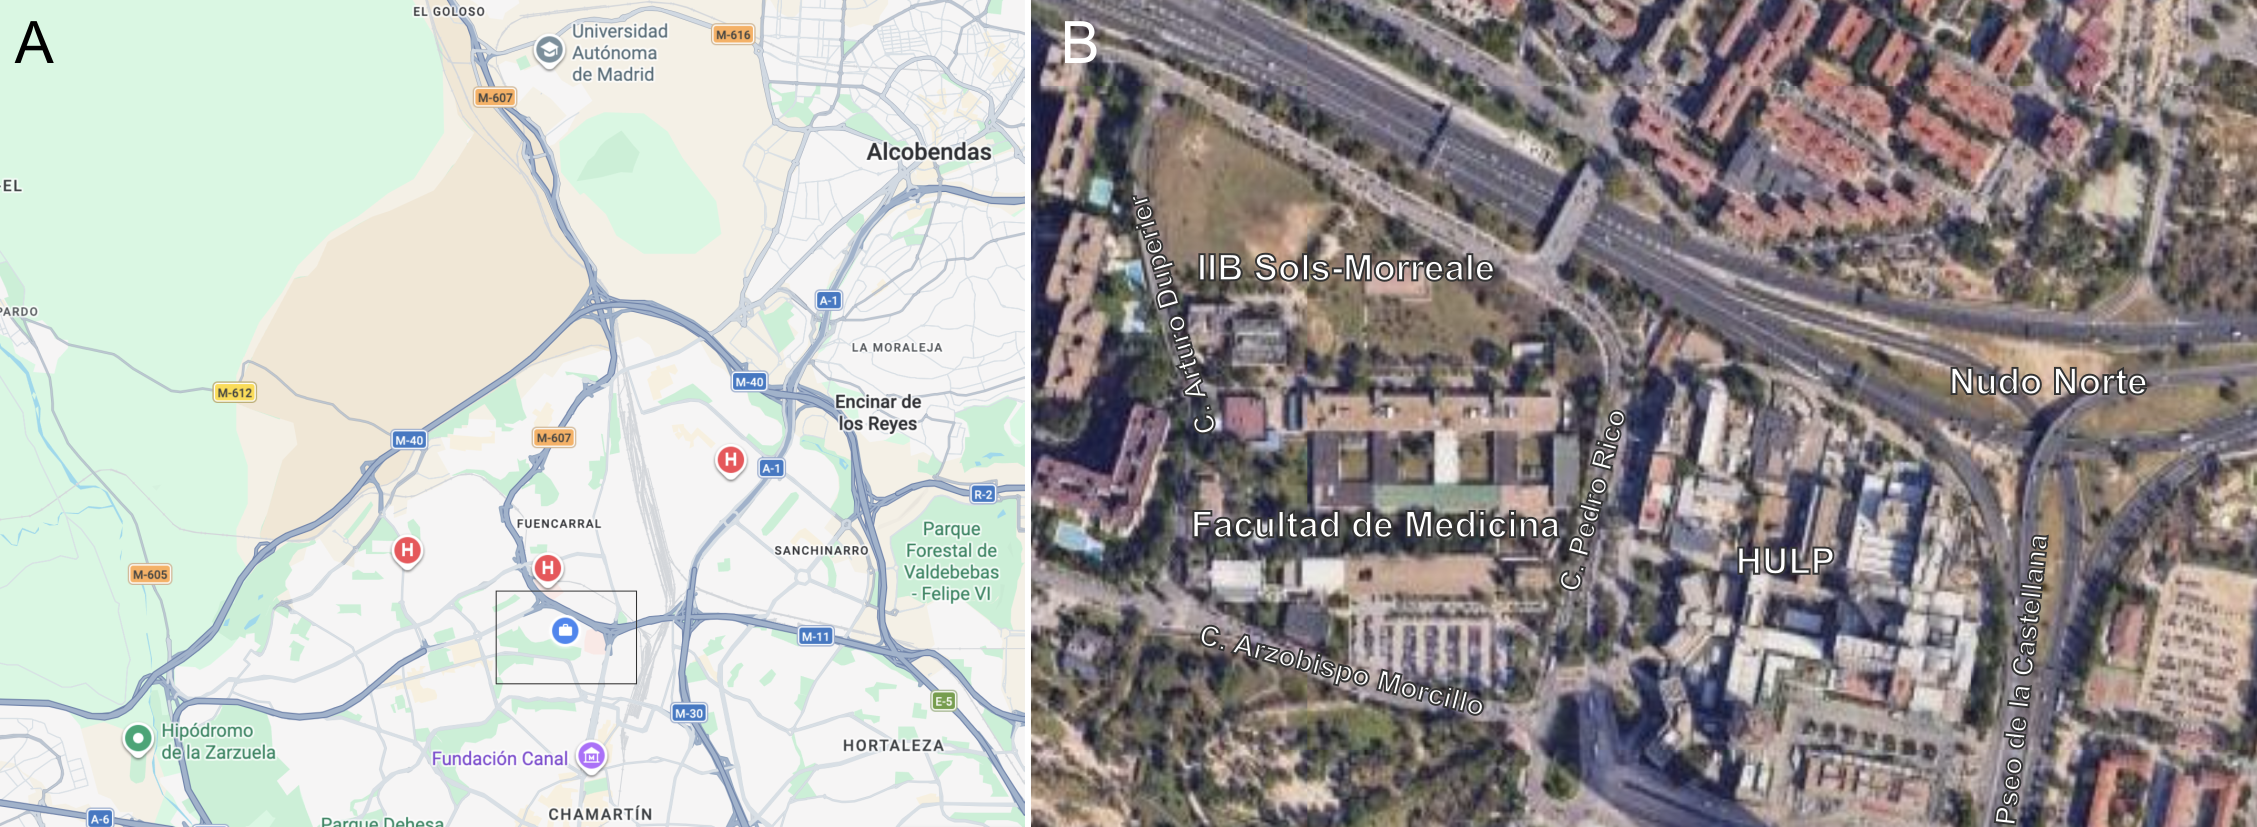
\includegraphics[keepaspectratio]{images/mapauam.png}}

}

\caption{\label{fig-campus}Mapa de la zona norte de Madrid (A) en el que
se indica la localización del Campus de Cantoblanco y (B) foto de
satélite del Campus de Medicina junto al HULP. Fuente: Google Maps}

\end{figure}%

\subsection{La UAM en el contexto regional del sistema universitario
madrileño}\label{la-uam-en-el-contexto-regional-del-sistema-universitario-madrileuxf1o}

En la Comunidad de Madrid, el marco autonómico específico en materia
universitaria sigue descansando fundamentalmente en la Ley 4/1998, de 8
de abril, de Coordinación Universitaria, aprobada pocos años después de
la asunción efectiva de competencias universitarias por parte de la
Comunidad de Madrid, en el contexto de la reforma estatutaria de 1994 y
del proceso de traspaso competencial culminado a mediados de los años
noventa. Dicha Ley creó el Consejo Universitario de la Comunidad de
Madrid y atribuyó a su Pleno, la competencia para elaborar su Reglamento
de Organización y Funcionamiento, cuya aprobación corresponde al Consejo
de Gobierno mediante Decreto. La norma fue modificada tempranamente por
la Ley 24/1998, de 21 de diciembre, y el texto consolidado del BOE
señala como última modificación el 29 de diciembre de 1998. A diferencia
de otras comunidades autónomas que sí aprobaron leyes universitarias de
carácter más amplio e integral ---por ejemplo, Cataluña, Andalucía,
Comunidad Valenciana o Castilla y León a partir de los primeros años
2000---, Madrid ha mantenido hasta la actualidad un marco normativo
relativamente limitado, centrado en la coordinación universitaria y
complementado por desarrollos reglamentarios, como el Decreto 243/1999
sobre el Reglamento de Organización y Funcionamiento del Consejo
Universitario y su posterior modificación por el Decreto 47/2005. Esta
situación ha puesto de manifiesto en distintas ocasiones la conveniencia
de revisar y actualizar la regulación autonómica, especialmente tras los
cambios introducidos por la legislación estatal universitaria posterior,
incluida la LOU y, más recientemente, la LOSU. En 2017, el Gobierno de
la Comunidad de Madrid impulsó el anteproyecto de Ley del Espacio
Madrileño de Educación Superior (LEMES), que pretendía dotar al sistema
madrileño de una regulación más completa y reforzar la docencia, la
investigación, la innovación y la transferencia de conocimiento; sin
embargo, aquel proyecto no llegó a consolidarse como ley. Más
recientemente, la Comunidad de Madrid ha trabajado en una nueva Ley de
Enseñanzas Superiores, Universidades y Ciencia (LESUC)\footnote{Borrador
  disponible en la web de la CAM:
  \url{https://www.comunidad.madrid/transparencia/sites/default/files/regulation/documents/anteproyecto_de_lemes_articulado_2017_10_11.pdf}
  (acceso verificado el 27/9/2026).}, todavía objeto de debate político
y académico, particularmente en relación con la financiación de las
universidades públicas, la autonomía universitaria y la ordenación del
conjunto del sistema de educación superior.

El sistema universitario madrileño presenta, además, una configuración
singular dentro del conjunto del Estado. En el curso 2024-2025, la
Comunidad de Madrid contaba con seis universidades públicas ---Alcalá,
Autónoma, Carlos III, Complutense, Politécnica y Rey Juan Carlos--- y
trece universidades privadas, además de la sede central de la UNED, lo
que la convierte en una de las mayores concentraciones universitarias de
España y de Europa. En los últimos años se ha producido un crecimiento
notable del sector privado universitario en la región, tanto en número
de instituciones como en volumen de estudiantes, en un contexto en el
que diversos análisis han señalado la expansión de las universidades
privadas y el debate sobre la suficiencia financiera de las
universidades públicas madrileñas. En este escenario, la Conferencia de
Rectores de las Universidades Públicas Madrileñas (CRUMA) ha adquirido
un creciente papel relevante como interlocutor colectivo de las
universidades públicas madrileñas. Su papel ha sido especialmente
visible en el acuerdo de financiación plurianual firmado en marzo de
2026 entre la Comunidad de Madrid y las seis universidades públicas,
dotado con aproximadamente 14.800 millones de euros para el periodo
2026-2031, que CRUMA valoró positivamente por aportar estabilidad,
previsibilidad y capacidad de planificación a medio plazo, aunque
subrayando la necesidad de continuidad y coherencia en el esfuerzo
financiero a largo plazo
(\href{https://www.bocm.es/boletin/CM_Orden_BOCM/2026/05/26/BOCM-20260526-5.PDF}{BOCM,
123, 26/5/2026}).

\subsection{Estadísticas y posicionamiento institucional de la
UAM}\label{estaduxedsticas-y-posicionamiento-institucional-de-la-uam}

Según el informe institucional \emph{UAM en Cifras
2024/2025}\footnote{Disponible en la web de la UAM:
  \url{https://www.uam.es/uam/media/doc/1607039905832/uam-en-cifras-2024-25.pdf}},
la Universidad Autónoma de Madrid contaba con un total de 30.826
estudiantes matriculados en enseñanzas oficiales de grado, máster y
doctorado. De ellos, 23.407 correspondían a titulaciones de grado,
mientras que 3.239 cursaban estudios de máster y 4.180 estaban
matriculados en programas de doctorado. En conjunto, la distribución por
género muestra un claro predominio de mujeres, que representan en torno
al 60\,\% del estudiantado en la mayoría de los niveles formativos. En
coherencia con esta estructura, la oferta académica de la universidad
incluía 63 titulaciones de grado, 94 titulaciones de máster y 64
programas de doctorado.

En relación con el acceso a los estudios de grado, durante el curso
2024/2025 se incorporaron 5.097 estudiantes de nuevo ingreso en centros
propios de la UAM y 833 en centros adscritos, lo que refleja una ligera
tendencia al alza respecto al curso anterior. La matrícula total en
enseñanzas de grado en centros propios alcanzó los 20.631 estudiantes,
confirmando el peso predominante de estas titulaciones dentro del
conjunto de la universidad.

En el ámbito del posgrado, la UAM mantiene una oferta consolidada y de
elevada demanda, con 3.105 estudiantes matriculados en titulaciones
oficiales de máster y 4.180 doctorandos distribuidos en sus programas de
doctorado. Estos programas continúan organizándose en las cinco grandes
ramas del conocimiento ---Artes y Humanidades, Ciencias, Ciencias de la
Salud, Ciencias Sociales y Jurídicas, e Ingeniería---, según la
estructura de la Escuela de Doctorado. Por lo que respecta a los
resultados del tercer ciclo, en el año 2024 se defendieron y aprobaron
642 tesis doctorales, lo que confirma la intensa actividad investigadora
de la institución en este nivel formativo.

En el ámbito de la investigación y la innovación, la UAM obtuvo en 2024
un total de 153 proyectos de investigación competitiva, con una
financiación asociada de 29.524.567 euros. A ello se suman 439 proyectos
de investigación contratada al amparo del artículo 60 de la LOSU, con
una financiación de 10.697.863 euros, así como 503 contratos y convenios
gestionados por la FUAM y 30 cátedras UAM-entidad, reflejando tanto la
solidez de la investigación competitiva como la intensidad de la
actividad de transferencia y colaboración institucional.

Según se detalla en la página web de la Oficina de Análisis y
Planificación de la UAM
(\url{https://www.uam.es/uam/oficina-analisis-planificacion}), la
Universidad Autónoma de Madrid mantiene un posicionamiento consolidado
en los principales rankings universitarios internacionales, situándose
de forma sostenida en rangos competitivos a nivel global y entre las
universidades mejor posicionadas de España.

Los resultados obtenidos en clasificaciones como QS, Times Higher
Education o ARWU, junto con rankings específicos por disciplinas,
empleabilidad o transferencia, reflejan una combinación de factores que
incluyen la reputación académica, la intensidad investigadora, la
proyección internacional y la calidad de la oferta formativa.

En la Tabla~\ref{tbl-rankings-uam} se recogen los valores actualizados a
julio de 2026 de algunos de los principales rankings nacionales e
internacionales. No obstante, estos datos deben interpretarse como una
referencia puntual correspondiente a las ediciones más recientes de cada
ranking, estando sujetos a variaciones anuales y diferencias
metodológicas. Por ello, su lectura más adecuada es agregada, atendiendo
a la consistencia global del posicionamiento institucional.

En este contexto, la UAM presenta una doble fortaleza: por un lado, un
sólido posicionamiento institucional; por otro, una presencia
especialmente destacada en rankings por materias, donde diversas
disciplinas se sitúan entre las mejor valoradas a nivel internacional.
Este aspecto resulta especialmente relevante, al evidenciar no solo
prestigio global, sino también excelencia académica en áreas concretas
de conocimiento, particularmente en el ámbito científico y biomédico.

\begin{landscape}

\begin{longtable}{p{3cm} p{5cm} p{8cm} p{6cm}}

\caption{\label{tbl-rankings-uam}Principales rankings universitarios recientes en los que destaca la UAM. Fuente: web de la UAM, elaboración asistida con Copilot.}

\tabularnewline

 \\

\textbf{Ranking} & \textbf{Entidad responsable y alcance} & \textbf{Qué mide principalmente} & \textbf{Posición de la UAM} \\
\hline
\endfirsthead

\textbf{Ranking} & \textbf{Entidad responsable y alcance} & \textbf{Qué mide principalmente} & \textbf{Posición de la UAM} \\
\hline
\endhead

\hline
\multicolumn{4}{r}{\textit{Continúa en la página siguiente}} \\
\endfoot

\hline
\endlastfoot

QS World University Rankings 2026
&
QS Quacquarelli Symonds. Consultora internacional; la edición 2026 clasifica 1.501 universidades y 38 españolas.
&
Combina reputación académica, reputación entre empleadores, citas por profesor, ratio profesor/estudiante, internacionalización, red internacional de investigación y sostenibilidad.
&
206 del mundo, 4.\textordfeminine{} de España y 2.\textordfeminine{} de Madrid. La UAM destaca especialmente en reputación y red internacional de investigación.
\\
\hline

QS World University Rankings: Europe 2026
&
QS Quacquarelli Symonds. Ranking europeo. La edición 2026 ordena 958 universidades de 42 países (62 españolas).
&
Incluye reputación académica y de empleabilidad, citas por publicación, publicaciones por profesor, movilidad, internacionalización y sostenibilidad.
&
71 de Europa, 3.\textordfeminine{} de España y 1.\textordfeminine{} de Madrid. La UAM destaca en reputación e internacionalización.
\\
\hline

Times Higher Education World University Rankings 2026
&
Times Higher Education (THE). Analiza 3.118 universidades a nivel mundial y 61 españolas.
&
Evalúa universidades intensivas en investigación mediante 18 indicadores agrupados en cinco pilares: enseñanza, investigación, calidad de la investigación, industria e internacionalización.
&
Rango 351--400 del mundo, 5.\textordfeminine{} de España y primera universidad de Madrid.
\\
\hline

Academic Ranking of World Universities (ARWU) 2025
&
ShanghaiRanking Consultancy. Ranking global de referencia especialmente vinculado a la investigación.
&
Premios Nobel y Medallas Fields de egresados y profesorado, investigadores altamente citados, artículos en \textit{Nature} y \textit{Science}, publicaciones indexadas y rendimiento per cápita.
&
Intervalo 301--400 mundial y puestos 3--8 de España.
\\
\hline

Best Global Universities 2025
&
U.S. News \& World Report, basado en Clarivate. La edición 2025--2026 evalúa 2.250 instituciones de 105 países.
&
Se centra en reputación investigadora y rendimiento bibliométrico: reputación global y regional, publicaciones, citas, internacionalización y artículos altamente citados.
&
281 del mundo, 114 de Europa y 5.\textordfeminine{} de España.
\\
\hline

QS World University Rankings by Subject 2026
&
QS Quacquarelli Symonds. La edición 2026 compara más de 21.000 ofertas académicas, 1.900 instituciones, 100 sistemas y 55 disciplinas.
&
Valora fortalezas disciplinares por materias y macroáreas, siendo especialmente útil para identificar áreas de excelencia académica concreta.
&
9 disciplinas en el Top 100 mundial, 26 en el Top 200 y 36 disciplinas clasificadas. La UAM es 1.\textordfeminine{} de España en Física y Astronomía, Políticas Sociales y Matemáticas.
\\
\hline

Global Employability University Ranking and Survey 2026
&
Ranking específico de empleabilidad universitaria, elaborado por "Emerging" y publicado en THE.
&
Mide la empleabilidad de los egresados a partir de la valoración directa de empleadores internacionales.
&
147 del mundo y 6.\textordfeminine{} de España.
\\
\hline

U-Ranking 2026
&
Proyecto conjunto de la Fundación BBVA y el Ivie. Compara 71 universidades españolas y más de 3.600 grados
&
Integra docencia, investigación, innovación e inserción laboral, distinguiendo entre rendimiento y volumen.
&
Por valoración global la UAM es la 6.\textordfeminine{} en España y 1.\textordfeminine{} en Madrid, destacando en Investigación e Innovación y movilidad.
\\
\hline

Ranking CYD 2026
&
Fundación CYD. La edición 2026 analiza 84 universidades y 3.909 titulaciones.
&
Ranking multidimensional que compara enseñanza y aprendizaje, I+D+i, internacionalización y contribución al desarrollo regional. 
&
4.\textordfeminine{} posición nacional por número de indicadores de alto rendimiento y 1.\textordfeminine{} en Transferencia del Conocimiento.
\\
\hline

Ranking 50 Carreras de El Mundo 2026
&
Diario \textit{El Mundo}. Clasificación nacional de orientación al estudiantado, ampliamente difundida en España. 
&
Valora los grados más demandados y las mejores facultades para cursarlos. Se elabora a partir de cerca de 30 criterios, entre ellos demanda universitaria, prácticas, relación entre estudiantes y profesorado, internacionalización, investigación y conexión con el entorno profesional.
&
La UAM sitúa 18 grados entre los más valorados del país y ocupa la 4.\textordfeminine{} posición nacional. Derecho y Física vuelven a ocupar el primer puesto, y 15/18 grados se sitúan en el Top 3.
\\
\hline

Ranking Web of Universities (WEBOMETRICS) --- edición 2025
&
Laboratorio de Cibermetría del CSIC. Ranking global centrado en la presencia e impacto web de universidades.
&
Mide visibilidad, actividad web, calidad de contenidos, prestigio internacional, apertura \textit{open access} y excelencia académica reflejada en la proyección digital de la universidad.
&
Puesto 257 a nivel mundial.
\\
\hline

\end{longtable}

\end{landscape}

\subsection{El Sistema Interno de Garantía de Calidad y la evaluación de
la docencia en la UAM}\label{sec-sigc}

Como se ha mencionado anteriormente (Sección~\ref{sec-calidad}), la
evaluación de la docencia universitaria se inscribe en un marco amplio
de aseguramiento de la calidad que ha cobrado especial relevancia en el
contexto del Espacio Europeo de Educación Superior (EEES). En el sistema
universitario Madrileño, la Fundación para el Conocimiento Madri+d es la
agencia de evaluación autonómica que participa en los procesos de
verificación, seguimiento y renovación de la acreditación de títulos
oficiales, en consonancia con los criterios establecidos por ANECA y el
EEES. La UAM ha desarrollado un sólido Sistema de Garantía Interna de
Calidad (SGIC) que constituye el eje vertebrador de todas las acciones
relacionadas con la evaluación, seguimiento y mejora continua de sus
titulaciones y de la actividad docente. Este sistema responde a los
principios recogidos en la normativa estatal y europea, integrando
mecanismos orientados a asegurar la calidad, la transparencia y la
rendición de cuentas en el ejercicio de la función docente
universitaria.

El SGIC de la UAM se caracteriza por su enfoque estructurado y
sistemático, articulado en torno a un conjunto de procedimientos
normalizados que permiten recoger, analizar y utilizar información
relevante para la toma de decisiones académicas. Estos procedimientos
abarcan tanto dimensiones globales de la calidad institucional como
aspectos específicos de cada titulación, lo que permite combinar una
visión transversal con un análisis detallado adaptado a las
particularidades de cada programa formativo. En este sentido, el sistema
contempla la evaluación de la actividad docente del profesorado, el
análisis de los resultados académicos, la valoración de la satisfacción
de los distintos grupos de interés ---especialmente el alumnado---, así
como la gestión de incidencias, reclamaciones y sugerencias.

La implantación del SGIC en la UAM se lleva a cabo principalmente a
través de las facultades y escuelas, que son responsables de su
aplicación en el ámbito de las titulaciones que gestionan. No obstante,
el sistema mantiene una coherencia institucional global, apoyándose en
plataformas comunes de gestión de la información, entre las que destaca
el Sistema Integrado de Información Universitaria (SIIU), que facilita
la recopilación y el tratamiento de datos relevantes para los procesos
de evaluación y acreditación. En este contexto, el Gabinete de Estudios
y Evaluación Institucional de la UAM desempeña un papel esencial como
órgano técnico encargado de coordinar y desarrollar las actividades
relacionadas con la evaluación de la calidad docente. Entre sus
funciones destaca la gestión y análisis de las encuestas de actividad
docente, la elaboración de informes de evaluación y la provisión de
información necesaria para los procesos de acreditación externa. Este
apoyo técnico garantiza la fiabilidad de los datos utilizados y asegura
la coherencia metodológica en los distintos procesos evaluativos.

Las encuestas de actividad docente constituyen una de las herramientas
más consolidadas en la evaluación de la calidad de la enseñanza en la
UAM. Implantadas de forma generalizada desde finales de la década de
1980 y reguladas normativamente en la actualidad, estas encuestas
permiten recoger de manera sistemática la opinión del estudiantado sobre
diferentes aspectos del proceso de enseñanza-aprendizaje, incluyendo la
organización de las asignaturas, la claridad expositiva, la adecuación
de los materiales docentes y la metodología empleada. Si bien los
resultados de estas encuestas pueden verse limitados por su
participación, constituyen el canal más útil para proporcionar
información cuantitativa a través de indicadores comparables y además
incorporar también información cualitativa mediante preguntas abiertas,
lo que permite identificar con mayor precisión fortalezas y áreas de
mejora. Los resultados de estas encuestas son accesibles a los distintos
agentes implicados, incluyendo el profesorado, los responsables
académicos y las comisiones de calidad, lo que favorece la transparencia
y la utilización efectiva de la información en los procesos de mejora.
Asimismo, estos datos se integran en los informes de seguimiento de las
titulaciones y constituyen una fuente relevante de evidencia en los
procesos de evaluación externa, como la renovación de la acreditación.

En el marco de los sistemas de garantía de calidad en la educación
superior, el programa DOCENTIA se ha consolidado como el principal
instrumento para la evaluación sistemática de la actividad docente del
profesorado universitario en España. Este procedimiento de evaluación
del profesorado forma parte de los programas promovidos por la ANECA
(Tabla~\ref{tbl-aneca-programas}) en colaboración con las agencias
autonómicas, tiene como finalidad apoyar a las universidades en el
diseño e implantación de modelos propios de evaluación docente que
favorezcan la mejora continua y el reconocimiento de la calidad en la
enseñanza.

Enmarcado en los principios del EEES, el programa DOCENTIA no se limita
a una función meramente evaluativa, sino que promueve una concepción
formativa de la evaluación docente, orientada a identificar fortalezas,
detectar áreas de mejora y estimular la innovación pedagógica. La
Universidad Autónoma de Madrid participa activamente en este programa
mediante la implantación de su modelo propio, DOCENTIA-UAM
(\url{https://www.uam.es/uam/uce/programa-docentia}), que ha sido objeto
de certificación y renovación por parte de las agencias evaluadoras, lo
que evidencia su grado de madurez y consolidación dentro del sistema
institucional de calidad. En la convocatoria más reciente de 2026, el
programa mantiene su orientación hacia la mejora de la calidad docente,
reforzando su papel como herramienta estratégica para la gestión
académica y el desarrollo profesional del profesorado. El modelo
DOCENTIA-UAM se caracteriza por una evaluación integral de la actividad
docente, que tiene en cuenta tanto las condiciones en las que esta se
desarrolla como los resultados obtenidos y el compromiso del profesorado
con la innovación y la mejora continua. De este modo, la evaluación
incorpora el análisis del encargo docente asignado, el desarrollo
efectivo del proceso de enseñanza-aprendizaje, la participación en
actividades de formación e innovación docente, así como la implicación
en tareas institucionales relacionadas con la docencia y la elaboración
de materiales didácticos. Un rasgo especialmente relevante del programa
es su enfoque basado en la utilización de múltiples fuentes de
información y en la participación de distintos agentes. La evaluación
integra datos procedentes de las encuestas de opinión del alumnado, los
autoinformes elaborados por el propio profesorado, los informes emitidos
por responsables académicos y la información disponible en las bases de
datos institucionales. Esta combinación permite obtener una visión más
completa y equilibrada de la actividad docente, superando las
limitaciones de los modelos basados en un único indicador.

El proceso de evaluación culmina con la emisión de un informe
individualizado, en el que se recoge una valoración global del desempeño
docente junto con un análisis detallado de sus distintas dimensiones.
Este informe constituye una herramienta fundamental para el desarrollo
profesional del profesorado, ya que proporciona retroalimentación
específica que puede ser utilizada para orientar la mejora de la
práctica docente. Asimismo, los resultados obtenidos tienen un impacto
relevante en los procesos de acreditación, promoción y reconocimiento
académico.

\subsection{La Facultad de Medicina de la
UAM}\label{la-facultad-de-medicina-de-la-uam}

Tras la creación de la UAM en 1968, el Ministerio de Educación y Ciencia
impulsó la creación de nuevas facultades de medicina con criterios
organizativos y docentes renovados. Con este objetivo, invitó a los
profesores José María Segovia, Diego Figuera y Vicente Rojo, procedentes
de la Clínica Puerta de Hierro, a diseñar un plan de estudios inspirado
en modelos internacionales particularmente innovadores. Según la
información recogida en el libro \emph{Cincuenta años de la Facultad de
Medicina de la UAM} (Cuervas-Mons Martínez 2018), los orígenes de la
Facultad de Medicina de la Universidad Autónoma de Madrid se remontan a
1969, aunque no fue hasta el curso 1970‑1971 cuando la Facultad pudo
iniciar sus actividades docentes en el mismo edificio en el que
actualmente se ubica.

Los objetivos planteados para la formación de los futuros médicos fueron
especialmente avanzados para su tiempo: formar médicos generales
adecuados a las necesidades sanitarias del país, dotar al estudiantado
no solo de conocimientos científicos sino también de habilidades,
actitudes y fundamentos éticos, promover un aprendizaje activo y
autónomo, coordinar la docencia entre departamentos y hospitales
vinculados y reforzar la dimensión social de la profesión médica. Este
planteamiento sentó las bases de un modelo docente centrado en la
integración entre teoría y práctica clínica, en la coordinación entre
materias y en la limitación del número de estudiantes para mantener una
adecuada proporción entre alumnado, profesorado y recursos
asistenciales.

En los años posteriores se consolidaron varios rasgos distintivos del
proyecto docente de la Facultad, entre ellos la organización coordinada
de la docencia a través de comisiones de curso, la apuesta por la
enseñanza práctica y la incorporación progresiva de la medicina de
familia y la atención primaria al proceso formativo. En este sentido, la
Facultad fue pionera en potenciar la presencia de personal docente en
centros de atención primaria mediante la creación de una unidad docente
interdepartamental vinculada a Medicina y Medicina Preventiva.

La adaptación al Espacio Europeo de Educación Superior
(Sección~\ref{sec-EEES}) supuso una nueva fase de transformación en la
Facultad. La implantación del conocido como Plan Bolonia dio lugar a la
constitución de comisiones con representación de profesorado básico y
clínico, responsables del diseño del nuevo plan de estudios y de sus
correspondientes guías docentes. A partir de entonces se reforzaron
metodologías activas como la clase teórica interactiva, los seminarios y
talleres, la resolución de problemas y casos prácticos, el trabajo en
grupo y el \emph{practicum}, con una incorporación temprana del
estudiantado a la práctica clínica real a través del laboratorio de
habilidades, del hospital y de los centros de salud. Este modelo,
todavía vigente, favorece la integración progresiva de contenidos
básicos y clínicos y una formación claramente orientada a la adquisición
de competencias.

La necesidad de evaluar adecuadamente estas competencias favoreció la
implantación del Examen Clínico Objetivo Estructurado (ECOE), una prueba
práctica estandarizada que permite valorar de forma sistemática las
competencias clínicas del estudiantado mediante la resolución de casos
en estaciones simuladas y estructuradas. Este modelo comenzó a
desarrollarse en la Facultad en el curso 2015‑2016 y, en la actualidad,
sigue constituyendo una herramienta central en la evaluación práctica
del Grado en Medicina. La web de la Facultad recoge la celebración de la
ECOE‑UAM 2026 en el Hospital Universitario La Paz, destacando su papel
como instrumento de evaluación homogénea de competencias clínicas en
escenarios simulados. En 2024\footnote{\url{https://www.uam.es/medicina/facultad/noticias/celebrada-la-prueba-ecoe-uam-2026-en-el-hospital-universitario-la-paz}}
participaron 226 estudiantes, distribuidos en 12 estaciones, con la
colaboración de más de doscientas personas en la organización.

En lo que respecta a la oferta académica actual, la Facultad de Medicina
de la UAM imparte los grados en Medicina (1.356 estudiantes), Enfermería
(616), Ingeniería Biomédica (186), Nutrición Humana y Dietética (152) y
Bioquímica (302), así como el Doble Grado en Nutrición Humana y
Dietética y Ciencia y Tecnología de los Alimentos (92), tal como recoge
la propia web del centro. Según los datos del portal institucional UAM
Data Public (UAMData, \url{https://datapublic.uam.es/}) para el curso
2023/2024, estas cifras de matrícula reflejan el peso y la diversidad de
la oferta formativa de la Facultad, con una distribución equilibrada
entre titulaciones consolidadas y otras de carácter más especializado.

La Facultad se organiza actualmente en doce departamentos, que
generalmente se denominan como \emph{departamentos básicos} (Anatomía,
Histología y Neurociencia, Farmacología y Terapéutica, Fisiología,
Medicina, Medicina Preventiva y Salud Pública y Microbiología, y
Bioquímica) y departamentos \emph{clínicos} (Anatomía Patológica,
Cirugía, Enfermería, Obstetricia y Ginecología, Pediatría, y
Psiquiatría). Además, la información institucional del centro destaca la
existencia de cinco unidades clínicas docentes vinculadas a los
hospitales universitarios La Paz, Puerta de Hierro Majadahonda, La
Princesa, Niño Jesús y Fundación Jiménez Díaz, así como una amplia red
de 24 centros de salud de atención primaria asociados a la docencia
clínica.

En el ámbito del posgrado oficial, la Facultad oferta actualmente cinco
másteres oficiales: Máster Universitario en Bioinformática y Biología
Computacional, Biomedicina Molecular, Epidemiología, Investigación
Farmacológica y el recientemente aprobado Máster en Neurociencia y
Neurotecnología. Además, profesorado de la Facultad actúa como
co-coordinador o forma parte de la Comisión Académica de otros másteres
impartidos en la Facultad de Ciencias, como los de Biomoléculas y
Dinámica Celular, Biotecnología y Microbiología. Asimismo, la Facultad
mantiene seis programas de doctorado verificados conforme al Real
Decreto 99/2011. En el curso 2024/2025, el Programa de Doctorado en
Medicina y Cirugía contó con 660 doctorandos matriculados y 102 tesis
leídas; el de Biociencias Moleculares, con 752 doctorandos y 120 tesis
leídas; el de Epidemiología y Salud Pública, con 58 doctorandos y 7
tesis leídas; el de Neurociencia, con 63 doctorandos y 13 tesis leídas;
el de Farmacología y Fisiología, con 74 doctorandos y 10 tesis leídas; y
el de Microbiología, con 122 doctorandos y 16 tesis leídas.

La Facultad de Medicina se integra, además, en un entorno biosanitario e
investigador de excepcional densidad, que incluye el Instituto de
Investigaciones Biomédicas ``Sols‑Morreale'' (centro mixto UAM‑CSIC), el
Instituto Teófilo Hernando de I+D del Medicamento y la proximidad a
centros de referencia adscritos al Instituto de Salud Carlos III, como
el CNIO y el CNIC. La combinación de docencia, práctica clínica e
investigación traslacional sigue siendo, en consecuencia, uno de los
rasgos definitorios del campus de Medicina de la UAM.

Uno de los pilares esenciales de la Facultad es la Política de Calidad,
integrada dentro de la estrategia general de calidad de la UAM
(Sección~\ref{sec-sigc}). Su propósito principal es fomentar la
excelencia académica en todas sus titulaciones, tanto de grado como de
máster, con el objetivo de afianzar una cultura institucional orientada
a la calidad. Se busca que todas las personas implicadas en los procesos
de enseñanza y aprendizaje adopten esta filosofía en su día a día, y que
los futuros egresados desarrollen una sólida conciencia sobre la
importancia de la calidad, valor que será apreciado tanto por los
empleadores como por la sociedad en su conjunto. En este marco de
actuación, la Facultad de Medicina ha implementado un Sistema Interno de
Garantía de Calidad (SIGC) que permite aplicar procedimientos de mejora
continua mediante la evaluación sistemática de los procesos, el análisis
de los resultados obtenidos y el cumplimiento de los Objetivos de
Calidad establecidos por el Centro. Como parte de este compromiso con la
mejora constante, tanto la Política como los Objetivos de Calidad son
revisados periódicamente. Tras su análisis por los órganos colegiados y
los grupos de interés correspondientes, se realizarán las modificaciones
necesarias, las cuales serán incorporadas al procedimiento
correspondiente dentro del Manual de Garantía de Calidad del Centro.

En este contexto, la Facultad de Medicina, obtuvo en 2024 el Sello
Internacional de Calidad (SIC) con los parámetros de la \emph{World
Federation for Medical Education} (WFME) para la titulación del grado en
Medicina, con una validez de 8 años. El Sello Internacional de Calidad
es un certificado concedido por la WFME, en un proceso de evaluación
gestionado por la ANECA, en relación con estándares de calidad,
relevancia, transparencia, reconocimiento y movilidad. Asímismo, durante
el año 2026\footnote{Ver Noticia en la web de la UAM:
  \url{https://www.uam.es/uam/noticias/facultad-medicina-uam-informe-favorable-siscal}
  (acceso comprobado el 27/9/2026).}, se ha obtenido la Acreditación
Institucional SISCAL de la Fundación Madrid+D, procedimiento regulado
por Real Decreto 640/2021, de 27 de julio.

El futuro de la Facultad de Medicina en los próximos años está ligado a
la creación de la denominada Ciudad de la Salud, un proyecto estratégico
impulsado en los últimos años por la Comunidad de Madrid en colaboración
con la UAM, formalizado mediante acuerdos institucionales presentados en
2024. Esta iniciativa tiene como objetivo la integración funcional de la
Facultad de Medicina y el Hospital Universitario La Paz (HULP) en un
único campus biosanitario de referencia. El Plan Funcional de la
Facultad de Medicina, presentado a la comunidad universitaria en enero
de 2026, prevé un aumento del \textgreater90\% del espacio de la
Facultad, repartido en espacio de docencia teórica (93\%), laboratorios
de prácticas (75\%), espacio de los diferentes Departamentos de la
Facultad (130\%), laboratorios de investigación (91\%), etc.

El proyecto, concebido como uno de los mayores desarrollos sanitarios de
Europa, se ejecutará de forma progresiva en varias fases para permitir
la continuidad de la actividad asistencial y docente, y cuenta con una
inversión superior a los 1.000 millones de euros. Tras una fase
preliminar de planificación, el proyecto comenzó a materializarse en
2025 con la licitación de las primeras actuaciones, y a junio de 2026 se
encuentra en fase de ejecución inicial (fase 0), con trabajos en marcha
como la construcción del edificio industrial y de la unidad de
protonterapia, que constituyen infraestructuras clave para la posterior
transformación del complejo. Está previsto que la nueva Ciudad de la
Salud, incluyendo la modernización integral del hospital y la nueva
Facultad de Medicina, se complete en torno al año 2032, consolidando un
modelo avanzado de integración entre asistencia, docencia e
investigación biomédica en un entorno único.

\section{El Departamento de Bioquímica de la UAM}\label{sec-bq}

El Departamento de Bioquímica (\url{https://www.bq.uam.es/}) de la UAM
se encuentra situado en el campus de la Facultad de Medicina y está
formado actualmente (septiembre 2026) por un total de 32 profesores, que
incluyen Catedráticos (9, dos de ellos eméritos), Profesores Titulares
(10), Profesores Permanentes (3), Ayudantes Doctores (2), Asociados (2),
una profesora asociada de ciencias de la Salud y investigadores
contratados con diversos programas de atracción de talento (5).

El Departamento de Bioquímica de la Facultad de Medicina está
intrínsecamente vinculado al Centro Mixto UAM-CSIC Instituto de
Investigaciones Biomédicas ``Sols-Morreale'' (IIB). Si bien el convenio
marco actual recoge que pueden adscribirse al centro mixto
investigadores de la Facultad de Medicina, por motivos históricos la
práctica totalidad de los investigadores de la UAM en el IIB pertenecen,
salvo excepciones, al Departamento de Bioquímica. En el Proyecto de
Investigación que acompaña a este documento se describe en más detalle
la relación del Departamento de Bioquímica con el IIB y el entorno de
investigación en el que se integra el candidato.

\begin{longtable}{p{0.15\textwidth}p{0.70\textwidth}>{\centering\arraybackslash}p{0.09\textwidth}}

\caption{\label{tbl-docencia_bq}Participación docente del Departamento de Bioquímica en estudios oficiales de grado, máster y doctorado de la UAM. Se marcan en negrita los títulos de Máster y Doctorado co-coordinados por profesores del Departamento.}

\tabularnewline

 \\

\hline
\textbf{Nivel} & \textbf{Título} & \textbf{Enlace} \\
\hline
\endfirsthead

\hline
\textbf{Nivel} & \textbf{Título} & \textbf{Enlace} \\
\hline
\endhead

\hline
\multicolumn{3}{r}{\textit{Continúa en la página siguiente}} \\
\endfoot

\hline
\endlastfoot

\multirow{6}{0.15\textwidth}{\textbf{Estudios de grado}}
& Grado en Bioquímica
& \href{https://www.uam.es/uam/bioquimica}{\faIcon{link}} \\

& Grado en Medicina
& \href{https://www.uam.es/uam/medicina}{\faIcon{link}} \\

& Grado en Enfermería
& \href{https://www.uam.es/uam/enfermeria}{\faIcon{link}} \\

& Grado en Nutrición Humana y Dietética
& \href{https://www.uam.es/uam/nutricion}{\faIcon{link}} \\

& Grado en Ingeniería Biomédica
& \href{https://www.uam.es/uam/biomedica}{\faIcon{link}} \\

& Doble Grado en Nutrición Humana y Dietética y Ciencia y Tecnología de los Alimentos
& \href{https://www.uam.es/uam/alimentos}{\faIcon{link}} \\

\hline

\multirow{7}{0.15\textwidth}{\textbf{Másteres universitarios}}
& \textbf{Máster Universitario en Bioinformática y Biología Computacional}
& \href{https://www.uam.es/uam/master-universitario-bioinformatica-biologia-computacional}{\faIcon{link}} \\

& Máster Universitario en Física de la Materia Condensada y de los Sistemas Biológicos
& \href{https://www.uam.es/uam/master-universitario-fisica-materia-condensada-sistemas-biologicos}{\faIcon{link}} \\

& Máster Universitario en Neurociencias y Neurotecnología
& \href{https://www.uam.es/uam/master-universitario-neurociencia-neurotecnologia}{\faIcon{link}} \\

\cline{2-3}

& \multicolumn{2}{p{0.79\textwidth}}{\textit{\textbf{Programa de Posgrado en Biociencias Moleculares}}} \\

\cline{2-3}

& \textbf{Máster Universitario en Biomoléculas y Dinámica Celular}
& \href{https://www.uam.es/uam/master-universitario-biomoleculas-dinamica-celular}{\faIcon{link}} \\

& \textbf{Máster Universitario en Biomedicina Molecular}
& \href{https://www.uam.es/uam/master-universitario-biomedicina-molecular}{\faIcon{link}} \\

& \textbf{Máster Universitario en Biotecnología}
& \href{https://www.uam.es/uam/master-universitario-biotecnologia}{\faIcon{link}} \\

\hline

\multirow{2}{0.15\textwidth}{\textbf{Programas doctorado}}
& \textbf{Programa de Doctorado en Biociencias Moleculares}
& \href{https://www.uam.es/EscuelaDoctorado/(es_ES)-Programa-Doctorado_Biociencias_Moleculares/1446850633618.htm?language=es_ES&nDept=3&pid=1446830844235&pidDept=1429099820165}{\faIcon{link}} \\

& Programa de Doctorado en Neurociencias
& \href{https://www.uam.es/EscuelaDoctorado/(es_ES)-Programa-Doctorado_Biociencias_Moleculares/1446850633618.htm?language=es_ES&nDept=3&pid=1446830844235&pidDept=1429099820165}{\faIcon{link}} \\

\end{longtable}

El Departamento desempeña una amplia y relevante labor docente,
participando en diferentes Grados y programas oficiales de Posgrado.
Como se ha comentado, el Departamento de Bioquímica se creó con la
puesta en marcha de la Facultad de Medicina, comenzando sus actividades
con la enseñanza de la Bioquímica en la licenciatura en Medicina a
partir del curso 1969-70 y encargándose más tarde también de la
Biofísica. Durante estos más de 50 años, la actividad docente del
Departamento ha sufrido una importante transformación y expansión,
paralela al desarrollo de nuevos métodos y avances en biología
molecular, y a la propia consolidación y crecimiento de la UAM. Como se
detalla a continuación, (Tabla~\ref{tbl-docencia_bq}), el Departamento
participa en la docencia de 6 grados (Medicina, Bioquímica, Nutrición
Humana y Dietética, Ingeniería Biomédica, Doble Grado en Nutrición
Humana y Dietética y Ciencia y Tecnología de los Alimentos y Enfermería)
y 6 Másteres (Biomoléculas y Dinámica Celular, Biomedicina Molecular,
Biotecnología, Bioinformática y Biología Computacional, Física de la
Materia Condensada y de los Sistemas Biológicos y Neurociencias),
imparte un total de 60 asignaturas a más de 1500 alumnos; y además está
implicado, junto con el IIBM, en la formación práctica de los
estudiantes de Grado, Posgrado y Doctorado, acogiendo y tutorizando
alumnos en los laboratorios del Centro Mixto, con el fin de que lleven a
cabo sus Trabajos Fin de Grado (Medicina, Bioquímica y Nutrición Humana
y Dietética), Fin de Máster y Tesis Doctoral.

\subsection{Estudios de Grado participados por el Departamento de
Bioquímica}\label{estudios-de-grado-participados-por-el-departamento-de-bioquuxedmica}

\subsubsection{Grado en Bioquímica}\label{grado-en-bioquuxedmica}

El Grado en Bioquímica (\url{https://www.uam.es/uam/bioquimica}) es el
grado con mayor carga docente en el Departamento. Este título
interfacultativo, impartido en las facultades de Ciencias (coordinación)
y Medicina, proporciona una formación general dirigida a comprender las
bases moleculares y celulares de la organización y función de los seres
vivos. Las enseñanzas del Grado en Bioquímica prestan además una
especial atención a la aplicación de los conocimientos y competencias de
Bioquímica y Biología Molecular, para facilitar el posterior desarrollo
de actividades profesionales en diversas áreas científico-tecnológicas
incluyendo, específicamente, la biomédica o biosanitaria, con una clara
orientación investigadora. La docencia del Grado en Bioquímica se
encuentra estrechamente unida a las actividades investigadoras del
profesorado, vinculado a los Departamentos de Biología Molecular
(Facultad de Ciencias) y Bioquímica (Facultad de Medicina), y a otros
Departamentos de la UAM. Esta interacción entre la docencia y la
investigación sirve como motor para la actualización de los contenidos
de las materias y facilita el aprendizaje activo por parte del
estudiante.

En este contexto, el grado promueve la adquisición de competencias
avanzadas relacionadas con el diseño experimental, la obtención y el
análisis crítico de datos en sistemas biológicos complejos, así como la
interpretación rigurosa de resultados, integrando aproximaciones
cuantitativas y computacionales. La formación incluye el uso de
herramientas matemáticas, estadísticas e informáticas aplicadas a la
Biología Molecular, lo que proporciona una base sólida para el
desarrollo de actividades en bioinformática y biología de sistemas, así
como para la participación en entornos de investigación altamente
tecnificados. Asimismo, se fomenta el razonamiento crítico, la
resolución de problemas complejos y la autonomía en el aprendizaje,
habilidades clave para la práctica de una investigación científica de
excelencia.

El Plan de Estudios del Grado en Bioquímica (Tabla~\ref{tbl-gradoBQ})
ofrece a los estudiantes la posibilidad de elegir entre dos posibles
itinerarios formativos en áreas científico-profesionales, en base a las
optativas escogidas en el cuarto curso. El primer itinerario es en
``Biomedicina Molecular'', donde el Departamento de Bioquímica participa
en la asignatura de \emph{Modelos Experimentales en Biomedicina
Molecular}. El segundo itinerario es en ``Biología Molecular y sus
aplicaciones'', donde el Departamento de Bioquímica participa en la
asignatura de \emph{``}Biología del Desarrollo\emph{''}. Además, de modo
común a ambos itinerarios, el departamento participa en la docencia de
\emph{Herramientas de Programación en Bioquímica y Biología Molecular}.

\begin{longtable}{%
  >{\centering\arraybackslash}p{0.09\textwidth}
  p{0.48\textwidth}
  >{\centering\arraybackslash}p{0.06\textwidth}
  >{\centering\arraybackslash}p{0.12  \textwidth}
  >{\centering\arraybackslash}p{0.12\textwidth}
}

\caption{\label{tbl-gradoBQ}Plan de Estudios del Grado en Bioquímica de la UAM. Se indica el carácter de las asignaturas según sean de Formación Básica (FB), Obligatorias (OB), Optativas (OP) o el Trabajo Fin de Grado (TFG). Adicionalmente, se han destacado en negrita las asignaturas en las que participa el Departamento de Bioquímica.}

\tabularnewline

 \\

\toprule
\textbf{Código} & \textbf{Asignatura} & \textbf{ECTS} & \textbf{Carácter} & \textbf{Semestre} \\
\midrule
\endfirsthead

\toprule
\textbf{Código} & \textbf{Asignatura} & \textbf{ECTS} & \textbf{Carácter} & \textbf{Semestre} \\
\midrule
\endhead

\hline
\multicolumn{5}{r}{\textit{Continúa en la página siguiente}} \\
\endfoot

\hline
\endlastfoot

% ------------------------
\rowcolor{gray!20} \multicolumn{5}{c}{\textbf{1º CURSO}} \\

18201 & Química & 6 & FB & 1 \\
18202 & Fundamentos de Biología & 6 & FB & 1 \\
18203 & Células, Tejidos y Órganos & 6 & FB & 1 \\
18204 & Física & 6 & FB & 1 \\
18205 & Matemáticas & 6 & FB & 1 \\
18206 & Química Orgánica & 6 & FB & 2 \\
18207 & Genes y Evolución & 6 & FB & 2 \\
18208 & Introducción a la Microbiología & 6 & FB & 2 \\
18209 & Estadística Aplicada & 6 & FB & 2 \\
18210 & Fundamentos de Bioquímica & 6 & FB & 2 \\

\addlinespace

% ------------------------
\rowcolor{gray!20} \multicolumn{5}{c}{\textbf{2º CURSO}} \\

18211 & Metodología Bioquímica & 6 & OB & 1 \\
18212 & Bioquímica Física & 6 & OB & 1 \\
18213 & Estructura de Macromoléculas & 6 & OB & 1 \\
18214 & Bioquímica Experimental I & 6 & OB & 1 \\
18215 & Fisiología I & 6 & OB & 1 \\
18216 & Función de Macromoléculas & 6 & OB & 2 \\
18217 & Genética Molecular e Ingeniería Genética & 6 & OB & 2 \\
18218 & Biomembranas, Transporte y Bioenergética & 6 & OB & 2 \\
18219 & Bioquímica Experimental II & 6 & OB & 2 \\
18220 & Fisiología II & 6 & OB & 2 \\

\addlinespace

% ------------------------
\rowcolor{gray!20} \multicolumn{5}{c}{\textbf{3º CURSO}} \\

\textbf{18221} & \textbf{Organización y Control Celular I} & 6 & OB & 1 \\
\textbf{18222} & \textbf{Metabolismo y su Regulación} & 6 & OB & 1 \\
\textbf{18223} & \textbf{Biosíntesis de Macromoléculas} & 6 & OB & 1 \\
\textbf{18224} & \textbf{Bases Moleculares de la Patología I} & 6 & OB & 1 \\
\textbf{18225} & \textbf{Bioquímica Experimental Avanzada I} & 6 & OB & 1 \\
18226 & Organización y Control Celular II & 6 & OB & 2 \\
18227 & Bases Moleculares de la Patología II & 6 & OB & 2 \\
18228 & Inmunología & 6 & OB & 2 \\
18229 & Bioquímica Experimental Avanzada II & 6 & OB & 2 \\
18230 & Virología & 6 & OB & 2 \\

\addlinespace

% ------------------------
\rowcolor{gray!20} \multicolumn{5}{c}{\textbf{4º CURSO}} \\

\textbf{18231} & \textbf{Bioinformática y Biología Molecular de Sistemas} & 6 & OB & 1 \\
18232 & Bioquímica y Sociedad & 6 & OB & 1 \\
\textbf{18233} & \textbf{Diseño y Ejecución de Proyectos} & 6 & OB & 1 \\
\textbf{18234} & \textbf{Trabajo Fin de Grado} & 18 & TFG & 2 \\
-- & Optativas & 12 & OP & 1--2 \\

\addlinespace

% ------------------------
\rowcolor{gray!20} \multicolumn{5}{c}{\textbf{OPTATIVAS (4º) – Itinerario Biomedicina Molecular}} \\

18235 & Microbiología Clínica & 6 & OP & 1 \\
\textbf{18237} & \textbf{Modelos Experimentales en Biomedicina Molecular} & 6 & OP & 1 \\
18236 & Genoma y Enfermedad & 6 & OP & 1 \\
18238 & Biotecnología Sanitaria & 6 & OP & 2 \\

\addlinespace

% ------------------------
\rowcolor{gray!20} \multicolumn{5}{c}{\textbf{OPTATIVAS (4º)  – Itinerario Biología Molecular y Aplicaciones}} \\

\textbf{18239} & \textbf{Biología del Desarrollo} & 6 & OP & 1 \\
18242 & Glicobiología & 6 & OP & 1 \\
18241 & Biotecnología Microbiana & 6 & OP & 2 \\

\addlinespace

% ------------------------
\rowcolor{gray!20} \multicolumn{5}{c}{\textbf{OPTATIVAS COMUNES (4º)}} \\

18243 & Neurobiología Molecular & 6 & OP & 1 \\
\textbf{18245} & \textbf{Herramientas de Programación en Bioquímica y Biología Molecular} & 6 & OP & 1 \\
18877 & Prácticas Externas & 6 & OP & 1--2 \\

\bottomrule

\end{longtable}

\subsubsection{Grado en Medicina}\label{grado-en-medicina}

El Grado en Medicina (\url{https://www.uam.es/uam/medicina}) se integra
en la rama de Ciencias de la Salud, tiene una duración oficial de seis
años (360 ECTS) y la expedición del título capacita para el ejercicio de
la profesión. El objetivo docente de la Facultad de Medicina es la
formación general del médico para que, al finalizar sus estudios, pueda
enfrentarse con competencia a las distintas especialidades y/o a la
carrera científica en Biomedicina. Un componente fundamental en la
formación de nuestros estudiantes son las prácticas clínicas. Destaca en
particular el Rotatorio Clínico de sexto curso, una asignatura de
contenido fundamentalmente práctico que permite a los estudiantes
recapitular e integrar los conocimientos adquiridos a lo largo de los
cinco cursos anteriores, en un entorno de práctica clínica real mediante
su incorporación a diferentes unidades asistenciales, de atención
primaria o especializada, con participación activa en la actividad
diaria del servicio.

En este marco, el título promueve la adquisición de competencias
orientadas al ejercicio profesional responsable, incluyendo la capacidad
para integrar conocimientos científicos y clínicos en la toma de
decisiones, interpretar datos relevantes para emitir juicios
fundamentados y aplicar el método científico en el análisis de problemas
biomédicos. Asimismo, se fomenta el desarrollo de habilidades de
comunicación clínica, tanto con pacientes como en el trabajo en equipos
multidisciplinares, junto con una sólida formación en aspectos éticos,
legales y sociales de la práctica médica,

De manera complementaria, el grado incorpora competencias relacionadas
con el análisis crítico de la información biomédica, el uso de
tecnologías de la información en contextos clínicos y la formulación de
hipótesis y resolución de problemas mediante aproximaciones
sistemáticas. Este enfoque facilita la adquisición de habilidades
transversales como el aprendizaje autónomo, la adaptación a entornos
cambiantes y la capacidad de reflexión crítica, que resultan esenciales
tanto para la práctica clínica basada en la evidencia como para la
eventual participación en actividades de investigación en biomedicina.

En el Grado en Medicina, la docencia del plan de estudios se organiza en
una primera etapa centrada en la adquisición de una formación básica y
general durante los tres primeros años, detallada en la
Tabla~\ref{tbl-gradoMed}, seguida de una fase orientada a la formación
clínica y especializada en los cursos posteriores. En este contexto, la
formación impartida en el ámbito de la Bioquímica adquiere un papel
vertebrador dentro del Grado en Medicina, estableciendo un eje
longitudinal que conecta la adquisición de los fundamentos moleculares
en los primeros cursos con su progresiva integración funcional y,
finalmente, con su aplicación en contextos clínicos y de investigación
biomédica.

\begin{longtable}{%
  >{\centering\arraybackslash}p{0.09\textwidth}
  p{0.48\textwidth}
  >{\centering\arraybackslash}p{0.06\textwidth}
  >{\centering\arraybackslash}p{0.12\textwidth}
  >{\centering\arraybackslash}p{0.12\textwidth}
}

\caption{\label{tbl-gradoMed}Asignaturas de los tres primeros cursos del Grado en Medicina (UAM). Se indica el carácter de las asignaturas y se han destacado en negrita las asignaturas impartidas por el Departamento de Bioquímica.}

\tabularnewline

\\

\toprule
\textbf{Código} & \textbf{Asignatura} & \textbf{ECTS} & \textbf{Carácter} & \textbf{Semestre} \\
\midrule
\endfirsthead

\toprule
\textbf{Código} & \textbf{Asignatura} & \textbf{ECTS} & \textbf{Carácter} & \textbf{Semestre} \\
\midrule
\endhead

\hline
\multicolumn{5}{r}{\textit{Continúa en la página siguiente}} \\
\endfoot

\hline
\endlastfoot

% ------------------------
\rowcolor{gray!20} \multicolumn{5}{c}{\textbf{1º CURSO}} \\

19127 & Biología Celular y Genética Básica & 8 & FB & Anual \\
19128 & Anatomía I. Aparato locomotor & 8 & FB & Anual \\
\textbf{18512} & \textbf{Bioquímica General} & 6 & FB & 1 \\
18521 & Bioestadística & 6 & FB & 1 \\
19088 & Anatomía del Desarrollo & 4 & FB & 1 \\
19200 & Humanidades Médicas & 6 & OB & 1 \\
18514 & Histología General & 3 & OB & 2 \\
18515 & Fisiología General & 6 & FB & 2 \\
\textbf{18516} & \textbf{Bioquímica y Biología Molecular} & 6 & FB & 2 \\
19089 & Actuaciones básicas en situaciones urgentes & 4 & OB & 2 \\
-- & Optativa & 3 & OP & 2 \\

\addlinespace

% ------------------------
\rowcolor{gray!20} \multicolumn{5}{c}{\textbf{2º CURSO}} \\

18523 & Anatomía II. Esplacnología & 6 & OB & 1 \\
18525 & Fisiología Médica I & 6 & FB & 1 \\
18527 & Histología Especial & 4 & OB & 1 \\
18529 & Psicología Médica & 6 & FB & 1 \\
19129 & Inmunología & 5 & OB & 1 \\
-- & Optativa & 3 & OP & 1 \\
\textbf{18522} & \textbf{Bioquímica y Biofísica Humana} & 5 & OB & 2 \\
18524 & Anatomía III. Órganos de los sentidos y Neuroanatomía & 6 & OB & 2 \\
18526 & Fisiología Médica II & 6 & FB & 2 \\
18531 & Radiología e Imagen Médica & 5 & OB & 2 \\
19090 & Introducción a la Práctica Clínica & 5 & OB & 2 \\
19091 & Microbiología y Parasitología General & 3 & OB & 2 \\

\addlinespace

% ------------------------
\rowcolor{gray!20} \multicolumn{5}{c}{\textbf{3º CURSO}} \\

\textbf{19130} & \textbf{Introducción a la Investigación Biomédica} & 6 & OB & Anual \\
18534 & Investigación Epidemiológica & 3 & OB & 1 \\
19092 & Fisiopatología y Semiología I & 6 & OB & 1 \\
19093 & Microbiología y Parasitología Especial & 6 & OB & 1 \\
19094 & Farmacología I & 5 & OB & 1 \\
19131 & Anatomía Patológica General & 3 & OB & 1 \\
-- & Optativa & 3 & OP & 1 \\
\textbf{18532} & \textbf{Bioquímica Clínica y Genómica Funcional Humana} & 4 & OB & 2 \\
18535 & Bioética Clínica & 3 & OB & 2 \\
18536 & Medicina Preventiva y Salud Pública & 6 & OB & 2 \\
19095 & Fisiopatología y Semiología II & 5 & OB & 2 \\
19096 & Farmacología II & 5 & OB & 2 \\
19097 & Introducción a la Práctica Quirúrgica & 5 & OB & 2 \\

\bottomrule

\end{longtable}

\subsubsection{Grado en Enfermería}\label{grado-en-enfermeruxeda}

El Grado de Enfermería (\url{https://www.uam.es/uam/enfermeria}) es un
título adscrito a la Rama de Ciencias de la Salud que responde a un
perfil de Enfermera/o Responsable de Cuidados Generales. El Plan de
Estudios del Grado en Enfermería de la UAM se ha diseñado de forma que
garantice la adquisición de las competencias generales necesarias para
ejercer la profesión de Enfermera/o de acuerdo con la normativa vigente.
Este grado capacita a los estudiantes para atender profesionalmente las
necesidades de salud de la población administrando cuidados basados en
la evidencia a las personas sanas o enfermas, a las familias y a la
comunidad, estableciendo una relación terapéutica, trabajando en equipo
y orientando sus cuidados hacia la promoción de la salud, la prevención
de la enfermedad, la atención a las personas enfermas y su recuperación.

En este marco, el título fomenta la adquisición de competencias
orientadas a la prestación de cuidados integrales de calidad y seguros,
basados en el conocimiento científico y en guías de práctica clínica,
así como la capacidad para planificar, evaluar y adaptar dichos cuidados
en función de su impacto en la salud de individuos y comunidades.
Igualmente, se promueve el desarrollo de habilidades de comunicación
efectiva, la capacidad de trabajo en equipos multidisciplinares y la
incorporación de principios éticos, legales y sociales en la toma de
decisiones clínicas.

Dentro del Grado en Enfermería, el Departamento de Bioquímica de la
Facultad de Medicina está implicado en la docencia de la asignatura de
Bioquímica del primer curso (3 ECTS), que pretende introducir como
competencia específica la comprensión de las bases moleculares y
fisiológicas de las células y los tejidos, así como de los procesos
fisiopatológicos, sus manifestaciones y los factores de riesgo que
determinan los estados de salud y enfermedad.

\subsubsection{Grado en Nutrición Humana y Dietética. Doble Grado en
Nutrición Humana y Dietética y Ciencia y Tecnología de los
Alimentos}\label{grado-en-nutriciuxf3n-humana-y-dietuxe9tica.-doble-grado-en-nutriciuxf3n-humana-y-dietuxe9tica-y-ciencia-y-tecnologuxeda-de-los-alimentos}

El Grado en Nutrición Humana y Dietética de la Universidad Autónoma de
Madrid (\url{https://www.uam.es/uam/nutricion}), que se imparte en las
Facultades de Ciencias y de Medicina, desempeña una función social del
máximo interés, al tener como finalidad primordial la formación de
expertos en el ámbito de la Nutrición Humana y de la Dietética, y
habilita para el ejercicio de la profesión regulada de
Dietista-Nutricionista.

Los objetivos formativos del Grado en Nutrición Humana y Dietética,
adscrito a la Rama de Ciencias de la Salud, se dirigen a alcanzar una
formación general e integrada de los futuros profesionales,
proporcionando los conocimientos necesarios para comprender las
implicaciones de la alimentación en la salud. Uno de los principales
logros es el nuevo enfoque que se da a la Nutrición moderna,
trascendiendo los límites del enfoque clásico de la nutrición
tradicional, al considerar que el alimento no sólo debe nutrir sino
contribuir a la mejora del estado de bienestar y de la salud.

Con el doble grado (\url{https://www.uam.es/uam/nutricion-alimentos}) se
permite obtener dos títulos universitarios, el Grado en Nutrición Humana
y Dietética (NHyD) y el Grado en Ciencia y Tecnología de los Alimentos
(CyTA), proporcionando una formación global en materia de alimentación y
salud con un enfoque sanitario y científico-tecnológico. Forma
profesionales con capacidad para intervenir en la alimentación
individual y colectiva en diversos ámbitos de actuación, desde la
clínica a las empresas del sector alimentario. Como en anteriores
titulaciones, este doble grado surge del esfuerzo coordinado de la
Facultad de Ciencias, centro responsable, y de la Facultad de Medicina.

En este contexto, ambos títulos promueven la adquisición de competencias
orientadas a la comprensión de la relación entre alimentación,
metabolismo y salud, así como a la planificación y evaluación de
intervenciones nutricionales en individuos y comunidades. Se fomenta la
capacidad para integrar conocimientos de bioquímica, fisiología,
tecnología de los alimentos y salud pública en la toma de decisiones,
aplicando principios de evidencia científica para el diseño de
estrategias dietéticas y de mejora de la calidad de los alimentos.

De manera específica, el doble grado incorpora una dimensión adicional
vinculada al desarrollo, transformación y control de los alimentos,
incluyendo aspectos relacionados con la seguridad alimentaria, la
innovación tecnológica y la optimización de procesos en la industria.
Este enfoque amplía las competencias del egresado, permitiendo abordar
problemas complejos desde una perspectiva multidisciplinar que abarca
tanto la intervención sanitaria como la producción y gestión de
alimentos. Asimismo, en ambas titulaciones se refuerzan competencias
transversales relacionadas con el análisis crítico de la información, la
comunicación con pacientes, consumidores y profesionales de distintos
ámbitos, y el trabajo en equipos multidisciplinares, integrando
consideraciones éticas, sociales y regulatorias en el ámbito de la
nutrición y la alimentación.

Dentro del Grado en Nutrición Humana y Dietética, el Departamento de
Bioquímica de la Facultad de Medicina está implicado en la docencia de
diferentes asignaturas. En el primer curso se imparten dos asignaturas
de formación básica, \emph{Bioquímica General} (6 ECTS) y
\emph{Metabolismo} (6 ECTS). El plan de estudios ofrece a los
estudiantes la posibilidad de elegir entre dos posibles itinerarios
formativos en áreas científico-profesionales. El primer itinerario es en
``Industria alimentaria''. El segundo itinerario es en ``Nutrición y
salud'', donde el Departamento de Bioquímica participa en la asignatura
de \emph{Genómica nutricional}. Además, de modo común a ambos
itinerarios, el departamento participa en la docencia del Trabajo de Fin
de Grado.

\subsubsection{Grado en Ingeniería
Biomédica}\label{grado-en-ingenieruxeda-biomuxe9dica}

La Ingeniería Biomédica combina los ámbitos de la ingeniería y la
biomedicina para diseñar, desarrollar y aplicar tecnologías que
proporcionan soluciones innovadoras a problemas relacionados con la
salud y el bienestar. Esta disciplina abarca áreas como el desarrollo de
dispositivos y sistemas de captación y procesamiento de señales e
imágenes biomédicas, de almacenamiento y análisis (asistido y
automatizado) de datos biomédicos, y su aplicación en telemedicina y
e-salud. El uso combinado de tecnologías como la inteligencia
artificial, la nanociencia y la robótica permite la innovación en
instrumentación médica y quirúrgica, así como en nuevos sistemas de
monitorización, prevención, diagnóstico, terapia y rehabilitación. La
Ingeniería Biomédica también interviene en la gestión y administración
de los recursos técnicos y humanos de hospitales y centros de salud,
incluyendo los relacionados con la seguridad, la protección y la
difusión de datos.

La titulación de Grado en Ingeniería Biomédica por la UAM
(\url{https://www.uam.es/uam/biomedica}) tiene como objetivo formar
profesionales y emprendedores de la ingeniería con amplios conocimientos
médicos para comprender de forma directa los problemas y desafíos del
sector sanitario, y dar nuevas respuestas a dichos retos mediante el
diseño, el desarrollo y la explotación de sistemas basados en la
ingeniería y la tecnología más punteras. Es un campo de enorme
proyección para aumentar la calidad de vida de las personas y para
transformar el sector sanita rio mediante el abaratamiento de costes y
la mejora de los mecanismos de prevención, detección temprana,
diagnóstico y tratamiento de enfermedades. En este marco, el título
promueve la adquisición integrada de conocimientos, habilidades y
competencias orientadas al análisis y modelización de sistemas
biológicos, al diseño y desarrollo de tecnologías biomédicas y a su
aplicación en contextos clínicos y asistenciales. La formación combina
fundamentos sólidos en ciencias básicas y biomédicas con competencias
propias de la ingeniería, permitiendo al estudiante abordar problemas
complejos mediante enfoques cuantitativos, computacionales y
experimentales. Asimismo, se fomenta la capacidad de interpretar y
gestionar datos biomédicos, aplicar metodologías de análisis y modelado,
y utilizar herramientas avanzadas en entornos multidisciplinares,
integrando aspectos relacionados con la inteligencia artificial, la
bioinformática y la biología de sistemas. De forma complementaria, el
grado incorpora competencias transversales relacionadas con el trabajo
en equipo, la comunicación en entornos científico-tecnológicos, la
gestión de proyectos y la toma de decisiones en contextos regulados, así
como la consideración de aspectos éticos, legales y sociales asociados
al uso de tecnologías en salud. Este enfoque favorece el desarrollo de
profesionales con capacidad de adaptación a entornos altamente
tecnificados y en constante evolución, así como la participación en
actividades de investigación, innovación y transferencia en el ámbito
biomédico.

Dentro del Grado en Ingeniería Biomédica, el Departamento de Bioquímica,
junto con el Departamento de Anatomía y en estrecha colaboración, está
implicado en la docencia de dos asignaturas de formación básica
esenciales para comprender las bases moleculares y celulares de los
sistemas vivos, \emph{Biología Celular y Genética} (6 ECTS) y
\emph{Bioquímica General} (6 ECTS).

\subsection{Másteres Universitarios
Oficiales}\label{muxe1steres-universitarios-oficiales}

El Departamento de Bioquímica es responsable y de diversos títulos
oficiales presenciales de Másters de la UAM, participando además en la
docencia de otros títulos, como se detalla en la
Tabla~\ref{tbl-masters}. En las siguientes secciones se describen
brevemente la estructura y objetivos docentes de los títulos coordinados
por el Departamento, siendo la Facultad de Medicina centro responsable
de su gestión.

\begin{longtable}{
p{2.75cm}
>{\centering\arraybackslash}p{1.15cm}
p{6.4cm}
>{\centering\arraybackslash}p{1.2cm}
>{\centering\arraybackslash}p{0.9cm}
p{1.875cm}}

\caption{\label{tbl-masters}Oferta de asignaturas de Másteres Oficiales en los que participa el Departamento de Bioquímica. Se incluyen todas las asignaturas de los títulos co-coordinados por el Departamento (en negrita), así como asignaturas impartidas en otros títulos. Las asignaturas coordinadas o co-coordinadas por profesores del Departamento se indican también en negrita.}

\tabularnewline

  \\
\hline
Máster & Código & Asignatura & Semestre & ECTS & Carácter \\
\hline
\endfirsthead
\hline
Máster & Código & Asignatura & Semestre & ECTS & Carácter \\
\hline
\endhead

\hline
\multicolumn{6}{r}{\textit{Continúa en la página siguiente}} \\
\endfoot

\hline
\endlastfoot


\multirow{20}{3cm}{\textbf{Bioinformática y Biología Computacional (90 ECTS)}}
& \textbf{34015} & \textbf{Fundamentos de Bioquímica y Biología Molecular para Bioinformática} & 1 & 6 & Optativa \\
& 34016 & Herramientas de Programación en Bioinformática y Biología Computacional & 1 & 6 & Optativa \\
& \textbf{33080} & \textbf{Análisis de Secuencias} & 1 & 3 & Obligatoria \\
& 33081 & Filogenia Molecular & 1 & 6 & Obligatoria \\
& \textbf{34011} & \textbf{Fundamentos de Secuenciación de Alto Rendimiento y Genómica Traslacional} & 1 & 6 & Obligatoria \\
& \textbf{34012} & \textbf{Programación y Estadística en R} & 1 & 6 & Obligatoria \\
& 33083 & Procesado y Manejo de Datos Masivos & 1 & 6 & Obligatoria \\
& \textbf{33090} & \textbf{Transcriptómica, Regulación Genómica y Epigenómica} & 2 & 3 & Obligatoria \\
& 33086 & Aprendizaje Automático & 2 & 6 & Obligatoria \\
& 33089 & Metagenómica & 2 & 3 & Obligatoria \\
& 33092 & Redes Biológicas y Biología de Sistemas & 2 & 6 & Obligatoria \\
& 33091 & Caracterización de Redes y Topologías Biológicas & 2 & 6 & Obligatoria \\
& 34013 & Algoritmos en Bioinformática & 2 & 3 & Obligatoria \\
& \textbf{33082} & \textbf{Bioinformática Estructural} & 2 & 3 & Obligatoria \\
& 33087 & Minería de Texto & 3 & 3 & Obligatoria \\
& \textbf{34014} & \textbf{Análisis de Imagen Biomédica} & 3 & 4 & Obligatoria \\
& \textbf{33093} & \textbf{Seminarios de Investigación} & 3 & 3 & Obligatoria \\
& 34018 & Gestión empresarial y emprendimiento en bioinformática & 3 & 6 & Optativa \\
& \textbf{34017} & \textbf{Prácticas de Empresa} & 3 & 6 & Optativa \\
& \textbf{34019} & \textbf{Trabajo Fin de Máster} & 3 & 14 & TFM \\
\hline

\multirow{10}{3cm}{\textbf{Biomedicina Molecular (60 ECTS)}}
& 31047 & Experimentación Animal y Bioética & 1 & 6 & Obligatoria \\
& 31048 & Farmacología Molecular & 1 & 6 & Optativa \\
& 33528 & La modificación genética: estrategia y aplicaciones & 1 & 6 & Optativa \\
& \textbf{32814} & \textbf{Biología del Cáncer} & 2 & 6 & Optativa \\
& 32816 & Avances en enfermedades inmunitarias e inflamación & 1 & 6 & Optativa \\
& \textbf{32817} & \textbf{Enfermedades del sistema nervioso} & 2 & 6 & Optativa \\
& \textbf{33529} & \textbf{Investigación cardiovascular} & 2 & 6 & Optativa \\
& \textbf{32819} & \textbf{Genética molecular de enfermedades raras} & 2 & 6 & Optativa \\
& \textbf{32820} & \textbf{Trabajo Fin de Máster} & 2 & 30 & TFM \\
\hline

\multirow{14}{3cm}{Biomoléculas y Dinámica Celular (60 ECTS)}
& 32846 & Fronteras en el Estudio de las Biomoléculas & 1 & 6 & Obligatoria \\
& 32847 & Dinámica Celular Avanzada & 1 & 6 & Obligatoria \\
& \textbf{32848} & \textbf{Expresión génica} & 1 & 3 & Optativa \\
& 32849 & Replicación, reparación e inestabilidad de genomas & 1 & 3 & Optativa \\
& \textbf{32850} & \textbf{Señalización celular} & 1 & 3 & Optativa \\
& 32851 & Adhesión y migración celular & 1 & 3 & Optativa \\
& 32852 & Tráfico y compartimentación intracelular & 1 & 3 & Optativa \\
& \textbf{33526} & \textbf{Sistemas modelo: del genotipo al fenotipo} & 2 & 3 & Optativa \\
& 32854 & Análisis de datos masivos y biología de sistemas & 2 & 3 & Optativa \\
& 32855 & Biología del Desarrollo avanzada & 2 & 3 & Optativa \\
& 32856 & Virología funcional y aplicada & 1 & 3 & Optativa \\
& 32951 & Nanomáquinas moleculares & 2 & 3 & Optativa \\
& 32952 & Función neural & 2 & 3 & Optativa \\
& \textbf{32857} & \textbf{Trabajo Fin de Máster} & 2 & 30 & TFM \\
\hline

\multirow{2}{3cm}{Biotecnología (60 ECTS)}
& \textbf{31057} & \textbf{Ingeniería Genética y de Proteínas} & 1 & 6 & Obligatoria \\
& 32858 & Estrategias y Organización de Empresas Biotecnológicas & 1 & 6 & Obligatoria \\
& 32859 & Biotecnología de Organismos Fotosintéticos & 1 & 6 & Optativa \\
& 32860 & Biotecnología de Microorganismos & 1 & 6 & Optativa \\
& 32861 & Ingeniería de Bioprocesos & 1 & 6 & Optativa \\
& \textbf{32862} & \textbf{Diseño en Biocatálisis y Nanotecnología} & 1 & 6 & Optativa \\
& \textbf{32863} & \textbf{Trabajo Fin de Máster} & 2 & 30 & TFM \\
\hline

\multirow{2}{3cm}{Biomedicina Mol., Biomoléculas y Dinámica Cel., Biotecnología}
& \textbf{33524} & \textbf{Análisis Crítico de la Literatura Científica} & 1 & 3 & Obligatoria \\
& \textbf{33525} & \textbf{Estadística Aplicada para Biociencias Moleculares} & 1 & 3 & Obligatoria \\
\hline

Física de la Materia Condensada y \\de los procesos biológicos & 33987 & Métodos teóricos y experimentales en Biofísica & 1 & 3 & Obligatoria \\
\hline
Neurociencia y Neurotecnología &  & Bases Moleculares de la Neurodegeneración & 2 & 3 & Optativa \\
\hline

\end{longtable}

\subsubsection{Programa de Posgrado en Biociencias: El Máster en
Biomedicina
Molecular}\label{programa-de-posgrado-en-biociencias-el-muxe1ster-en-biomedicina-molecular}

El Departamento de Bioquímica es responsable junto al Departamento de
Bioquímica Molecular de la coordinación y docencia de los másteres
universitarios en Biociencias Moleculares, que engloba los másteres en
Biomedicina Molecular, Biomoléculas y Dinámica Celular y Biotecnología.
Estos títulos destacan por la incorporación de una docencia avanzada
orientada a la investigación, lo que se refleja en un módulo
experimental correspondiente al Trabajo Fin de Máster, a realizar en el
segundo semestre, y que equivale al 50\% de la dedicación (30 ECTS, ver
Tabla~\ref{tbl-masters}). Este trabajo, se puede realizar en un grupo de
investigación de la UAM o en un centro de investigación conveniado con
la Universidad, entre los que se encuentran prestigiosos laboratorios en
institutos de investigación del CSIC (Instituto de Investigaciones
Biomédicas Sols-Morreale (IIB), Centro Nacional de Biotecnología, Centro
de Biología Molecular Severo Ochoa, Instituto de Investigaciones
Biomédicas, etc.), el Centro Nacional de Investigaciones Oncológicas
(CNIO), Centro Nacional de Investigaciones Cardiovasculares (CNIC),
Centro de Investigaciones Energéticas, Medioambientales y Tecnológicas
(CIEMAT), Instituto Madrileño de Estudios Avanzados en Nanociencia
(IMDEA-Nanociencia), etc., así como Institutos de Investigación
Sanitaria vinculados a los principales Hospitales madrileños. Al
finalizar sus estudios, los estudiantes deben haber adquirido la
suficiente autonomía como para integrarse plenamente en un equipo de
investigación o en un entorno profesional altamente especializado y
poder transmitir los resultados de su trabajo y conocimiento.

El Máster en Biomedicina Molecular es el único de los tres gestionado
desde la Facultad de Medicina, por lo que la implicación del
Departamento de Bioquímica es mayor a nivel de coordinación y docencia.
Se trata de un título implantado en el curso 2008-2009, y que tiene como
objetivo transmitir a los estudiantes los conocimientos esenciales, las
habilidades y las aptitudes adecuadas que les permitan adquirir una
experiencia práctica en Biomedicina Molecular. El Máster en Biomedicina
Molecular ofrece 5 áreas concretas de especialización, orientadas a
distintas patologías: i) Cáncer, ii) Enfermedades Inmunes e
Inflamatorias, iii) Enfermedades Neurológicas, iv) Enfermedades
Cardiovasculares y v) Enfermedades Raras. Todas las actividades docentes
del Máster se realizarán en inglés, excepto la optativa
\emph{Experimentación animal y Bioética}, por lo que es necesario
disponer de un certificado de nivel B2 o superior (de acuerdo con los
niveles del \emph{Common European Framework of Reference}). El trabajo
escrito con los resultados y conclusiones del proyecto fin de Máster
deberá redactarse en inglés mientras que la presentación oral y defensa
de este se podrá realizar en español o en inglés.

Cabe destacar que este Máster cuenta con el patrocinio de la Fundación
Ramón Areces y una beca de la Fundación Carolina.

\subsubsection{Máster en Bioinformática y Biología Computacional
(MUBBC)}\label{sec-MUBBC}

\paragraph{La Bioinformática en la universidad
española}\label{la-bioinformuxe1tica-en-la-universidad-espauxf1ola}

A pesar de ser una disciplina integrada de forma rutinaria a nivel
empresarial, sanitario y académico, la creación de título superior
oficiales de bioinformática y biología computacional en España es
relativamente reciente, por lo que es relevante aportar un poco del
contexto en el que convive el Máster Universitario en Bioinformática y
Biología Computacional de la UAM (MUBBC).

Actualmente, existe una oferta diversa de títulos oficiales en
universidades públicas y privadas. A nivel de grado, destaca el Grado
interuniversitario en Bioinformática, coordinado por la Universitat
Politècnica de Catalunya (UPC) y en el que participan varias
universidades públicas catalanas, la Universitat Pompeu Fabra (UPF), la
Universitat de Barcelona (UB) y la Universitat Autònoma de Barcelona
(UAB). La memoria de verificación de este título sitúa su curso de
inicio en 2018-2019, lo que lo convierte en la principal referencia
pública de grado en este ámbito en España. Junto a esta oferta pública,
se han incorporado varios grados en universidades privadas, entre ellos
los de la la Universidad San Jorge (2018), la Universidad Católica de
Ávila (2021, semipresencial) y la Universidad Europea de Madrid (2023,
online).

En el ámbito de los másteres oficiales, la oferta española en
bioinformática y biología computacional se ha ampliado de forma
progresiva desde comienzos de la década de 2010. Entre los primeros
programas se encuentra el Máster Universitario en Bioinformática para
las Ciencias de la Salud UPF-UB, verificado en 2009 y con carácter
oficial desde 2010. También pertenece a esta primera etapa el Máster
Universitario en Bioinformática de la Universitat de València (UV,
2012). Posteriormente se incorporaron el Máster Interuniversitario en
Bioinformática de la Universidad de Murcia y la Universidad Politécnica
de Cartagena (2014), el Máster Universitario en Bioinformática para
Ciencias de la Salud de la Universidade da Coruña (UDC, 2016) y el
Máster Interuniversitario en Bioinformática y Bioestadística de la
Universitat Oberta de Catalunya y la Universidad de Barcelona, título
online preexistente que se oficializó en 2016. A partir de 2017 y 2018
la oferta se diversificó, incluyendo tanto títulos de perfil más
transversal, como es el caso del Máster Universitario en Bioinformática
y Biología Computacional de la UAM (2017) y el Máster Universitario en
Biología Computacional de la Universidad Politécnica de Madrid (2018),
junto con títulos con una clara orientación en biomedicina o sanidad. En
el sistema público, además de los ya mencionados, se incorporó en 2021
el Máster Universitario en Análisis de Datos Ómicos y Biología de
Sistemas de la Universidad de Sevilla y la Universidad Internacional de
Andalucía. En el ámbito privado se ha multiplicado la oferta en los
últimos años con diversos títulos mayoritariamente semipresenciales u
online, destacando el Máster Universitario en Bioinformática de la
Universidad Europea de Madrid (2021), el Máster Universitario en
Bioinformática de la Universitat Internacional Valenciana (2022); el
Máster Universitario en Bioinformática y Análisis de Datos Biomédicos de
la Universidad Francisco de Vitoria (2023); el Máster Universitario en
Bioinformática de la Universidad Alfonso X el Sabio (2024); y el Máster
Universitario en Bioinformática de la Universidad Internacional de La
Rioja (2025).

Pese al carácter interdisciplinar de la biología computacional,
predominan claramente el modelo de 60 ECTS y un curso académico, aunque
existen excepciones notables que buscan una formación más completa, como
los títulos de 90 ECTS (1,5 años) de la UAM, la UV y la UDC, así como el
máster de UPF-UB, de dos cursos y 120 ECTS y que además contempla
diversos itinerarios especializados a escoger.

\paragraph{Descripción y resultados del MUBBC de la
UAM}\label{descripciuxf3n-y-resultados-del-mubbc-de-la-uam}

El Máster en Bioinformática y Biología Computacional
(\url{https://www.uam.es/medicina/masterbioinfo}) se implantó en la UAM
en el curso 2017-2018 por iniciativa del profesor Luis del Peso. Se
trata de un título interfacultativo, Facultad de Medicina y Escuela
Politécnica Superior (EPS). Durante los primeros cursos tanto la
docencia como gestión administrativa del Máster se realizó en la Escuela
Politécnica Superior (EPS), pasando a ser impartido en dos sedes
(Medicina y EPS) en días alternos y gestionado por la Facultad de
Medicina desde el curso 2022-2023. El plan de estudios original de 72
ECTS fue ampliado a 90 ECTS en el nuevo plan de estudios del 2024
(\href{https://boe.es/boe/dias/2024/08/01/pdfs/BOE-A-2024-15933.pdf}{BOE
185, 2024}). Esta modificación estuvo motivada inicialmente por la
necesaria adaptación al marco establecido por el RD 822/2021 en
coherencia con la LOSU y sirvió además para hacer algunas mejoras en el
programa, como la inclusión de asignaturas nuevas, Análisis de Imagen
Biomédica y las optativas Gestión de Empresas y Emprendimiento en
Bioinformática y Prácticas de Empresa y la ampliación del TFM de 12 a 14
ECTS.

Además de profesores del Departamento de Bioquímica y la Escuela
Politécnica Superior (EPS), participan regularmente profesores e
investigadores de la Facultad de Ciencias, el Centro Nacional de
Investigaciones Cardiovasculares (CNIC), Centro Nacional de
Investigaciones Oncológicas (CNIO), Centro Nacional de Biotecnología
(CNB), Centro de Biología Molecular Severo Ochoa (CBMSO) y Barcelona
Supercomputing Center (BSC), además de investigadores invitados
anualmente a participar mediante seminarios de investigación.

El Máster está encuadrado en la Rama de Conocimiento de Ciencias de la
Salud y en el ámbito Interdisciplinar, y busca integrar las ciencias de
la computación en la investigación y análisis de datos de biología y
biomedicina en el contexto de los avances tecnológicos y metodológicos
actuales. En este contexto, se definen los siguientes objetivos
formativos:

\begin{itemize}
\tightlist
\item
  Conocer métodos de búsquedas avanzadas y análisis integrador de
  información biológica y biomédica.
\item
  Aplicar métodos computacionales a la resolución de problemas y
  análisis de datos en investigación, desarrollo e innovación en
  biología y biomedicina.
\item
  Integrar metodologías computacionales y estadísticas para el análisis
  reproducible y a gran escala de datos biológicos y biomédicos.
\item
  Proporcionar herramientas para el desarrollo de nuevas metodologías y
  aplicaciones en bioinformática y biología computacional.
\item
  Proporcionar herramientas y competencias para la gestión de empresas
  basadas en el conocimiento en los ámbitos de la biomedicina,
  biotecnología y bioinformática.
\end{itemize}

Como se muestra en la Tabla~\ref{tbl-masters}, en los dos primeros
semestres se cursan 54 ECTS de asignaturas teóricas obligatorias y 6
ECTS de una asignatura optativa. En el segundo curso (tercer semestre)
se cursan tres asignaturas obligatorias (10 ECTS), una asignatura
optativa (6 ECTS) y el Trabajo Fin de Máster (14 ECTS). Entre las
asignaturas optativas ofertadas se incluyen dos asignaturas (6 ECTS cada
una) que corresponde a Complementos de Formación integrados en el plan
de estudios y que podrán ser recomendadas por la Comisión de
Coordinación Académica del Máster tras evaluar en detalle el perfil y la
formación previa de cada estudiante durante el proceso de admisión. Así,
por ejemplo, graduados en Biología, Bioquímica, Biomedicina y
titulaciones asimilables suelen tener carencias en contenidos y
habilidades en cuanto a informática y programación, por lo que puede ser
recomendable que matriculen la asignatura \emph{Herramientas de
Programación en Bioinformática y Biología Computacional}. Por otro lado,
los Graduados en titulaciones técnicas, como Ingeniería Informática,
Ciencias Físicas o Matemáticas, etc., pueden necesitar para un mayor
aprovechamiento de una introducción a conceptos avanzados de Biología
Molecular, por lo que puede ser aconsejable cursar la asignatura
optativa \emph{Fundamentos de Bioquímica y Biología Molecular para
Bioinformática}. En el caso de que no se indique la necesidad de cursar
complementos de formación, poco frecuente excepto en estudiantes
procedentes de algunos grados en Biotecnología, Ingeniería Biomédica o
Ingeniería de la Salud, los estudiantes podrán escoger cualquiera de las
optativas, así como asignaturas de otros títulos del entorno CIVIS,
previa aprobación por la coordinación del Máster.

Los resultados del aprendizaje se definen en la memoria de verificación
del título\footnote{Impreso de solicitud de Modificación del MUBBC 2024
  en la web de la UAM:
  \url{https://acredita.uam.es/es/descarga_documento_subido/1451}}
desglosados en términos de conocimientos (CON), habilidades (HA) y
competencias (COM) (Tabla~\ref{tbl-MUBBC}), según el enfoque promovido
por la LOSU y que responde a la consolidación del paradigma del Espacio
Europeo de Educación Superior, en el que los resultados de aprendizaje
se estructuran de forma explícita en estas tres dimensiones
complementarias. En este marco, los conocimientos se refieren al dominio
de hechos, principios, teorías y modelos propios del ámbito disciplinar;
las habilidades corresponden a la capacidad de aplicar dichos
conocimientos mediante el uso de métodos, técnicas y herramientas, tanto
desde una perspectiva cognitiva como práctica; y las competencias
implican la integración de conocimientos y habilidades junto con
capacidades personales, sociales y metodológicas, permitiendo al
egresado actuar de forma autónoma y responsable en contextos académicos
y profesionales complejos.

\clearpage

\begin{longtable}{
p{1.5cm}
p{12.5cm}}

\caption{\label{tbl-MUBBC}Resultados de aprendizaje del Máster de
Bioinformática y Biología Computacional (CON: conocimientos, HA:
habilidades, CM: competencias). Fuente: Memoria de Verificación del
título.}

\tabularnewline

  \\
\hline
Código & Resultado \\
\hline
\endfirsthead
\hline
Código & Resultado \\
\hline
\endhead

CON1 & Conocer las principales bases de datos de secuencias y estructuras biológicas, así como acceder, extraer y procesar información de ellas. \\
CON2 & Conocer las bases teóricas y algorítmicas en bioinformática. \\
CON3 & Analizar (parsear) secuencias y otros datos biológicos en diferentes formatos. \\
CON4 & Utilizar métodos de clasificación, identificación de patrones y aprendizaje automático, integrando técnicas de aprendizaje profundo y procesamiento de lenguaje natural (NLP) en bioinformática. \\
CON5 & Conocer las bases de las tecnologías de generación de datos masivos (ómicas) en biología y biomedicina. \\
CON6 & Conocer los principales métodos estadísticos de procesamiento y análisis de datos en bioinformática. \\
CON7 & Describir la estructura y dinámicas de genomas y metagenomas, con énfasis en el genoma humano, variabilidad poblacional y patología, junto con metodologías de medicina personalizada. \\
CON8 & Conocer la teoría de grafos y sus aplicaciones a redes biológicas. \\
CON9 & Relacionar la bioinformática en diferentes entornos de trabajo en investigación biomédica y empresas basadas en conocimientos, con enfoque en gestión y emprendimiento. \\

HA1 & Comunicar efectiva y estructuradamente, tanto oral como por escrito, en diversos contextos de bioinformática. \\
HA2 & Aplicar herramientas y métodos bioinformáticos y computacionales a la resolución de problemas en investigación en biología y biomedicina. \\
HA3 & Proyectar, calcular y diseñar métodos y productos bioinformáticos para el procesamiento de datos. \\
HA4 & Utilizar métodos computacionales para el procesado, almacenamiento y manejo de datos masivos ómicos. \\
HA5 & Analizar, modelar, integrar y extraer información de redes biológicas. \\
HA6 & Identificar fuentes de información científica para abordar problemas bioinformáticos. \\
HA7 & Incorporar principios de igualdad, accesibilidad y valores democráticos en la práctica científico-técnica. \\
HA8 & Analizar y modelar secuencias biológicas a nivel estructural y funcional. \\
HA9 & Explotar tecnologías avanzadas de aprendizaje automático en datos estructurados y no estructurados. \\
HA10 & Diseñar soluciones innovadoras en bioinformática y transferirlas al ámbito empresarial. \\

CM1 & Aplicar conocimientos en nuevos contextos y desarrollar aprendizaje autónomo en bioinformática. \\
CM2 & Elaborar proyectos de investigación o aplicaciones bioinformáticas con soluciones innovadoras y consideraciones éticas. \\
CM3 & Buscar, procesar y extraer conclusiones de bases de datos biológicas. \\
CM4 & Trabajar en equipos multidisciplinares con responsabilidad compartida y buenas prácticas científicas. \\
CM5 & Desarrollar tareas en I+D+i y gestión en bioinformática. \\
CM6 & Analizar y gestionar información con razonamiento crítico en bioinformática. \\

\hline

\end{longtable}

\vspace{11mm}

\begin{figure}

\centering{

\pandocbounded{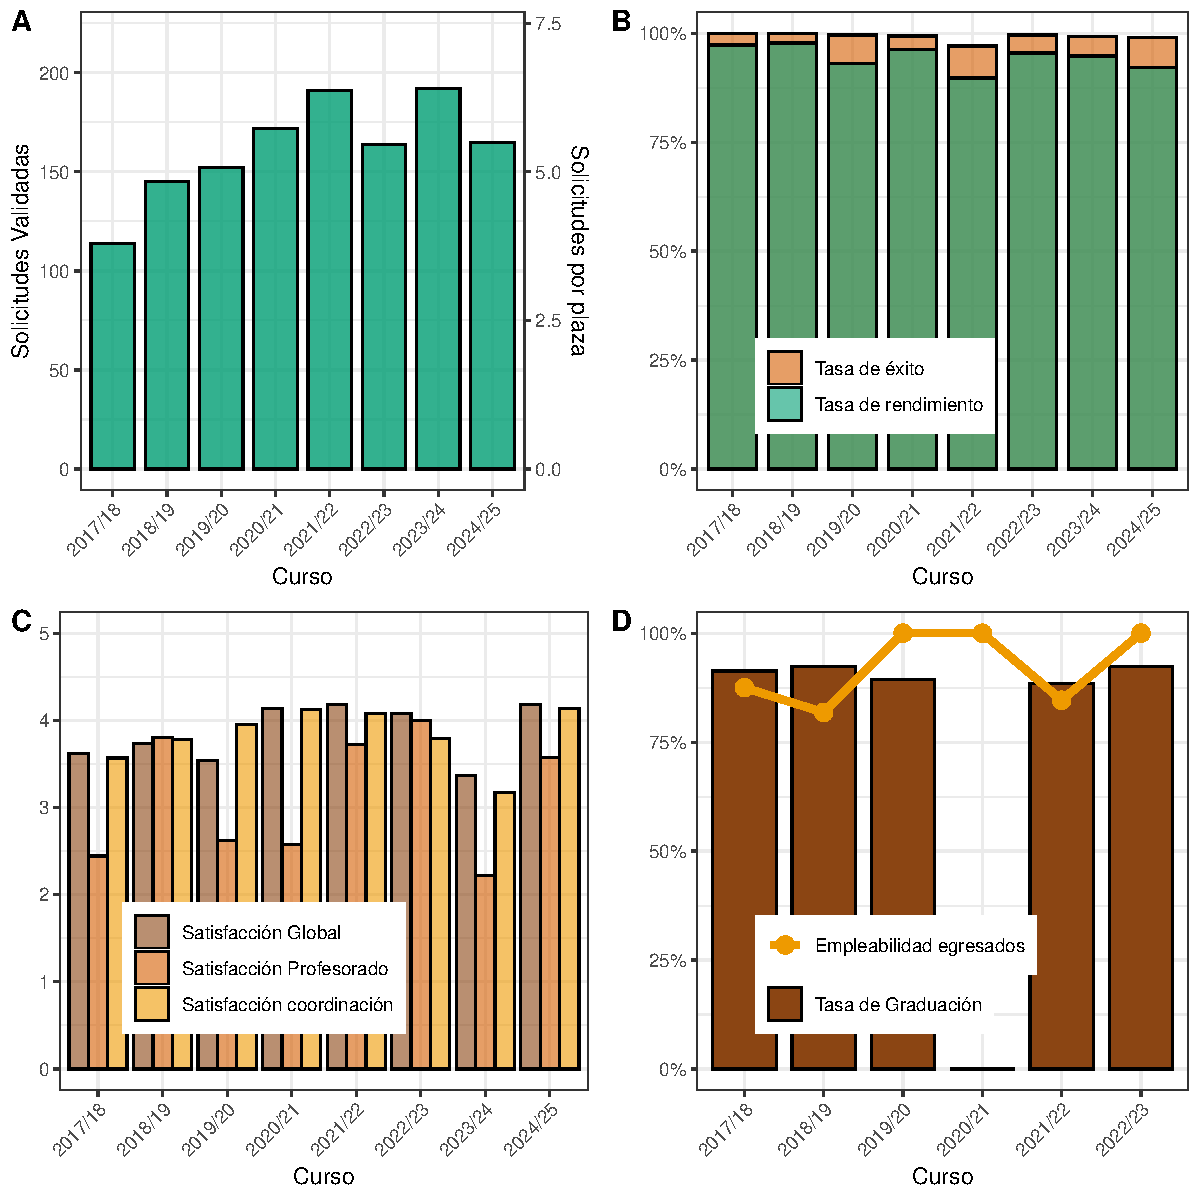
\includegraphics[keepaspectratio]{contexto_files/figure-pdf/fig-g3-1.pdf}}

}

\caption{\label{fig-g3}Evolución de la demanda (A), tasas de rendimiento
y éxito (B), satisfacción (C) y la empleabilidad de los egresados del
Máster en Bioinformática y Biología Computacional de la UAM. (D).
Fuente: UAMData.}

\end{figure}%

\clearpage

Como se muestra en la Figura~\ref{fig-g3}, se trata de un título con una
gran demanda, con un promedio de más de 5 solicitudes por cada una de
las 30 plazas ofertadas. Esto permite la selección de estudiantes con
formación y motivación altas, lo que redunda en una tasas de rendimiento
(créditos superados con el total de créditos matriculados) y éxito
(proporción de créditos superados sobre los créditos presentados)
superiores al 95\%. La satisfacción entre los estudiantes es alta, con
un claro descenso en los años de la pandemia de la COVID-19 y debido a
incidentes puntuales por falta de profesorado en una asignatura
(2022-23), que se están claramente recuperando en el último curso. Cabe
también destacar la alta empleabilidad del título, con casi el 90\% de
los egresados trabajando en el primer año según los datos de la UAM
hasta 2024.

Por último, como reflejo de la calidad de la enseñanza impartida y en el
contexto nacional caracterizado como se ha comentado por una oferta cada
vez más amplia de enseñanzas oficiales en bioinformática y biología
computacional en España, tanto en universidades públicas como privadas,
y particularmente intensificada en los últimos años por la incorporación
de nuevos títulos en el ámbito privado, el MUBBC ha sido recientemente
(noviembre 2025) como el primer Máster oficial de Bioinformática en
España que ha sido acreditado por la Sociedad Internacional de Biología
Computacional (ISCB).\footnote{\emph{Degree-Granting Endorsement
  Program} de la \emph{International Society for Computational Biology}
  (ISCB):
  \url{https://www.iscb.org/nucleus/education-and-training-resources/iscb-degree-granting-endorsement-program}
  \newline

  Más información:
  \url{https://www.uam.es/medicina/facultad/noticias/acreditacion-iscb-del-master-en-bioinformatica-y-bioogia-computacional-de-la-uam}}
Este programa de acreditación permite certificar aquellos programas que
cumplen con los estándares educativos de la ISCB en bioinformática y
biología computacional. La certificación garantiza a los futuros
estudiantes que el programa ha sido rigurosamente revisado y se ajusta a
los estándares profesionales, reforzando su credibilidad y prestigio
internacional. La solicitud para esta acreditación fue preparada por la
Coordinación del Máster, con la colaboración de varios profesores de la
Facultad y el asesoramiento de Enrique Carrillo, Profesor Asociado del
Máster entre los años 2017-2026 y en ese momento vocal de Docencia en la
Sociedad Española de Bioinformática y Biología Computacional (SEBiBC).

\subsection{Doctorado: El Programa de Doctorado en Biociencias
Moleculares.}\label{doctorado-el-programa-de-doctorado-en-biociencias-moleculares.}

El Departamento de Bioquímica es co-responsable del Programa de
Doctorado en Biociencias Moleculares y participa, asimismo, en el
Programa de Doctorado en Neurociencia, impartido por el Departamento de
Anatomía, Histología y Neurociencia en colaboración con el Instituto
Cajal del CSIC y otras instituciones académicas y de investigación
nacionales e internacionales.

El Programa de Doctorado en Biociencias Moleculares (PDBBMM) de la UAM,
regulado por el RD 99/2011, constituye una iniciativa conjunta del
Departamento de Biología Molecular de la Facultad de Ciencias y del
Departamento de Bioquímica de la Facultad de Medicina, con un
coordinador de cada Departamento. Los profesores del Departamento de
Bioquímica participan además como miembros de la Comisión Académica del
programa y como Tutores Académicos de las tesis. Al Tutor académico le
corresponde velar por la interacción de los doctorandos con la Comisión
Académica, revisando y validando la documentación enviada para la
evaluación anual de los doctorandos y colaborando en la mediación de los
posibles conflictos.

El objetivo fundamental del PDBBMM es la formación de investigadores
altamente cualificados, capaces de identificar y abordar problemas
científicos complejos en el ámbito de las Biociencias Moleculares,
liderar proyectos de investigación y contribuir de manera significativa
tanto a la generación de conocimiento como a su transferencia a la
sociedad, en particular en ámbitos relacionados con la biomedicina y la
biotecnología. En este contexto, el programa promueve la adquisición de
competencias avanzadas en el diseño, planificación y ejecución de
proyectos de investigación originales, así como en la aplicación del
método científico, el análisis crítico de datos y la interpretación
rigurosa de resultados (Feldon et al. 2011). La formación del doctorando
implica la integración de conocimientos especializados en áreas como la
biología molecular, la genética, la biomedicina y la biotecnología,
junto con el uso de metodologías experimentales y aproximaciones
computacionales, incluyendo el análisis de grandes volúmenes de datos,
la modelización de sistemas biológicos y la aplicación de herramientas
bioinformáticas (Attwood et al. 2019). Este enfoque permite al
doctorando desenvolverse en entornos científicos multidisciplinares y
altamente competitivos, facilitando su incorporación a equipos de
investigación de excelencia.

La actividad nuclear del programa se centra en la elaboración de la
tesis doctoral, concebida como un trabajo original de investigación que
debe constituir una aportación científica relevante y avanzar el estado
del conocimiento en su ámbito de especialización. Este proceso formativo
se complementa con un conjunto amplio de actividades que contribuyen al
desarrollo integral del investigador, incluyendo la asistencia a
seminarios y cursos especializados, la participación activa en congresos
nacionales e internacionales, la realización de estancias de
investigación en centros de prestigio y la elaboración de publicaciones
científicas en revistas especializadas. Estas actividades fomentan no
sólo la adquisición de conocimientos avanzados, sino también el
desarrollo de habilidades de comunicación científica, tanto oral como
escrita, en contextos internacionales.

El PDBBMM cuenta, además, con una sólida trayectoria y un reconocimiento
consolidado de su calidad, al derivar de programas de posgrado previos
que obtuvieron menciones de calidad y de excelencia a nivel nacional.
Además, el programa involucra investigadores de otras instituciones
colaboradoras de prestigio nacional e internacional: Centro de Biología
Molecular Severo Ochoa (CBMSO), Instituto de investigaciones Biomédicas
(IIB), Centro Nacional de Investigaciones Oncológicas (CNIO), Centro
Nacional de Investigaciones Cardiovasculares (CNIC), Centro Nacional de
Biotecnología (CNB), Centro de investigaciones Energéticas,
Medioambientales y Tecnológicas (CIEMAT), Instituto Cajal, Instituto de
Catálisis y Petroleoquímica (ICP), Centro Nacional de Microbiología del
ISCIII, Fundación Jiménez Díaz y los Hospitales Universitarios La Paz,
La Princesa, Puerta de Hierro y Gregorio Marañón.

En conclusión, el Programa de Doctorado en Biociencias Moleculares, es
de uno de los programas de mayor envergadura de la UAM, con una
contribución muy significativa a la formación doctoral y a la producción
científica de la universidad, consolidándose como un entorno formativo
de referencia en el ámbito de las biociencias.

\subsection{Docencia impartida por el candidato}\label{sec-yo}

Como complemento a la descripción precedente del entorno docente
inmediato de la plaza, resulta útil incorporar una síntesis visual de la
trayectoria docente desarrollada por el candidato en las distintas
titulaciones en las que ha participado entre los cursos 2018/2019 y
2025/2026, primero como Profesor Ayudante Doctor (desde septiembre 2018)
y luego como Profesor Permanente Laboral (desde noviembre 2023). La
Figura~\ref{fig-red} permite apreciar de forma conjunta la articulación
de esa actividad entre enseñanzas de grado y máster, así como las
relaciones estructurales y temáticas que conectan unas materias con
otras. En el caso del Grado en Bioquímica, la docencia se ha concentrado
de manera especialmente significativa en varias asignaturas obligatorias
del título, como \emph{Bioquímica Experimental Avanzada I},
\emph{Biosíntesis de Macromoléculas} y \emph{Bioinformática y Biología
Molecular de Sistemas}, junto con otras materias optativas del mismo
entorno, como \emph{Modelos Experimentales en Biomedicina Molecular} y
\emph{Herramientas de Programación en Bioquímica y Biología Molecular}.
Estas últimas, y en particular la docencia en programación aplicada,
ponen de manifiesto una línea de trabajo que enlaza de forma natural con
la formación especializada del Máster en Bioinformática y Biología
Computacional. En este contexto, \emph{Bioinformática Estructural} ocupa
una posición particularmente relevante, no solo por su papel dentro de
la docencia del máster, sino también por situarse en la intersección
entre bioquímica estructural, modelización y bioinformática, lo que la
convierte en un marco especialmente adecuado para la propuesta
metodológica que se desarrollará en el capítulo siguiente.

Por otra parte, tanto el bloque de replicación y reparación del DNA
impartido en \emph{Biosíntesis de Macromoléculas} como la clase
impartida anualmente en asignatura de posgrado \emph{Replicación,
Reparación e Inestabilidad de Genomas,} así como el bloque de contenidos
que incluye replicación y amplificación del DNA e introducción a las
tecnologías ómicas del complemento de bioquímica y biología molecular
del MUBBC, guardan una relación especialmente estrecha con la línea de
investigación desarrollada por el candidato a lo largo de su trayectoria
académica, reforzando así la conexión entre actividad investigadora y
actividad docente.

Considerada en su conjunto, esta trayectoria no solo refleja una
docencia sostenida y diversa en asignaturas de grado y posgrado, sino
también una implicación continuada en el propio desarrollo del Máster en
Bioinformática y Biología Computacional, cuya coordinación fue asumida
por el candidato entre junio de 2021 y junio de 2026.

\begin{figure}[H]

\centering{

\pandocbounded{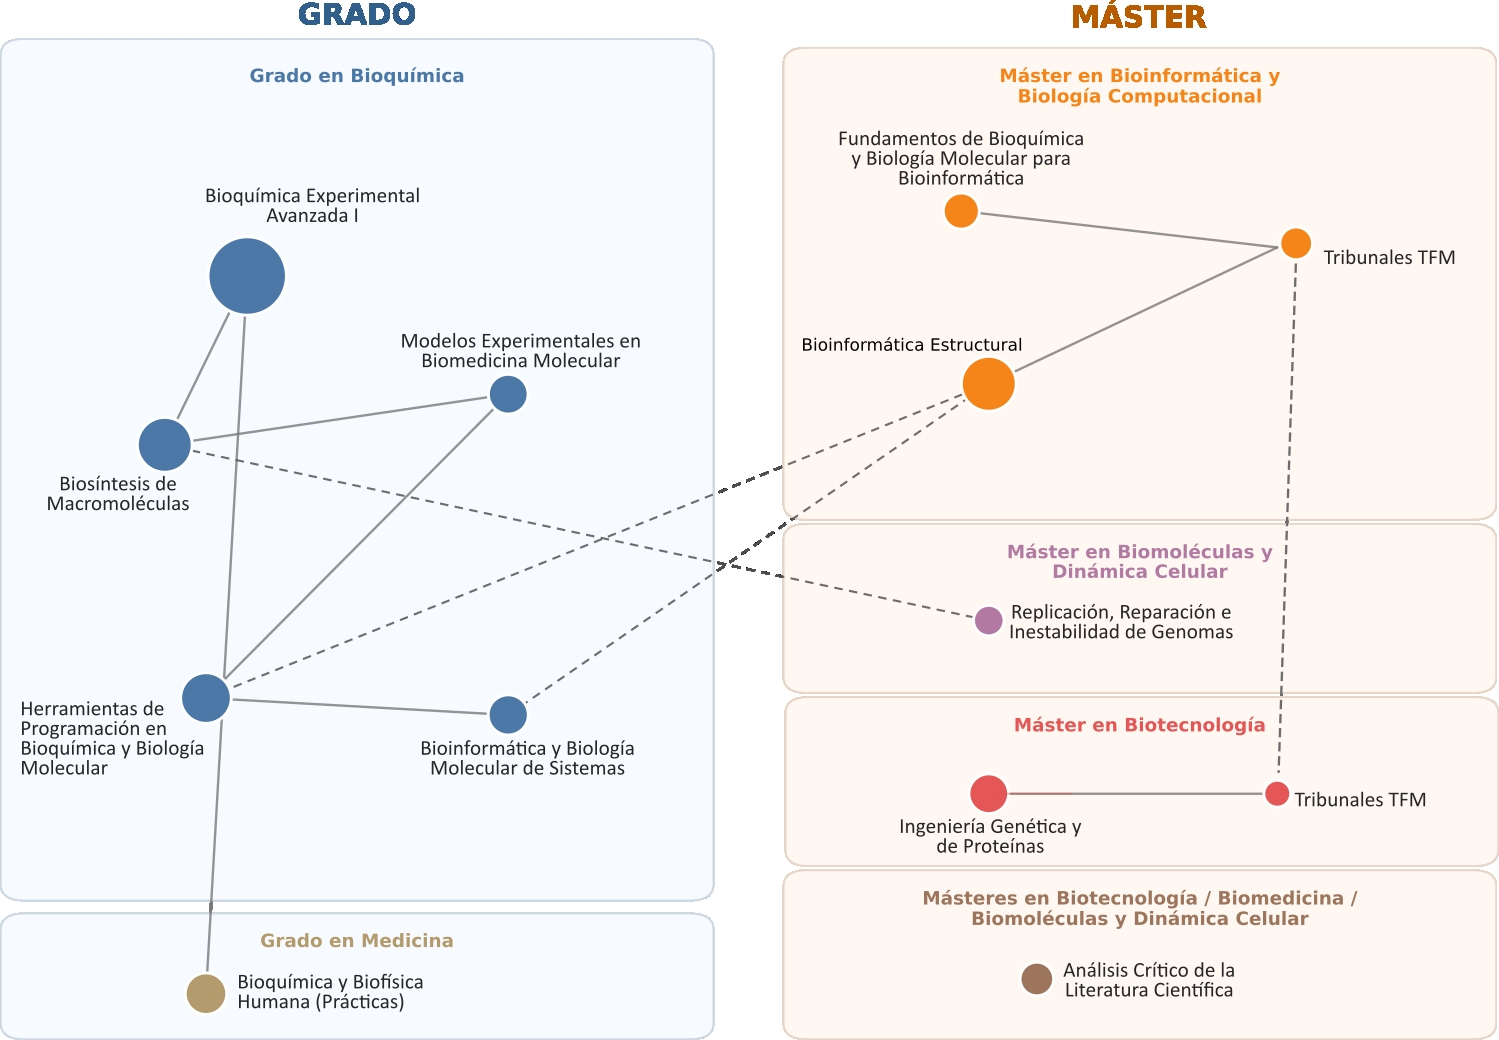
\includegraphics[keepaspectratio]{images/red.jpg}}

}

\caption{\label{fig-red}Docencia impartida por el candidato. Cada nodo
representa una asignatura su tamaño es proporcional al total de horas
impartidas acumuladas en el periodo considerado. Las aristas continuas
enlazan materias pertenecientes a un mismo título o relacionadas
estructuralmente dentro de una misma titulación, mientras que las
aristas discontinuas indican relaciones temáticas entre asignaturas de
distintos contextos docentes.}

\end{figure}%

\bookmarksetup{startatroot}

\chapter{Propuesta de mejora en el uso de metodologías de aprendizaje
activo en bioinformática}\label{sec-pro}

Este capítulo se articula en dos partes complementarias. En primer
lugar, la Sección~\ref{sec-ens} presenta un marco de reflexión general
sobre los principales modelos de enseñanza en educación superior, con
especial atención a las metodologías de aprendizaje activo, la
evaluación del aprendizaje y el impacto reciente de la inteligencia
artificial generativa en la docencia universitaria. Esta revisión no
constituye un excurso teórico independiente, sino el fundamento
conceptual necesario para situar y justificar la propuesta docente que
se desarrolla después. En segundo lugar, la Sección~\ref{sec-42}
traslada este marco general a un contexto académico concreto, mediante
una propuesta de mejora aplicada a la asignatura Bioinformática
Estructural del Máster en Bioinformática y Biología Computacional de la
UAM. De este modo, el capítulo avanza desde la reflexión pedagógica
general hacia su concreción en una experiencia docente específica,
permitiendo mostrar la coherencia entre principios metodológicos, diseño
de actividades, evaluación y mejora continua del aprendizaje.

\section{Modelos de enseñanza en la educación superior}\label{sec-ens}

Los objetivos docentes expresan los rasgos y capacidades generales de
los profesionales que queremos formar en nuestros estudiantes y expresan
resultados previstos de aprendizaje. Las orientaciones para la
construcción del EEES, sugieren que se formulen objetivos como logros de
aprendizaje en términos de competencias. De esta forma, los planes de
estudios implementados actualmente en la Universidad están basados en un
sistema de enseñanza que consiste en que el estudiante vaya adquiriendo
gradualmente competencias concretas por lo que se orientan,
fundamentalmente, a los resultados de aprendizaje. Las competencias
educativas son la combinación integrada de conocimientos, habilidades y
actitudes que se ponen en acción para un desempeño adecuado en un
contexto dado. Según el proyecto Tuning Educational Structures in Europe
(Sánchez 2008), conocido como Proyecto Tuning, las competencias pueden
definirse de esta forma:

\begin{quote}
``Las competencias representan una combinación dinámica de atributos, en
relación con conocimientos, habilidades, actitudes y responsabilidades,
que describen los resultados del aprendizaje de un programa educativo o
el que los estudiantes son capaces de demostrar al final de un proceso
formativo.''
\end{quote}

Su uso debe posibilitar un marco común de cualificación que permita el
reconocimiento de los Títulos. Con las competencias se integran los tres
pilares fundamentales que debe desarrollar la educación superior:
``saber'', conocimientos teóricos de un campo académico; ``saber
hacer'', habilidades, aplicaciones prácticas y operativas del
conocimiento y ``saber estar'', valores como parte integrante de la
forma de percibir a los otros y vivir en un contexto social. El proyecto
Tuning considera que las competencias específicas, aquellas relacionadas
con los conocimientos, son lo que debe ``saber'' el alumno al terminar
el programa mientras que las competencias genéricas o transversales, son
comunes a casi todas las profesiones y titulaciones universitarias y se
refieren a lo que el alumno debe ``saber hacer'' al terminar el proceso
de aprendizaje.

\subsection{La lección magistral o
expositiva}\label{la-lecciuxf3n-magistral-o-expositiva}

La lección expositiva es quizás uno de los recursos más utilizados por
los docentes y está comprobado que este tipo de técnica es muy útil en
la formación universitaria y consiste en la exposición detallada de los
contenidos de un tema de forma oral. Habitualmente la lección magistral
se apoya en medios audiovisuales para mejorar la comprensión o reforzar
el mensaje. Se trata de un método que facilita la transmisión de
información, especialmente en grupos grandes de alumnos. Sin embargo, en
los últimos años su uso se ha cuestionado puesto que puede fomentar la
pasividad o el aburrimiento, dificulta la atención sostenida y no
siempre evalúa si el alumno ha comprendido o asimilado la información.
De hecho, se considera como una de las causas del absentismo de los
estudiantes. Especialmente en la sociedad actual, en la que el
conocimiento está al alcance de un \emph{clic}, es necesario que la
asistencia a clase les aporte algo más que una colección de
conocimientos. El EEES reconoce la necesidad de que el alumnado no solo
adquiera conocimientos, sino que desarrolle competencias transversales
como la resolución de problemas, el pensamiento crítico, la autonomía,
la colaboración y la capacidad de aplicar lo aprendido a situaciones
nuevas (Fernández Fernández and Madinabeitia Ezkurra 2020).

Existe por tanto una necesidad de evolución de la actividad de los
docentes en el aula, ya que al profesor universitario se le va a pedir
que pueda ser capaz de realizar actividades y promover ambientes de
trabajo que estén basados en la reflexión y en el diálogo. En este
sentido existe toda una variedad de métodos docentes que buscan
favorecer la comprensión integral del tema, por encima de la acumulación
de conocimientos. Por ejemplo, la denominada \textbf{Lección Magistral
Interactiva} (Iglesias-Soilán et al. 2024; Morell Moll 2004) busca
estimular la comprensión y la aplicación de los conceptos mediante la
interacción entre el docente y los estudiantes, y entre los propios
estudiantes. Esta lección magistral interactiva comparte los tres mismos
puntos que su análoga tradicional: una introducción, en la que se
presenta un concepto; el desarrollo del contenido y una finalización o
resumen. Entonces, ¿cuáles son las diferencias entre ambas versiones? En
la introducción de la interactiva, se plantea un contexto real de ese
concepto y no aislado de su entorno, al tiempo que deja a un lado la
unidireccionalidad en su desarrollo, buscando constantemente las
preguntas, dudas, reflexiones, objeciones\ldots{} para, en su
finalización o resumen, acoger las opiniones de todas las partes (Morell
Moll 2004). Para esto, pueden utilizarse técnicas y herramientas como el
método socrático moderno, el debate y los \emph{roleplayings}, apostando
por la continua interacción del profesor con sus estudiantes.

En conclusión, la lección magistral tradicional está evolucionando hacia
un modelo más interactivo, progresivamente más centrado en el alumnado.
Al introducir elementos de participación, diálogo y aplicación de los
conceptos durante la propia exposición, este enfoque aproxima la lección
magistral a los principios del aprendizaje activo, aunque sin abandonar
completamente su estructura tradicional. Esta evolución pone de
manifiesto un cambio más amplio en la concepción de la enseñanza
universitaria, que se concreta en el desarrollo de metodologías de
aprendizaje activo.

\subsection{Metodologías de aprendizaje
activo}\label{metodologuxedas-de-aprendizaje-activo}

Bajo el término general de aprendizaje activo se agrupa un conjunto
amplio de estrategias docentes que comparten una idea central: el
aprendizaje mejora cuando el estudiante participa cognitivamente en la
tarea, toma decisiones, contrasta ideas, aplica conceptos, resuelve
problemas, argumenta, explica o colabora con otros. Esta concepción no
se identifica con una técnica única ni con un formato cerrado, sino que
puede concretarse en metodologías diversas, como el aprendizaje basado
en problemas o proyectos, el aula invertida, el aprendizaje cooperativo,
la gamificación, el \emph{learning by doing} o el análisis de casos. En
todas ellas, el elemento común no es necesariamente la herramienta
empleada, sino el tipo de actividad intelectual que se promueve en el
alumnado. La base del aprendizaje activo es el \textbf{constructivismo},
corriente pedagógica que defiende la enseñanza basada en el alumnado y
en la forma en la que se aprenden conceptos complejos, relacionando el
conocimiento previo con los nuevos conocimientos, siendo ellos los
actores principales de su propio aprendizaje (Ramsden 2003). En este
contexto, el aprendizaje cooperativo ha sido descrito como una de las
bases sobre las que se construyen muchas estrategias de éxito en el
aprendizaje activo, al estructurar la interdependencia positiva, la
responsabilidad individual y la interacción promotora entre estudiantes
(Johnson and Johnson 2018).

La evidencia acumulada en disciplinas \emph{STEM} (acrónimo en inglés de
\emph{Science, Technology, Engineering, and Mathematics}: Ciencia,
Tecnología, Ingeniería y Matemáticas) respalda la utilidad de estas
aproximaciones, mostrando un incremento del rendimiento en exámenes y
contribuyendo además a reducir las brechas de género o grupo social en
el rendimiento en estas asignaturas, especialmente cuando se aplican con
suficiente intensidad y se combinan con prácticas docentes inclusivas
(Theobald et al. 2020).

Sin embargo, la implantación de estas metodologías en la universidad no
está exenta de limitaciones y dificultades. En primer lugar, la
resistencia a modificar la tradicional lección magistral se relaciona
con factores institucionales y culturales, como la presión por cubrir
temarios extensos, la escasez de tiempo y recursos del profesorado, la
sobrecarga docente o la falta de formación pedagógica específica. Así
por ejemplo, algunos autores han descrito la ``tiranía de la cobertura
de contenidos'' como una barrera importante para adoptar enfoques
centrados en el aprendizaje, ya que el deseo de transmitir todo el
programa puede desplazar actividades que favorecen una comprensión más
profunda y transferible. Además, se puede generar la ilusión de que el
aprendizaje activo es la ``bala mágica'' que siempre va a funcionar por
definición (Gooblar (2019)), lo que puede llevar a la frustración y
desencanto si los primeros intentos no cumplen con las expectativas.
Asimismo, diversos estudios sobre profesorado universitario señalan que
las concepciones docentes centradas en la transmisión de contenidos y la
identidad profesional más vinculada a la investigación que a la docencia
pueden dificultar la transición hacia modelos más activos (Petersen et
al. 2020; Pineda-Alfonso and Duarte Piña 2020). En conclusión, el diseño
de cursos basados en aprendizaje activo puede suponer una tarea costosa,
que además de a la dificulad intrínsica del diseño docente, se enfrenta
a retos como son el cambio de métodos y rutinas largamente establecidas
y la sobrecarga de alumnos y profesores, por lo que suele ser
recomendable una introducción progresiva.

Es importante también aclarar que el aprendizaje activo no equivale
necesariamente al uso de tecnologías de la información y la
comunicación. Las tecnologías de información y comunicación (TIC) pueden
facilitar determinadas formas de participación, evaluación formativa,
análisis de datos, comunicación o trabajo colaborativo, pero no
constituyen por sí mismas una metodología activa. Una clase puede
incorporar plataformas virtuales, cuestionarios en línea, repositorios
digitales o entornos computacionales y seguir respondiendo a un modelo
esencialmente transmisivo si el estudiante permanece en una posición
pasiva. Del mismo modo, es posible desarrollar aprendizaje activo sin
tecnología digital, mediante discusión guiada, resolución de problemas
en grupo, análisis de casos, debates estructurados o dinámicas
cooperativas. Esta distinción es coherente con la idea de que el efecto
educativo de la tecnología depende en gran medida del diseño pedagógico
en el que se integra, más que de la mera presencia del recurso
tecnológico (Valverde-Berrocoso et al. 2022).

Entre las disciplinas que se pueden encuadrar como STEM, la
bioinformática es una disciplina situada en la intersección entre la
biología, la informática, la estadística y el análisis de datos.
Aprender bioinformática no consiste únicamente en memorizar
procedimientos para usar herramientas de análisis o recordar algoritmos,
formatos de archivo o bases de datos, sino en desarrollar la capacidad
de formular preguntas biológicas, seleccionar herramientas adecuadas,
interpretar resultados, detectar limitaciones metodológicas y reproducir
análisis de forma rigurosa. Por ello, la enseñanza de la bioinformática
se beneficia de metodologías que aproximen al alumnado a problemas
reales o verosímiles: análisis de secuencias, anotación funcional,
comparación de genomas, estudio de expresión génica, filogenia,
metagenómica, modelado estructural o integración de datos ómicos. El
aprendizaje basado en proyectos ofrece un marco especialmente adecuado
para este tipo de docencia, porque permite aprender aplicando ideas a
situaciones auténticas y próximas a la práctica científica real (Krajcik
and Blumenfeld 2005). En esta línea hay bastantes estudios publicados
que muestran, por ejemplo, como la enseñanza de programación mediante
seminarios basados en proyectos y elementos de aula invertida, guiando
al alumnado a través de flujos de trabajo propios de la ciencia de
datos, incluyendo gestión, transformación, visualización y comunicación
de resultados, mejoran el aprendizaje profundo (Meyer 2021).

\subsection{Evaluación del aprendizaje en el contexto del
EEES}\label{evaluaciuxf3n-del-aprendizaje-en-el-contexto-del-eees}

La evaluación del aprendizaje es un componente esencial del proceso de
enseñanza-aprendizaje y debe entenderse como un proceso continuo y
coherente con los objetivos formativos y las metodologías empleadas. En
el contexto del Espacio Europeo de Educación Superior, su función no se
limita a comprobar los conocimientos adquiridos, sino que debe
contribuir también al desarrollo de competencias y a la mejora del
propio proceso educativo.

Es importante además distinguir entre evaluación y calificación. La
evaluación implica recoger, analizar e interpretar información sobre el
aprendizaje del estudiante con el fin de orientar su mejora. La
calificación, en cambio, es la expresión final de los resultados
obtenidos, normalmente en forma numérica o cualitativa. Mientras que la
calificación cumple sobre todo una función acreditativa y
administrativa, la evaluación tiene un alcance más amplio y una función
formativa, reguladora y orientadora del aprendizaje (López Pastor 2009).

Desde esta perspectiva, la evaluación debe integrarse de manera natural
en el proceso educativo, superando enfoques basados exclusivamente en
pruebas finales y favoreciendo un seguimiento continuo del progreso del
estudiante. En este sentido, cobra especial importancia la evaluación
formativa, entendida como aquella que ayuda a desarrollar competencias
de aprendizaje permanente y de autorregulación. Este enfoque se alinea
con una enseñanza activa, centrada en el estudiante y orientada al
desarrollo de competencias. Además, favorece que el alumnado tome
conciencia de qué aprende, cómo lo aprende y qué estrategias puede
desarrollar para seguir avanzando (López Pastor 2009).

No obstante, para que la evaluación tenga un carácter verdaderamente
formador no basta con incorporar técnicas como la autoevaluación o la
coevaluación. Es necesario que el estudiante participe activamente en el
análisis de sus errores, en la identificación de sus dificultades y en
la elaboración de estrategias para superarlas. En este sentido, adquiere
especial relevancia la idea de evaluación formadora, que pone el énfasis
en el valor educativo de las propias actividades de evaluación. La
evaluación formativa deja así de ser un mero instrumento para comunicar
resultados y se convierte en una oportunidad de aprendizaje en sí misma.

El cambio de paradigma impulsado por el EEES ha supuesto también una
transición desde modelos centrados en el profesor hacia modelos
centrados en el aprendizaje del estudiante. En este contexto, resulta
más apropiado hablar de actividades de enseñanza-aprendizaje que de
métodos docentes, ya que lo relevante es la interacción entre ambos
procesos. La evaluación debe, por tanto, alinearse con esas actividades
y centrarse no solo en los resultados obtenidos, sino también en los
procesos seguidos para alcanzarlos.

El sistema de evaluación influye de forma decisiva en el tipo de
aprendizaje que desarrollan los estudiantes. Un modelo basado casi
exclusivamente en exámenes finales tiende a favorecer formas de estudio
más superficiales, centradas en la memorización y la reproducción de
contenidos. Por el contrario, una evaluación continua, diversificada y
orientada a la reflexión favorece una comprensión más profunda, la
integración de conocimientos y la capacidad de transferirlos a nuevos
contextos. Del mismo modo, la incorporación de enfoques dialógicos,
basados en la interacción, el debate y la construcción compartida del
conocimiento, contribuye al desarrollo de competencias complejas propias
de la formación universitaria.

De acuerdo con estos principios, la evaluación del aprendizaje debe
basarse en criterios de validez, fiabilidad, objetividad y
transparencia, garantizando su adecuación a los resultados de
aprendizaje y a las competencias establecidas. Resulta igualmente
esencial que el alumnado conozca con claridad los criterios y
procedimientos de evaluación, favoreciendo así su implicación activa en
el proceso. La retroalimentación constituye otro elemento clave, al
proporcionar información útil tanto al estudiante como al docente para
la mejora continua de los procesos de enseñanza-aprendizaje.

Finalmente, la evaluación debe concebirse como un proceso dinámico y
abierto, susceptible de revisión y mejora a partir del análisis de los
resultados obtenidos y de la experiencia acumulada. En este sentido, no
solo cumple una función de acreditación del aprendizaje, sino que
también actúa como una herramienta importante para la innovación docente
y el perfeccionamiento progresivo de la práctica educativa. Proporcionar
comentarios de retroalimentación o \emph{feedback} durante el proceso de
aprendizaje, y no solo al final, resulta especialmente valioso. En
muchos casos, incluir una calificación en ese \emph{feedback} es
innecesario e incluso contraproducente, mientras que puede ser más útil
centrar la atención en la mejora del aprendizaje en etapas intermedias
(Ruiz Martín 2020).

En este contexto, resulta especialmente relevante el diseño y uso de
herramientas que permitan una evaluación más transparente, objetiva y
coherente con los resultados de aprendizaje, como las rúbricas, las
listas de control o los mapas de objetivos. Estos instrumentos ayudan a
explicitar los criterios de evaluación y pueden mejorar tanto la
coherencia de la corrección como la calidad de la retroalimentación. No
obstante, su elaboración requiere tiempo y una reflexión cuidadosa sobre
qué evidencias de aprendizaje son realmente relevantes, y su uso
excesivamente rígido puede limitar la creatividad o simplificar en
exceso la complejidad de ciertos trabajos (Cano 2015). Al mismo tiempo,
la generalización de la evaluación continua y la necesidad de ofrecer
\emph{feedback} frecuente y útil plantean una dificultad práctica
evidente en muchos contextos universitarios debido a la carga de trabajo
de docentes y alumnos. En este escenario han empezado a adquirir
protagonismo nuevas herramientas digitales interactivas capaces de
apoyar determinados procesos de revisión, comentario y seguimiento del
aprendizaje. Entre ellas, la inteligencia artificial generativa (IAG)
ocupa una posición especialmente visible, lo que obliga a examinar
críticamente sus posibilidades y sus límites en el ámbito de la docencia
universitaria.

\subsection{La inteligencia artificial generativa en la docencia
universitaria}\label{sec-ia}

A pesar de que su uso se ha generalizado recientemente, la irrupción de
la inteligencia artificial generativa (IAG) constituye un cambio de
alcance amplio que afecta también a la universidad. Su rápida expansión
obliga a revisar cómo se enseña, cómo se aprende y cómo se evalúa,
especialmente en cuestiones relacionadas con la autenticidad del
aprendizaje, la autoría académica y la garantía de los resultados
formativos. Esta reflexión es especialmente urgente si se tiene en
cuenta que el alumnado universitario español se sitúa entre los que más
utilizan estas herramientas a nivel internacional
(Figura~\ref{fig-iag}). En esta línea, un informe reciente (CYD 2026)
señala que un 86\% de los estudiantes en universidades españolas usa
herramientas de IAG, lo que ha cambiado su forma de estudiar para un
66\% de ellos, llevando a un 27\% a asistir menos a clase.

En este contexto, el informe de la Conferencia de Rectores de las
Universidades Españolas (CRUE) sobre la IAG en la docencia universitaria
señala que la cuestión ya no es si la universidad debe relacionarse con
estas herramientas, sino cómo, cuándo y para qué debe hacerlo,
integrándolas con criterios pedagógicos explícitos, transparentes y
alineados con los objetivos formativos (Cruz Argudo et al. 2024). En la
misma línea, la \emph{Guía Básica para el uso de IA por profesores y
estudiantes}, publicada por la UAM en 2023\footnote{Disponible en
  \url{https://www.uam.es/uam/media/doc/1606941290988/guia-visual-iagen.pdf}},
insiste en la necesidad de delimitar con claridad el uso de estas
herramientas y su relación con la evaluación. De hecho, las guías
docentes de la UAM para el curso 2026-27 establecen expresamente que el
uso de tecnologías de IAG no debe sustituir la participación activa del
estudiantado en la realización de tareas evaluables ni la adquisición
real de los resultados de aprendizaje previstos.

\begin{figure}

\centering{

\pandocbounded{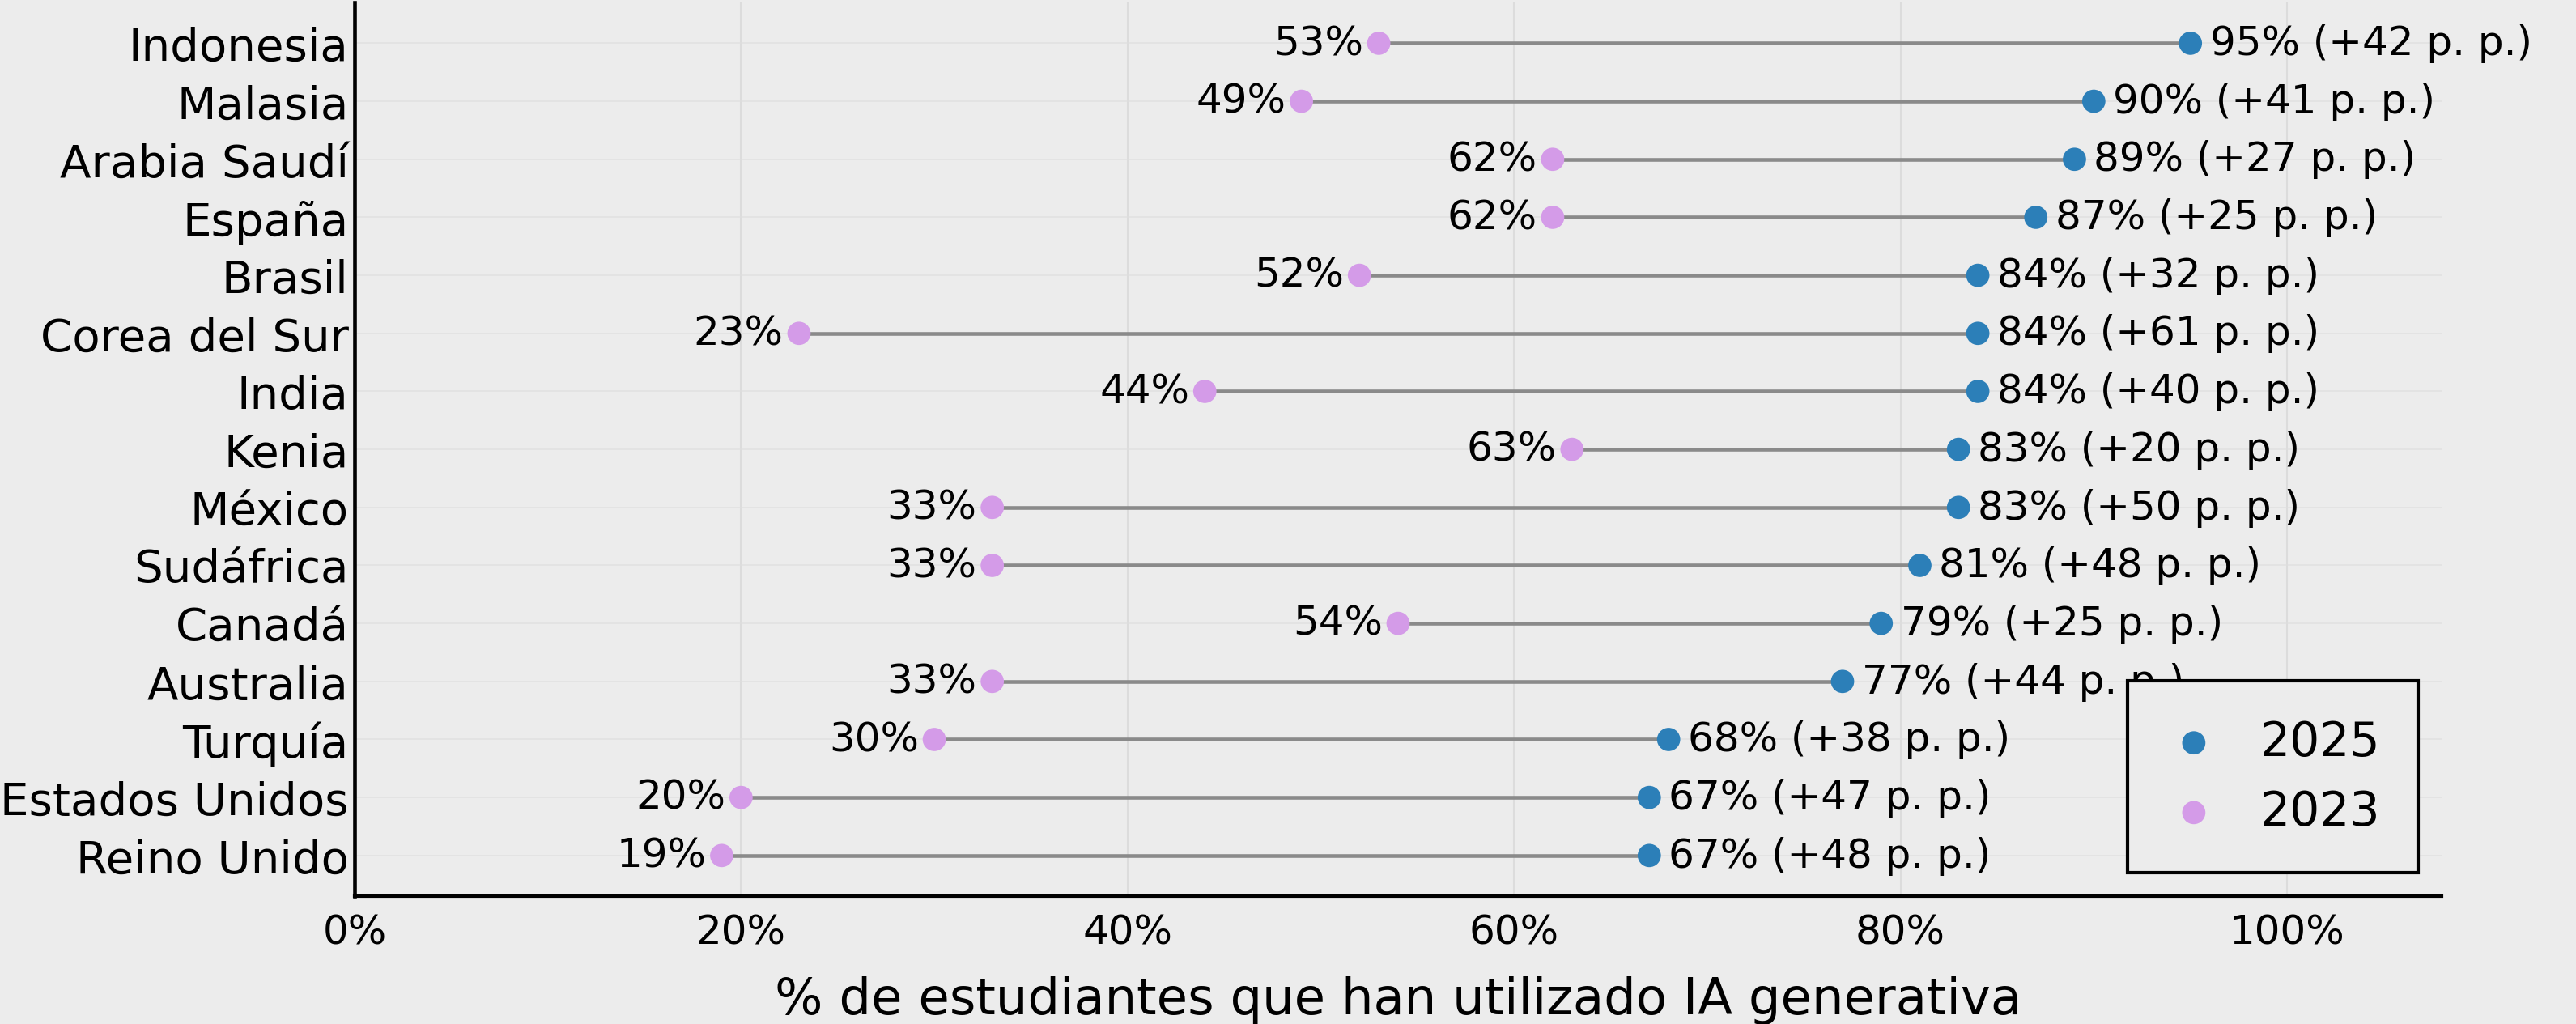
\includegraphics[keepaspectratio]{images/figura_IAG_estudiantes.png}}

}

\caption{\label{fig-iag}Estudiantes universitarios (\%) por país que han
usado inteligencia artificial generativa en sus estudios. Modificado de
Sajadieh et al. (2026).}

\end{figure}%

La incorporación de la IAG en la universidad es ya una realidad que
proporciona grandes oportunidades para mejorar la formación de todos
nuestros estudiantes, si bien supone también un desafío (Liu et al.
2023), lo que exige definir con claridad sus usos, límites y
condiciones. Las orientaciones institucionales advierten de riesgos
importantes: generación de información inexacta o sesgada, opacidad de
los sistemas, problemas de privacidad y protección de datos, y amenazas
a la integridad académica cuando el trabajo intelectual del estudiante
se sustituye por respuestas automatizadas. A ello se añade el riesgo de
\emph{delegación cognitiva}, entendido como la transferencia a la IAG de
tareas de análisis, decisión o creación que deberían formar parte del
propio proceso de aprendizaje. Si esta delegación reduce el esfuerzo
intelectual del estudiante, puede debilitar precisamente las capacidades
que la universidad debe fomentar: comprensión, razonamiento crítico,
autonomía y autoría académica. Por ello, la integración de estas
herramientas requiere un enfoque centrado en la persona y una evaluación
ética y pedagógica rigurosa (Miao and Holmes 2024). En la misma
dirección, las orientaciones europeas subrayan la necesidad de reforzar
una alfabetización crítica de profesores y alumnos que permita tomar
decisiones informadas, responsables y adecuadas a cada contexto
(Directorate-General for Education 2026). La respuesta universitaria no
debería limitarse, por tanto, al control del uso de la IAG, sino
orientar la docencia y la evaluación hacia aprendizajes significativos,
pensamiento crítico, presencialidad activa, autoría académica y uso
responsable de la tecnología.

Bien integrada, la IAG puede contribuir al desarrollo de competencias
relevantes en la educación superior, como el pensamiento crítico, la
formulación de preguntas, la verificación de fuentes, la comunicación,
la creatividad, la resolución de problemas y la revisión del propio
trabajo. Entendida así, la IA no actúa como un atajo que sustituye el
aprendizaje, sino como una herramienta que puede apoyar el desarrollo de
competencias académicas y profesionales de alto valor, cada vez más
demandadas en el entorno laboral (Organisation for Economic Co-operation
and Development 2024).

Adaptar la docencia y la evaluación al entorno de la inteligencia
artificial no es solo una cuestión técnica o normativa; implica también
decidir qué tipo de aprendizaje quiere promover la universidad. En este
sentido, la integración de metodologías de aprendizaje activo con usos
formativos de la IAG se alinea con las prioridades estratégicas de la
UAM en el marco del proceso participativo \emph{UAM Futuro 2026-2030},
disponible en el portal de participación de la universidad
(\url{https://participa.uam.es/}).

Esta orientación hacia usos formativos concretos empieza a reflejarse en
experiencias recientes en áreas próximas a la biología molecular, la
bioquímica y, de forma especialmente clara, la bioinformática. En estos
contextos, la IAG no se plantea solo como una herramienta de redacción,
sino como apoyo para adquirir competencias complejas, manteniendo la
prioridad conceptual y el criterio científico subyacentes (Teufel and
Liberles 2026). En bioinformática para principiantes, por ejemplo, se ha
propuesto un modelo iterativo de trabajo con ChatGPT basado en la mejora
progresiva de \emph{prompts}, la identificación de errores y la
validación de resultados. El objetivo no es obtener una respuesta
automática, sino aprender a formular bien el problema, interpretar la
solución propuesta y comprobar críticamente su validez en tareas de
análisis de datos bioinformáticos (Shue et al. 2023).

Otros trabajos apuntan en la misma dirección en la intersección entre
biología molecular y análisis computacional. Un estudio reciente mostró
que estudiantes de biología sin experiencia previa en programación
podían utilizar ChatGPT para generar código en Python y analizar
conjuntos de datos reales de secuenciación masiva (NGS), guiando la
interacción con la herramienta desde su propio conocimiento biológico
(Delcher et al. 2025). Este tipo de experiencias resulta especialmente
relevante porque muestra que la IAG puede actuar como andamiaje para
reducir la barrera de entrada a la programación y al análisis ómico. De
este modo, estudiantes con perfiles más experimentales pueden
aproximarse de forma activa a tareas computacionales que antes les
resultaban menos accesibles (Wang et al. 2024). En conjunto, la
integración de la IAG en la enseñanza de biociencias aumenta la
motivación, el aprendizaje y la inclusividad de los estudiantes y,
adicionalmente, produce un impacto en su futura vida laboral, que
requerirá el uso de IAG de manera habitual (Cotton and Cotton (2026)).

Ahora bien, este potencial solo se mantiene si la herramienta se integra
en un diseño docente exigente. La IAG debe utilizarse de forma
complementaria a otras estrategias, como el contraste de resultados y la
participación real del estudiante en la toma de decisiones. Su uso
generalizado y poco reflexivo puede generar dependencia, homogeneizar
las respuestas y crear una falsa sensación de competencia (Torres et al.
2023; Jácome Ayala and Checa Cabrera 2025). Por ello, conviene orientar
su uso hacia pasos concretos del aprendizaje, tales como traducir una
pregunta biológica a una estrategia analítica, discutir parámetros,
detectar errores en el código, comparar soluciones alternativas y
justificar la interpretación final de los resultados. Algunos estudios
muestran, además, que aunque los estudiantes reconocen la utilidad de la
IAG para aprender programación, buscar soluciones o diseñar algoritmos,
con frecuencia siguen prefiriendo sus propias soluciones frente a las
generadas por estas herramientas (Frydenberg et al. 2025).

En conjunto, las experiencias publicadas apuntan a una conclusión clara:
bien diseñada, la IAG puede ampliar el acceso a competencias de
programación, análisis de datos y resolución de problemas en ciencias de
la vida; mal orientada, puede fomentar dependencia, reducir la autoría
intelectual y debilitar la validación crítica de los resultados (Suresh
et al. 2025; Wang et al. 2024; Jácome Ayala and Checa Cabrera 2025).

\section{Propuesta de aprendizaje activo en la asignatura Bioinformática
Estructural}\label{sec-42}

A partir del marco pedagógico desarrollado en la Sección~\ref{sec-ens},
la presente sección presenta una propuesta docente aplicada a la
asignatura Bioinformática Estructural del Máster en Bioinformática y
Biología Computacional. Esta asignatura constituye un contexto
especialmente adecuado para trasladar al plano práctico los principios
analizados previamente, ya que en ella convergen la necesidad de
promover un aprendizaje activo basado en proyectos, el uso de
estrategias de evaluación formativa y la posibilidad de incorporar
herramientas de inteligencia artificial generativa como apoyo al
feedback y a la mejora autónoma del trabajo académico, en línea con lo
expuesto previamente (Sección~\ref{sec-ia}). De este modo, la propuesta
que se desarrolla a continuación pretende mostrar cómo estos elementos
pueden articularse de manera coherente en una experiencia docente
concreta, orientada a reforzar tanto la adquisición de competencias
específicas como el desarrollo de habilidades transversales

\subsection{Descripción de la asignatura en contexto del Máster en
Bioinformática y Biología
Computacional}\label{descripciuxf3n-de-la-asignatura-en-contexto-del-muxe1ster-en-bioinformuxe1tica-y-biologuxeda-computacional}

La asignatura \textbf{Bioinformática Estructural} (código asignatura UAM
33082) es una asignatura obligatoria de 3 ECTS que se imparte en el
Máster de Bioinformática desde su implantación en el curso 2017-18
(Sección~\ref{sec-MUBBC}). Originalmente se impartía en el primer
cuatrimestre, pero con la reestructuración del plan de estudios, a
partir del curso 2024-25 se imparte en el segundo. Este cambio, junto
con los ajustes introducidos en contenidos y resultados de aprendizaje,
focalizando más la asignatura en modelado molecular y sus aplicaciones e
incluyendo un bloque de acoplamiento (\emph{docking}) de ligandos. El
cambio de cuatrimestre ha permitido también mejorar diversos aspectos
metodológicos del trabajo práctico, ya que los estudiantes cuentan a
estas alturas con una mayor formación en programación, tanto en Python
como en R, lo que facilita el desarrollo de pequeños \emph{pipelines}
para el análisis computacional de estructuras.

Dentro del plan de estudios del Máster, la asignatura actúa como un
puente entre la información biológica derivada de las secuencias y la
comprensión mecanística de los sistemas biológicos a nivel molecular.
Mientras que otras materias se centran principalmente en el análisis de
genomas, transcriptomas, redes biológicas o modelos predictivos,
Bioinformática Estructural introduce al estudiantado en el estudio de la
relación entre secuencia, estructura y función de biomoléculas,
proporcionando herramientas para analizar y modelizar proteínas, ácidos
nucleicos y complejos macromoleculares. Como se detalla en la
Tabla~\ref{tbl-strbio}, la asignatura cubre conceptos relacionados con
el estudio computacional de la estructura de proteínas y su predicción,
así como el uso de estas estructuras para analizar interacciones con
ligandos naturales o fármacos.

Se trata de un campo de gran interés por sus múltiples aplicaciones en
biomedicina y biotecnología, que ha experimentado un avance
extraordinario en los últimos años gracias a la aplicación de
metodologías avanzadas de \emph{deep learning} en herramientas como
\emph{AlphaFold}, \emph{RoseTTAFold} y otras similares. Más allá de la
revolución científica que han supuesto estos desarrollos, la concesión
del Premio Nobel de Química de 2024 a David Baker, Demis Hassabis y John
Jumper por sus contribuciones al diseño computacional de proteínas y la
predicción estructural ha incrementado notablemente la visibilidad
social de estas metodologías y constituye un elemento adicional de
motivación para el estudiantado. En este contexto, la asignatura
proporciona los fundamentos necesarios para interpretar críticamente
modelos estructurales, evaluar sus limitaciones y aplicar la información
estructural a problemas biológicos y biomédicos.

\subsection{Fuentes de información, materiales y gestión de la
docencia}\label{fuentes-de-informaciuxf3n-materiales-y-gestiuxf3n-de-la-docencia}

Como es habitual en la enseñanza media y superior actualmente, la
gestión de toda la información relacionada con la asignatura y la
comunicación con los estudiantes se realiza mediante la plataforma
Moodle o sistemas similares de LMS (del inglés \emph{learning management
system}); en este caso, el Moodle de Posgrado de la UAM
(\url{https://posgrado.uam.es/}). Al inicio de cada año académico, el
curso Moodle de Bioinformática Estructural (StrBio) es actualizado con
la guía docente de ese año, el horario de la asignatura y otra
información esencial. Además, a través de Moodle se comparten materiales
de la asignatura. Una de las ventajas de Moodle es que la comunicación
puede ser bidireccional, de manera que incluye también un foro en el que
los estudiantes pueden realizar consultas y módulos para gestionar
también la entrega y evaluación de actividades.

Al tratarse de una asignatura que incluye contenidos relacionados con
avances científicos muy recientes, no existen libros de texto que cubran
en su totalidad los objetivos de aprendizaje de la asignatura. Para
paliar esta carencia de libros de texto especializados y actualizados, a
lo largo de los últimos años he recopilado los materiales docentes
preparados en un sitio web compartido con licencia
\href{https://creativecommons.org/licenses/by-nc/2.0/deed.es}{\emph{Creative
Commons BY-NC}}, que se puede consultar en el siguiente vínculo:
\url{https://strbio.github.io/}

Estos materiales, elaborados mediante la plataforma Quarto
(\url{https://quarto.org/}), desarrollado por \emph{Posit} (antes
RStudio) es una plataforma abierta de publicación científica y educativa
que extiende las capacidades de R Markdown para integrar texto, código y
resultados reproducibles en libros, tutoriales y materiales docentes
accesibles desde la web. Es por tanto una alternativa cómoda y dinámica
de compartir con los alumnos el contenido de la asignatura, de manera
que pueden consultarlos antes y durante el curso. Durante los últimos
tres cursos se ha revisado el contenido, con especial énfasis en la
mejora de la redacción y inclusión de ejercicios y preguntas de
autoevaluación. Adicionalmente, se incluyen referencias a la literatura
científica más relevante, así como vínculos a repositorios de software y
servidores de utilidad en el ámbito de la bioinformática estructural,
que los estudiantes podrán usar tanto en esta asignatura como en el
futuro. Algunas de estas referencias especialmente relevantes, se
destacan además incluyedolas en una sección específica en el curso
Moodle de la asignatura.

\begin{longtable}{p{0.18\textwidth} p{0.78\textwidth}}

\caption{\label{tbl-strbio}Descripción de la asignatura Bioinformática Estructural según la Memoria de Verificación del título. Se indican los códigos de conocimientos (CON), habilidades (HA) y competencias (CM) generales del máster (Tabla 3.10).}

\tabularnewline

 \\
\hline
\endfirsthead

\endhead

\hline
\multicolumn{2}{r}{\footnotesize\itshape Continúa en la página siguiente} \\
\endfoot

\hline
\endlastfoot


\textbf{Denominación} & Bioinformática Estructural / Structural Bioinformatics \\
\hline

\textbf{Duración} & 3 ECTS \\
\hline

\textbf{Tipología} & Obligatoria \\
\hline

\textbf{Organización temporal} & Semestre 2 \\
\hline

\textbf{Idioma} & Español / Inglés \\
\hline

\textbf{Conocimientos y contenidos} &
\textbf{Contenidos generales del máster:}\newline
\textbf{CON1}: Conocer las principales bases de datos de secuencias y estructuras biológicas, así como acceder, extraer y procesar información de ellas.\newline
\textbf{CON2}: Conocer las bases teóricas y algorítmicas en bioinformática.\newline\newline
\textbf{Contenidos específicos de la asignatura:}\newline
1. Aplicaciones y métodos de bioinformática estructural en biología y biomedicina.\newline
2. Aplicaciones para visualización de estructuras 3D de moléculas biológicas.\newline
3. Métodos alternativos para la predicción de estructuras secundarias y terciarias de proteínas.\newline
4. Acoplamiento (\textit{docking}) computacional de proteínas y fármacos. \\
\hline

\textbf{Habilidades y destrezas} &
\textbf{Habilidades generales del máster:}\newline
\textbf{HA2}: Aplicar herramientas y métodos bioinformáticos y computacionales a la resolución de problemas y automatización de procesos en el ámbito de la investigación, tanto en biología como en biomedicina básica y traslacional.\newline
\textbf{HA3}: Proyectar, calcular y diseñar métodos y productos bioinformáticos para el procesamiento de datos, incorporando conocimientos de biología, genética, matemáticas, computación, física y estadística.\newline
\textbf{HA4}: Utilización de métodos computacionales para el procesado, almacenamiento y manejo de datos masivos, en particular aquellos generados mediante tecnologías ómicas de alto rendimiento en biología y biomedicina.\newline
\textbf{HA6}: Identificar fuentes de información científica solventes para fundamentar el estado de la cuestión de un problema bioinformático y poder abordar su resolución.\newline
\textbf{HA8}: Analizar y modelar secuencias biológicas a nivel tanto estructural como funcional.\newline\newline
\textbf{Habilidades específicas de la asignatura:}\newline
1. Identificar las principales bases de datos de estructuras biológicas, así como acceder y extraer información de ellas.\newline
2. Comprender las bases teóricas, tanto conceptuales como algorítmicas, de la predicción y análisis de estructura de macromoléculas, e interpretar los resultados de estos programas. \\
\hline

\textbf{Competencias} &
\textbf{Competencias generales del máster:}\newline
\textbf{CM1}: Aplicar conocimientos para resolver problemas en nuevos contextos de bioinformática y continuar aprendiendo de forma autónoma nuevos conocimientos y desarrollos tecnológicos en bioinformática.\newline
\textbf{CM2}: Capacidad de elaborar proyectos de investigación o aplicaciones en bioinformática, incorporando soluciones innovadoras, anticipando dificultades y valorando estrategias alternativas de contingencia, así como consideraciones en cuanto a responsabilidad social y aspectos éticos y legales.\newline
\textbf{CM3}: Capacidad para buscar, procesar y extraer conclusiones de la información de bases de datos biológicas sobre secuencias, estructuras, transcriptomas, genomas, proteomas, etc.\newline
\textbf{CM4}: Trabajar eficientemente en equipos multidisciplinares, con responsabilidad compartida en el diseño y comunicación de herramientas de trabajo y de acuerdo con las buenas prácticas científicas.\newline
\textbf{CM5}: Desarrollar tareas en investigación, desarrollo, innovación y gestión en empresas y centros tecnológicos en bioinformática.\newline
\textbf{CM6}: Buscar, analizar y gestionar información, interpretando y evaluando con razonamiento crítico en el ámbito de la bioinformática.\newline\newline
\textbf{Competencias específicas de la asignatura:}\newline
1. Capacidad de obtener y comprender diferentes resultados de modelado de estructuras de proteínas para resolver problemas biológicos. \\
\hline

\textbf{Actividades formativas} &
\begin{tabular}[t]{@{}p{0.51\textwidth}c c@{}}
\textbf{Actividad} & \textbf{Horas} & \textbf{Presenciales} \\
Clases teórico-prácticas. & 10 & 10 \\
Realización de proyectos o ejercicios prácticos por ordenador. & 18 & 9 \\
Tutorías individuales o grupos reducidos. & 2 & 2 \\
Estudio y trabajo autónomo de los estudiantes, individual o en grupo. & 45 & 5 \\
\textbf{Total} & \textbf{75.0} & \textbf{26.0} \\
\end{tabular} \\
\hline

\textbf{Sistemas de evaluación} &
\begin{tabular}[t]{@{}p{0.51\textwidth}c c@{}}
\textbf{Sistema de evaluación} & \textbf{Mínimo} & \textbf{Máximo} \\
Examen teórico. & 25 & 75 \\
Evaluación mediante plataformas informáticas (e-learning). & 0 & 50 \\
Presentación escrita y/o oral de trabajos realizados. & 25 & 75 \\
\textbf{Total} & \textbf{50.0} & \textbf{200.0} \\
\end{tabular} \\
\hline

\end{longtable}

\clearpage

\subsection{Planificación de
actividades}\label{planificaciuxf3n-de-actividades}

\begin{figure}[H]

\centering{

\definecolor{bloqueborde}{HTML}{546E7A}
\definecolor{bloquefondo}{HTML}{F8F9FA}
\definecolor{evaluafondo}{HTML}{FFF7E6}
\definecolor{notaborde}{HTML}{D97706}
\definecolor{notafondo}{HTML}{FFF7E6}
\definecolor{teoria}{HTML}{6278A4}
\definecolor{practica}{HTML}{56A37C}

\begingroup
\resizebox{\textwidth}{!}{%
\begin{tikzpicture}[
    font=\sffamily,
    >=Latex,
    node distance=8mm,
    block/.style={
        draw=bloqueborde,
        rounded corners=3mm,
        fill=bloquefondo,
        text width=10.7cm,
        align=left,
        inner sep=4mm
    },
    evalblock/.style={
        draw=notaborde,
        rounded corners=3mm,
        fill=evaluafondo,
        text width=9.8cm,
        align=left,
        inner sep=4mm
    },
    note/.style={
        draw=notaborde,
        rounded corners=2mm,
        fill=notafondo,
        text width=6.7cm,
        align=left,
        inner sep=3mm,
        font=\small\sffamily
    },
    flow/.style={
        draw=bloqueborde,
        -{Latex[length=2.5mm]},
        line width=0.7pt
    }
]

\node[align=center, font=\bfseries\Large\sffamily] (title)
{Cronograma de Bioinformática Estructural (2025--26)};

\node[block, below=10mm of title] (b1) {%
\textbf{\large Bloque I -- Modelado de proteínas}

\vspace{1mm}
\textbf{28/1} \quad CLASES SUSPENDIDAS POR RIESGO DE NIEVE

\vspace{1mm}
\textbf{4/2} \quad {\color{teoria}\faChalkboardTeacher\ }Presentación de la asignatura.\\
\quad \quad \quad {\color{teoria}\faChalkboardTeacher\ }Estructura de proteínas\\ 
\quad \quad \quad {\color{teoria}\faChalkboardTeacher\ }Comparación y clasificación de secuencias y estructuras.\\
\quad \quad \quad {\color{practica}\faLaptop\ } Ejercicios en clase: estructura de proteínas.

\vspace{1mm}
\textbf{6/2} \quad {\color{practica}\faLaptop\ } Ejercicios en clase: bases de datos de proteínas.\\
\quad \quad \quad {\color{teoria}\faChalkboardTeacher\ }Introducción a la biología estructural.\\
\quad \quad \quad {\color{practica}\faLaptop\ } Inicio Práctica 1: generación de mapas de contacto.\\
\quad \quad \quad {\color{teoria}\faChalkboardTeacher\ }Aplicaciones informáticas para trabajar con estructuras.\\
\quad \quad \quad {\color{practica}\faLaptop\ } Tutorial autoguiado de PyMOL.

\vspace{1mm}
\textbf{11/2  }  {\color{practica}\faLaptop\ \textbf{}} Continuación del tutorial autoguiado de PyMOL.\\
\quad \quad \quad{\color{teoria}\faChalkboardTeacher\ }Introducción al modelado de proteínas.

\vspace{1mm}
\textbf{13/2 }  {\color{teoria}\faChalkboardTeacher\ } Modelado computacional de proteínas (II).\\
\quad \quad \quad {\color{practica}\faLaptop\ \textbf{}} Ejercicios en clase: modelado con SWISS-MODEL.

\vspace{1mm}
\textbf{18/2 } {\color{teoria}\faChalkboardTeacher\ } Propiedades 1D de las proteínas.

\vspace{1mm}
\textbf{20/2 } {\color{teoria}\faChalkboardTeacher\ } Métodos avanzados de modelado de proteínas (I).\\
\quad \quad \quad {\color{practica}\faLaptop\ \textbf{}} Inicio Práctica 2: UAM-CASP.

\vspace{1mm}
\textbf{25/2 } {\color{teoria}\faChalkboardTeacher\ } Métodos avanzados de modelado de proteínas (II).
};

\node[note, right=4mm of b1.north east, anchor=north west] (n1) {%
\textbf{Hitos de Bloque I}

\vspace{1mm}
\faClipboardCheck\ \textbf{4/3} \quad Entrega inicial P1\\
\faUsers\ \textbf{13/3} \quad Feedback de peer-review P1\\
\faClipboardCheck\ \textbf{23/3} \quad Entrega inicial P2-CASP\\
\faUsers\ \textbf{10/4} \quad Feedback de peer-review P2\\
\faClipboardCheck\ \textbf{17/4} \quad Entrega final conjunta P1+P2
};

\node[block, below=8mm of b1] (b2) {%
\textbf{\large Bloque II -- Docking}

\vspace{1mm}
\textbf{4/3} \quad Seminario de investigador externo.\\
\quad \quad \quad {\color{teoria}\faChalkboardTeacher\ }Docking molecular, conceptos básicos y aplicaciones.

\vspace{1mm}
\textbf{6/3} \quad Seminario de investigador externo.\\
\quad \quad \quad {\color{practica}\faLaptop\ \textbf{}} Taller práctico de docking.

\vspace{1mm}
\textbf{11/3 } Seminario de investigador externo.\\
\quad \quad \quad {\color{practica}\faLaptop\ \textbf{}} Taller práctico de docking.\\
\quad \quad \quad {\color{teoria}\faChalkboardTeacher\ }Recapitulación y ejemplos adicionales.
};

\node[note, right=4mm of b2.north east, anchor=north west] (n2) {%
\textbf{Hito de Bloque II}

\vspace{1mm}
\faClipboardCheck\ \textbf{7/4} \quad Entrega prácticas docking
};

\node[block, below=8mm of b2] (b3) {%
\textbf{\large Sesión final de repaso}

\vspace{1mm}
\textbf{18/3} \quad Clase de recapitulación y apoyo en las prácticas.
};

\node[evalblock, below=8mm of b3] (b4) {%
\textbf{\large Evaluación}

\vspace{1mm}
\textbf{25/3} \quad Examen teórico.\\
\textbf{19/5} \quad Publicación de notas finales provisionales.
};

\draw[flow] (b1.south) -- (b2.north);
\draw[flow] (b2.south) -- (b3.north);
\draw[flow] (b3.south) -- (b4.north);

\end{tikzpicture}
}
\endgroup

}

\caption{\label{fig-cronograma_strbio}Actividades de la asignatura
Bioinformática Estructural. Cronograma ejemplo en el que se detalla la
organización de las actividades realizadas durante el último curso
(2025-26), así como las fechas de entrega de actividades y evaluación.}

\end{figure}%

Puesto que el Máster tiene un límite de 30 alumnos de nuevo ingreso cada
año, este es el número aproximado de alumnos de la clase. El perfil de
los alumnos es heterogéneo, aunque desequilibrado. Es decir, la gran
mayoría de los alumnos del máster tienen un perfil ``bio'' (grado en
Biología, Bioquímica, Biomedicina o similares), mientras que solo un
10-15\% suelen tener perfil ``técnico'' (Informática, Matemáticas,
etc.), por lo que si bien existe diversidad, es minoritaria. La
asignatura se imparte en 10 sesiones de 2 h de duración, más una sesión
final de recapitulación y resolución de dudas
(Figura~\ref{fig-cronograma_strbio}). Las últimas tres sesiones se
dedican a acoplamiento o \emph{docking} molecular de ligandos y fármacos
con estructuras de proteínas y es impartido por un investigador externo
especializado en éste ámbito.

Desde el curso 2020-2021 la asignatura se imparte combinando en la
mayoría de las sesiones presentaciones cortas (20-30 minutos) con
actividades prácticas. Tanto los ejercicios prácticos que se realizan en
clase como las prácticas finales de la asignatura que se describen a
continuación se desarrollan en grupos, formados al principio de la
asignatura. Los alumnos forman los grupos de forma autónoma y los
registran en Moodle mediante el módulo ``Auto-selección de grupo''. No
obstante, antes de formar los grupos se les recomienda especialmente
asegurar la diversidad en cuanto a la formación previa de los miembros
del mismo, sobretodo incluyendo en la medida de lo posible estudiantes
con perfil diverso.

En general, desde las primeras sesiones de la asignatura se percibe que
los alumnos con suficientes conocimientos previos de biología y
bioquímica tienen interés en la asignatura y son conscientes de algunas
de las aplicaciones de la biología estructural y el papel que desempeña
en ella la bioinformática. Sin embargo, los estudiantes sin formación
previa en biología, pese a haber cursado la asignatura de complemento de
biología (\emph{Fundamentos de Bioquímica y Biología Molecular en
Bioinformática}, Tabla~\ref{tbl-masters}) tienen más dificultades para
asimilar conceptos. Es por esto que, aunque no forma parte de los
objetivos específicos de aprendizaje de la asignatura, se dedica una
parte de la primera sesión a trabajar conceptos básicos de estructura de
proteínas. Esto facilita que todos los estudiantes tengan un marco
conceptual de partida similar, ayudando al desarrollo del resto del
curso, en especial en cuanto a las actividades prácticas.

Incialmente, cada uno de los temas de la asignatura tenía asociada una
práctica entregable. Sin embargo, de manera progresiva, considerando los
comentarios y opiniones de los alumnos (ver
Sección~\ref{sec-evalStrBio}), varias las actividades prácticas han
pasado de ser actividades evaluables a ser ejercicios más cortos,
realizados integramente en clase y no tener una entrega sujeta a
evaluación. En este proceso se ha aumentado el peso de la práctica final
que integra aspectos de diversos temas. Esta práctica,
\href{https://strbio.github.io/casp.html}{\emph{UAM-CASP}}, que está
inspirada en el workshop internacional bianual de predicción de
estructuras CASP (del inglés \emph{Critical Assessment of Structure
Prediction}). CASP es una competición internacional que se celebra cada
dos años desde 1994, en la que distintos grupos de investigación
predicen la estructura tridimensional de proteínas cuyas estructuras
experimentales han sido recientemente determinadas pero aún no se han
hecho públicas, permitiendo una evaluación objetiva de los métodos
computacionales. CASP ha sido el principal motor de avance de la
bioinformática estructural y ha sido el origen de hitos como AlphaFold,
transformando nuestra capacidad para predecir estructuras proteicas con
precisión cercana a la experimental. De manera análoga, en el CASP-UAM,
los grupos de trabajo de la asignatura tienen que predecir 2-3
estructuras combinando diferentes métodos y analizar los resultados. Las
secuencias problema se corresponden con proteínas de diferente
dificultad, incluyendo por ejemplo secuencias muy divergentes de virus u
otros elementos genéticos móviles y también complejos proteícos de gran
tamaño, como transportadores cuya estructura se conoce parcialmente.
Entre estos últimos, se incluye por ejemplo el canal de calcio Orai1
humano, que posteriormente utilizan en la práctica de \emph{docking}, lo
que facilita la coordinación entre las dos partes de la asignatura.

Con el objetivo de contribuir al desarrollo de habilidades y
competencias transverales del título, como el trabajo en grupo y el
espíritu crítico, se implementó hace varios cursos un sistema de
revisión por pares (\emph{peer-review}) de las prácticas de la
asignatura (sin incluir la práctica final de \emph{docking}) facilitado
mediante un Taller de Moodle. En este proceso, cada grupo realiza una
primera entrega de un borrador de las prácticas que es asignado de forma
aleatoria a otro grupo, para que puedan introducir sus comentarios. Este
segundo grupo, en un plazo de 10-15 días, revisa el trabajo realizado y
aporta comentarios de retroalimentación. Estos comentarios constituyen
una evaluación del trabajo, sin calificación, considerando los mismos
criterios que se tendrán en cuenta en la evaluación final: metodología
(20\%), resultados (40\%), conclusiones (25\%) y formato (15\%). Los
comentarios proporcionados no son editados, pero sí revisados por el
profesor, lo que sirve para detectar grupos con dificultades, tanto
técnicas como de trabajo en grupo, para comentar con ellos el desarrollo
de la asignatura y ofrecer ayuda. La participación en el proceso de
\emph{peer-review} es voluntaria y conlleva una bonificación extra de
hasta un 5\% sobre la calificación final de la asignatura, en base a la
calidad de los comentarios, aunque la mayoría de los grupos obtiene la
máxima puntuación. Tras este proceso, los estudiantes elaboran la
versión final del trabajo, que es la que recibe la calificación.

\subsection{Evaluación del método docente}\label{sec-evalStrBio}

Como se ha mencionado, la UAM dispone de un programa de encuestas
institucionales con el que se evalúa el nivel de satisfacción del
alumnado con diversos aspectos de cada titulación y de cada asignatura,
incluyendo la metodología docente y de evaluación. En estas encuestas,
la satisfacción del alumnado con la asignatura Bioinformática
estructural se sitúa en valores similares a los de otras asignaturas del
Máster. No obstante, el número de respuestas en estas encuestas es
habitualmente bajo, especialmente en estudios de Máster. Debido a esta
baja participación y a la necesidad de evaluar aspectos concretos de la
asignatura, desde hace años realizamos una encuesta específica, que se
cumplimenta junto con el examen final y que consta de 12 preguntas en
escala Likert y una sección de comentarios libres. Al rellenarse en
papel y en el aula, la proporción de alumnos que completan la encuesta
es muy alta, generalmente superior del 90\%.

Como puede observarse en la Figura~\ref{fig-encuestas}, la asignatura
presenta, a juicio de los estudiantes, un nivel de dificultad intermedio
y un alto interés, tendencias que se han mantenido relativamente
estables a lo largo de los años. Destaca especialmente la valoración de
la carga de trabajo, que constituye de forma consistente uno de los
aspectos peor valorados de la asignatura, como también reflejan varios
comentarios individuales, a pesar de que el número de entregas
obligatorias se ha reducido en los últimos cursos. Otro aspecto sobre el
que la opinión de los alumnos no ha evolucionado positivamente es el
aprovechamiento del trabajo práctico en clase. Al tratarse de una
actividad en grupo, su funcionamiento depende en parte del ritmo y la
coordinación entre estudiantes, y varios comentarios señalan que sería
deseable disponer de más tiempo en clase o realizar parte del trabajo de
una forma más guiada por el profesor.

\begin{landscape}

\begin{figure}

\centering{

\pandocbounded{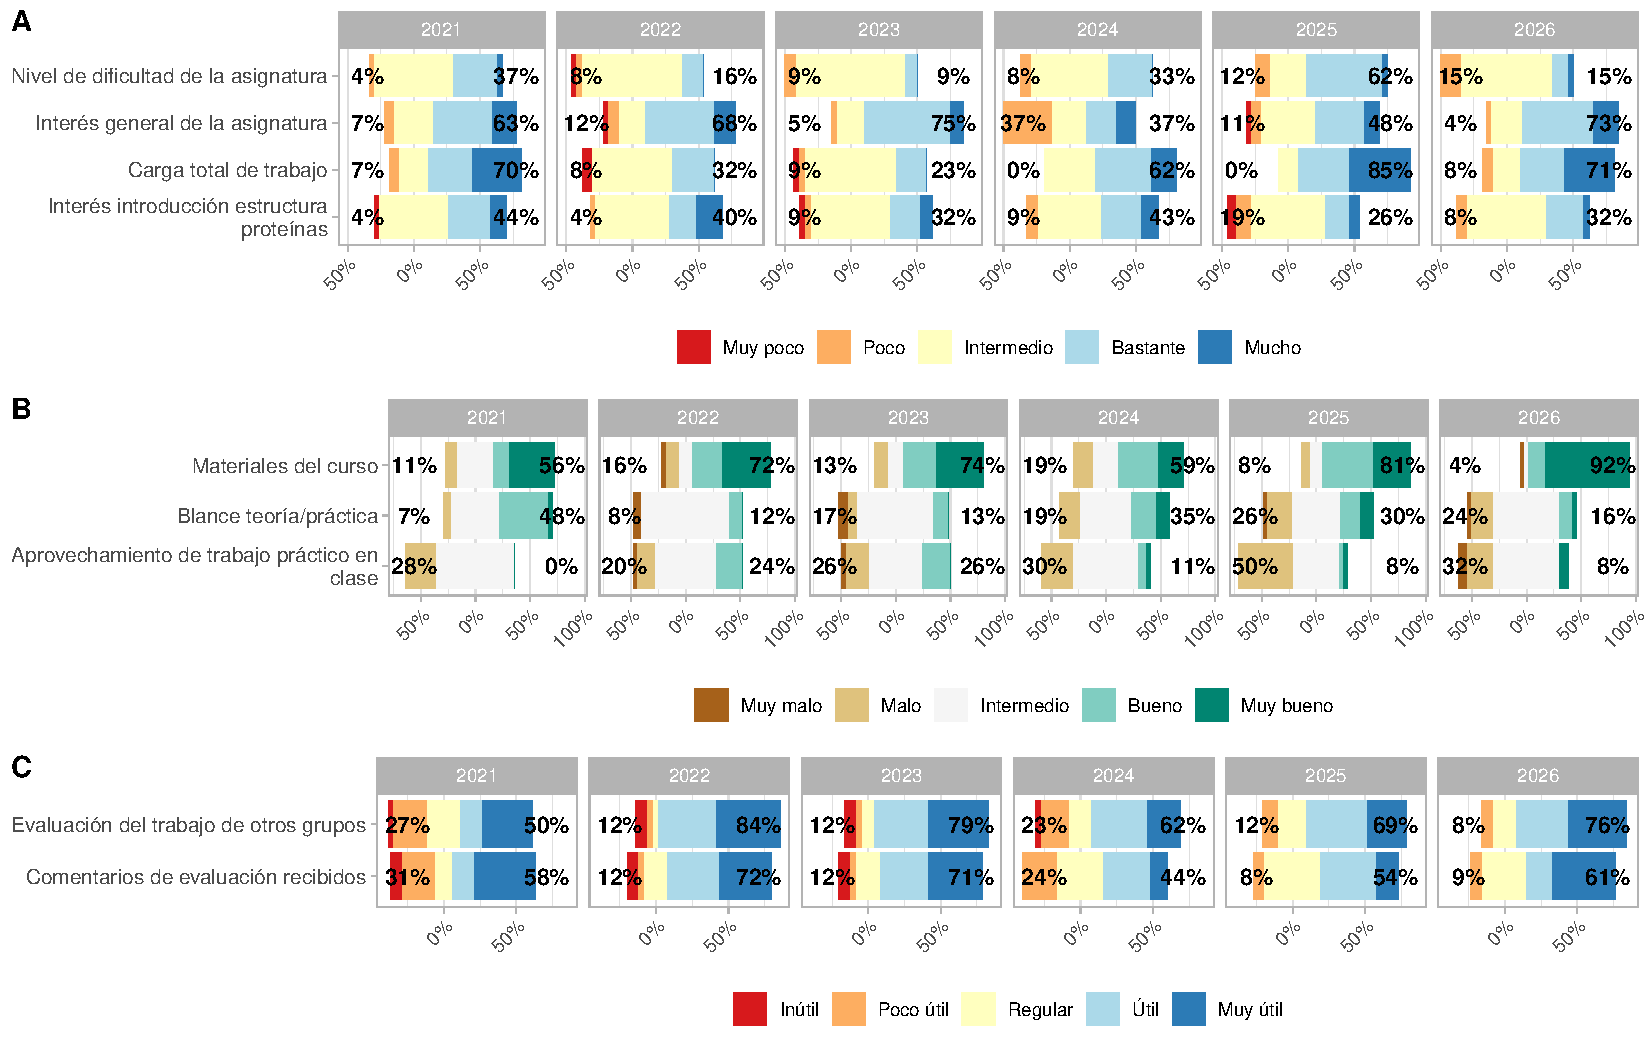
\includegraphics[keepaspectratio]{propuesta_files/figure-pdf/fig-encuestas-1.pdf}}

}

\caption{\label{fig-encuestas}Valoración del alumnado de la asignatura
Bioinformática Estructural entre cursos 2020-2021 y 2025-2026. Se
muestran preguntas seleccionadas entre tres bloques que representan la
valoración general de la asignatura (A), de la metodología docente (B) y
de la evaluación por pares del trabajo práctico (C). Se indica la suma
de las dos valoraciones extremas en cada sentido.}

\end{figure}%

\end{landscape}

En el lado positivo, los materiales del curso reciben sistemáticamente
una valoración alta. Asimismo, la participación en la evaluación por
pares es valorada en general de forma positiva, especialmente por el
aprendizaje derivado de revisar el trabajo de otros compañeros. En los
últimos años se han modificado y ampliado las instrucciones para
orientar mejor la retroalimentación entre iguales, aunque consideramos
que todavía existe margen de mejora en este aspecto.

En conjunto, los resultados sugieren que la asignatura está bien
valorada por su interés, sus materiales y sus actividades de evaluación
formativa, pero que sigue siendo prioritario revisar el volumen de
trabajo y la estructura de las prácticas presenciales para mejorar su
ajuste a la carga docente prevista.

\subsection{Propuesta de mejora: incorporación progresiva de un agente
de IA para facilitar el prendizaje activo en docencia de
bioinformática}\label{propuesta-de-mejora-incorporaciuxf3n-progresiva-de-un-agente-de-ia-para-facilitar-el-prendizaje-activo-en-docencia-de-bioinformuxe1tica}

A partir de la experiencia acumulada en la asignatura, y en particular
con el fin de mejorar el acompañamiento y \emph{feedback} en el trabajo
práctico para reducir la sensación de alta carga de trabajo de los
estudiantes, se propone la incorporación progresiava de un agente de
inteligencia artificial generativa como herramienta de apoyo al
aprendizaje. Esta propuesta responde a una doble necesidad. Por un lado,
mejorar la retroalimentación de forma estructurada y útil durante el
desarrollo de las prácticas, en un contexto en el que el tiempo
disponible para el seguimiento individualizado del alumnado es
necesariamente limitado. Por otro, incorporar de forma explícita una
dimensión crítica en el uso académico de la IAG en el contexto de
aprendizaje basado en proyectos, orientada no a sustituir el
razonamiento del estudiante, sino a reforzar su capacidad de análisis,
revisión y mejora autónoma del trabajo.

La propuesta no se plantea, por tanto, como un sistema de evaluación
automática, sino como un dispositivo de \emph{feedback formativo}
alineado con los resultados de aprendizaje de la asignatura y con varias
competencias transversales del título, entre ellas el razonamiento
crítico, la autorregulación del aprendizaje y el uso razonable y ético
de herramientas basadas en IA. En este sentido, el agente se concibe
como un apoyo intermedio entre la revisión por pares y la valoración
final del profesorado, manteniéndose esta última como referencia
académica definitiva.

\begin{figure}

\centering{

\pandocbounded{\includegraphics[keepaspectratio]{images/ai_copilot.jpg}}

}

\caption{\label{fig-propuestIA}Esquema de implementación secuencial de
la IA como herramienta para proporcionar comentarios de
retroalimentación a los estudiantes.}

\end{figure}%

Tal y como se resume en la Figura~\ref{fig-propuestIA}, durante el curso
2025-26 se llevó a cabo una prueba piloto del uso de la IAG de forma
paralela a la corrección habitual de la práctica \emph{CASP-UAM} de la
asignatura. Como punto de partida, se elaboró un \emph{prompt} inicial
que incluía el enunciado del ejercicio y orientaciones generales sobre
su evaluación. La herramienta seleccionada fue Copilot de Microsoft,
fundamentalmente por motivos prácticos y éticos, ya que su uso en el
marco de la licencia institucional de Microsoft 365 en la UAM
proporciona garantías de privacidad propias del ámbito corporativo y se
ajusta a la normativa de protección de datos (Unión Europea 2016).

El proceso de diseño se desarrolló de forma iterativa y repartida en
varias sesiones, hasta generar una rúbrica analítica suficientemente
estable y consistente (Sección~\ref{sec-anex}). Esta rúbrica permitió
explicitar con mayor precisión los criterios docentes que ya se venían
aplicando en la asignatura, organizándolos en torno a cuatro bloques
---métodos, resultados, conclusiones y formato---, y concretando tanto
las evidencias mínimas esperables como los rasgos propios de un trabajo
excelente. De forma general, la evaluación obtenida con Copilot a partir
de esta rúbrica producía comentarios de retroalimentación muy detallados
y unas calificaciones aproximadas similares a las del profesor.

Sobre la base de esa versión refinada de la rúbrica, se configuró
posteriormente un agente específico de IAG con Microsoft Agent Builder,
denominado \textbf{Evaluador StrBio}, concebido como herramienta
interactiva para proporcionar \emph{feedback} sobre el trabajo en tiempo
casi real. Para su configuración se utilizó un \emph{prompt} específico
que restringía explícitamente el tipo de comentarios y respuestas que el
agente podía generar (Sección~\ref{sec-2anex2}). En particular, se
diseñó para evitar que proporcionara soluciones cerradas, código,
comandos o confirmaciones definitivas, y para que centrara su
intervención en señalar fortalezas, aspectos a mejorar y sugerencias de
revisión, siempre de acuerdo con los criterios de la rúbrica.

Además, durante la fase de configuración se proporcionaron cuatro
trabajos previamente calificados como ejemplos de referencia y
calibración. Una vez ajustado el agente, y con el fin de comprobar su
funcionamiento en un escenario distinto del usado para entrenarlo, se
solicitó la evaluación de otro conjunto de cinco trabajos del mismo
curso. Esta validación permitió obtener tanto un ejemplo representativo
del tipo de \emph{feedback} generado (Sección~\ref{sec-3anex3}) como una
comparación entre las calificaciones aproximadas emitidas por el agente
y las notas asignadas por el profesor (Tabla~\ref{tbl-notas}). Como
puede observarse, las valoraciones del agente son, en general, similares
o ligeramente inferiores a las del profesor, lo que sugiere, por una
parte, que la herramienta tiende a identificar de forma sistemática
aspectos susceptibles de mejora y, por otra, que la revisión final por
parte del docente sigue siendo necesaria.

\begin{longtable}[]{@{}lll@{}}
\caption{Comparación entre las calificaciones aproximadas generadas por
el agente de Copilot y las notas asignadas por el profesor. Se usaron
trabajos correspondientes a grupos distintos a los utilizados como
ejemplo en la configuración y calibración del
agente.}\label{tbl-notas}\tabularnewline
\toprule\noalign{}
Grupo & Nota Agente & Nota Profesor \\
\midrule\noalign{}
\endfirsthead
\toprule\noalign{}
Grupo & Nota Agente & Nota Profesor \\
\midrule\noalign{}
\endhead
\bottomrule\noalign{}
\endlastfoot
1 & 8.5-9.2 & 9.7 \\
2 & 8-8.8 & 8.8 \\
4 & 8.3-9 & 9.2 \\
5 & 7.8-8.8 & 9.25 \\
9 & 8.1-10 & 9.7 \\
\end{longtable}

La implantación prevista para el próximo curso 2026-27 se plantea de
forma gradual y en dos fases. En una primera fase, al inicio de la
asignatura, se proporcionará al alumnado una versión simplificada de la
rúbrica (Tabla~\ref{tbl-rubrica}), elaborada a partir de la versión
completa testada previamente. El objetivo de esta simplificación es
hacer más transparentes los criterios de calidad del proyecto y
facilitar que los estudiantes orienten mejor la planificación y
redacción de su trabajo. En una segunda fase, una vez completado el
proceso de evaluación por pares, se facilitará el acceso al agente, de
modo que cada grupo pueda utilizarlo para revisar y corregir su trabajo
a la luz de los comentarios recibidos. En la sesión final de repaso y
resolución de dudas, que habitualmente coincide en el inicio del proceso
de \emph{peer review} de la práctica CASP-UAM se explicará la actividad
a los estudiantes, indicando que se hará coincidir la finalización de la
revisión por pares con la publicación en Moodle del enlace al agente. Se
comentará el objetivo de su uso y la disponibilidad para comentar, por
correo electrónico o mediante sesiones de tutorías, el feedback recibido
por el agente. Puesto que la práctica CASP-UAM está concebida como
trabajo final de la asignatura y debido a lo apretado del calendario en
una asignatura de solo 3 ECTS, después de compartir el acceso al agente
no quedará tiempo para más sesiones de clases de con los estudiantes,
por lo que es muy importante que en esta sesión final se explique todo
el proceso. Al situar el uso del agente en esta fase final, se minimiza
el efecto de la posible ayuda excesiva que pudiera proporcionar en
etapas tempranas del proceso (\emph{agent spoiler}), asegurando así que
esta actividad no interfiere de forma directa sobre el valor formativo
del trabajo autónomo y de la revisión entre iguales.

\begin{longtable}[]{@{}
  >{\raggedright\arraybackslash}p{(\linewidth - 6\tabcolsep) * \real{0.1857}}
  >{\raggedright\arraybackslash}p{(\linewidth - 6\tabcolsep) * \real{0.0857}}
  >{\raggedright\arraybackslash}p{(\linewidth - 6\tabcolsep) * \real{0.3714}}
  >{\raggedright\arraybackslash}p{(\linewidth - 6\tabcolsep) * \real{0.3571}}@{}}
\caption{Rúbrica resumida para evaluar las prácticas de la asignatura
que se proporcionará a los estudiantes. Se incluye la puntuación de cada
apartado (sobre 10) y una breve descripción de lo que se espera en cada
sección. La rúbrica completa se detalla en el
Sección~\ref{sec-anex}.}\label{tbl-rubrica}\tabularnewline
\toprule\noalign{}
\begin{minipage}[b]{\linewidth}\raggedright
Bloque
\end{minipage} & \begin{minipage}[b]{\linewidth}\raggedright
Puntos
\end{minipage} & \begin{minipage}[b]{\linewidth}\raggedright
Excelente
\end{minipage} & \begin{minipage}[b]{\linewidth}\raggedright
A mejorar
\end{minipage} \\
\midrule\noalign{}
\endfirsthead
\toprule\noalign{}
\begin{minipage}[b]{\linewidth}\raggedright
Bloque
\end{minipage} & \begin{minipage}[b]{\linewidth}\raggedright
Puntos
\end{minipage} & \begin{minipage}[b]{\linewidth}\raggedright
Excelente
\end{minipage} & \begin{minipage}[b]{\linewidth}\raggedright
A mejorar
\end{minipage} \\
\midrule\noalign{}
\endhead
\bottomrule\noalign{}
\endlastfoot
\textbf{Métodos} & 2.0 & Uso de ≥2 métodos de modelado por proteína,
bien justificados y adaptados al problema. Flujo reproducible y
criterios de evaluación de modelos claros; decisiones coherentes (TM,
desorden, oligómeros, plantillas). & Métodos genéricos, poco
justificados o sin adaptación al problema; falta de estrategia clara o
reproducibilidad. \\
\textbf{Resultados} & 3.5 & Comparación rigurosa de modelos (cualitativa
y/o cuantitativa), con figuras (mapas de contacto, superposiciones,
etc.) tablas de métricas comparables (QmeanDisCo, pLDDT, pTM, PAE\ldots)
y figuras informativas y descriptivas de las estructuras. Interpretación
integrada estructural + funcional. & Métricas presentadas sin
interpretación, comparación superficial o inexistente; figuras poco
informativas. Falta de análisis funcional de las estructuras. \\
\textbf{Conclusiones} & 3.0 & Interpretación crítica que integra calidad
estructural, limitaciones, coherencia entre métodos y relevancia
biológica/evolutiva. Selección del mejor modelo bien justificada. &
Conclusiones superficiales, repetitivas o no sustentadas en los
resultados; falta de análisis crítico o justificación. \\
\textbf{Formato} & 1.5 & Documento claro, bien estructurado (tipo
artículo científico), con figuras y tablas integradas y correctamente
referenciadas. & Documento desordenado, difícil de seguir o mal
estructurado; falta de coherencia interna por división de tareas
parcial; pobre integración de figuras y tablas. \\
\end{longtable}

\medskip

Finalmente, con el fin de valorar la conveniencia de una implantación
estable, se incorporarán nuevas preguntas a la encuesta interna de la
asignatura, utilizando la misma escala de Likert empleada hasta ahora (1
= totalmente en desacuerdo, 5 = totalmente de acuerdo):

\begin{enumerate}
\def\labelenumi{\arabic{enumi}.}
\tightlist
\item
  El \emph{feedback} proporcionado por el agente me ha ayudado a mejorar
  mi trabajo.
\item
  Las observaciones del agente están alineadas con los criterios de la
  rúbrica.
\item
  El agente me ha ayudado a identificar errores o aspectos que no había
  considerado.
\item
  El uso del agente me ha permitido ahorrar tiempo en la versión final
  del proyecto.
\item
  El agente proporciona comentarios suficientemente claros como para
  poder mejorar el trabajo.
\item
  El \emph{feedback} del agente es correcto y fiable en términos
  técnicos.
\item
  El agente sirve de ayuda, pero evita dar directamente indicaciones
  claras o respuestas.
\item
  El nivel técnico y de exigencia del agente es apropiado para el nivel
  de la asignatura.
\item
  Habría sido más útil para el aprendizaje tener el agente al principio
  de la asignatura.
\item
  Me gustaría que este tipo de herramienta se utilizara en otras
  asignaturas.
\end{enumerate}

En función de la valoración obtenida, se analizará la viabilidad de
implantar esta propuesta de manera estable y distintas vías para su
consolidación, entre ellas la solicitud de un Proyecto de Innovación
Docente que permita explorar alternativas tecnológicas complementarias.
En este sentido, una posibilidad futura sería comparar el enfoque actual
con herramientas de IA más especializadas en bioinformática o
biomedicina, por ejemplo sistemas orientados a predicción estructural
como \emph{AlphaFold} o \emph{RoseTTAFold}, o incluso modelos biomédicos
de lenguaje de propósito más específico. Sin embargo, en el contexto de
esta asignatura, una especialización excesiva podría desplazar el foco
desde la interpretación crítica hacia la obtención de respuestas cada
vez más resolutivas, alejándose de los objetivos docentes centrados en
la justificación metodológica, el análisis comparado y la discusión
razonada de limitaciones. Por ello, parece especialmente prometedora la
exploración de plataformas diseñadas específicamente para tutoría y
\emph{feedback} educativo ---por ejemplo, entornos como
\textbf{Khanmigo}, \textbf{MagicSchool} o modelos pedagógicamente
afinados como \textbf{LearnLM}---, así como el desarrollo de diseños
híbridos que integren de forma más estrecha la revisión por pares y la
retroalimentación asistida por agente. En esta línea, trabajos recientes
sobre docencia con agentes conversacionales y sobre la combinación de
\emph{peer-review} y apoyo automatizado sugieren que una mejora futura
especialmente interesante no sería solo cambiar de herramienta, sino
refinar el diseño pedagógico de la interacción, de modo que el agente
actúe como segunda capa de andamiaje tras la revisión entre iguales y
antes de la valoración final del profesorado (Sajadi et al. 2024; Chen
et al. 2025). Desde esta perspectiva, una eventual migración desde Agent
Builder a \textbf{Copilot Studio} seguiría siendo una opción
particularmente atractiva, no solo por su mejor integración
institucional y su mayor capacidad de gobernanza, sino también porque
facilitaría experimentar con este tipo de modelos híbridos de
retroalimentación en otras asignaturas del mismo entorno docente.

Precisamente en esta posibilidad de transferencia a otras asignaturas
reside uno de los principales intereses de la propuesta. La elección de
\emph{Bioinformática Estructural} como contexto de aplicación responde a
su pertinencia dentro del Máster en Bioinformática y Biología
Computacional, pero también a su coherencia con una línea docente más
amplia del candidato en asignaturas situadas en la intersección entre
bioquímica, biología molecular, programación y análisis computacional.
Desde esta perspectiva, la propuesta aquí presentada puede entenderse
como un caso de estudio particularmente desarrollado, cuyos principios
metodológicos ---aprendizaje basado en proyectos, evaluación formativa y
apoyo estructurado al trabajo autónomo--- son potencialmente
extrapolables a otras asignaturas del mismo Máster y a materias afines
del grado, como \emph{Herramientas de Programación en Bioquímica y
Biología Molecular} (Grado en Bioquímica). En este sentido, más que una
intervención circunscrita a una asignatura concreta, la experiencia
descrita puede interpretarse como expresión de una línea de innovación
docente susceptible de adaptación a otros contextos en los que confluyen
programación, análisis de datos biológicos y construcción progresiva de
competencias.

\subsection{Conclusiones y perspectivas
futuras}\label{conclusiones-y-perspectivas-futuras}

La motivación de escribir este Proyecto Docente ha sido fundamentalmente
aprovechar la oportunidad para recopilar información sobre la docencia
que se imparte en el contexto de la plaza y la impartida por el
candidato hasta el momento. No hay por tanto ninguna pretensión de
especialización en teoría de la educación universitaria ni en
inteligencia artificial aplicada a la docencia, sino del intento de
reflexionar, desde la propia experiencia académica y docente, sobre qué
conviene enseñar, cómo hacerlo y de qué manera puede evaluarse mejor el
aprendizaje en el contexto específico de esta plaza. En un entorno
social como el actual, marcado por la rápida transformación de las
biociencias, la creciente integración entre análisis computacional e
interpretación biológica y la irrupción de nuevas herramientas
digitales, parece necesario revisar de forma continua la práctica
docente y tratar de orientarla del modo más responsable, riguroso y útil
para los estudiantes.

En conclusión, la propuesta desarrollada en torno a la asignatura
\emph{Bioinformática Estructural}, aunque diseñada para una asignatura
concreta, no debe entenderse como una propuesta cerrada, sino como una
hoja de ruta para recorrer durante los próximos años, modificable en
base a la experiencia. Esta asignatura es un paradigma en el que se
concentran algunos de los retos que caracterizan hoy la enseñanza de la
bioinformática: la heterogeneidad de la formación previa del alumnado,
la necesidad de integrar conocimientos conceptuales y computacionales, y
la conveniencia de promover formas de trabajo más activas, autónomas y
reflexivas. En este sentido, la propuesta presentada aspira sobre todo a
ordenar y mejorar una práctica docente que ya venía evolucionando,
incorporando de forma más explícita elementos de aprendizaje basado en
proyectos, evaluación formativa y uso prudente de herramientas de apoyo
al \emph{feedback}.

Al mismo tiempo, este planteamiento permite dar cierta unidad a una
línea docente más amplia, coherente con la trayectoria del candidato en
asignaturas situadas en la intersección entre bioquímica, biología
molecular, programación y análisis de datos biológicos
(Sección~\ref{sec-yo}). No se trata tanto de afirmar un modelo cerrado o
exportable sin matices, como de reconocer que algunas de las decisiones
metodológicas aquí descritas pueden resultar también útiles en otros
contextos próximos, tanto en asignaturas del propio Máster en
Bioinformática y Biología Computacional como en materias afines del
grado. La experiencia acumulada en docencia de herramientas
computacionales y programación aplicada sugiere que varias de estas
estrategias pueden adaptarse con sentido a otros entornos en los que el
aprendizaje dependa de la resolución de problemas, del desarrollo
progresivo de competencias o de la necesidad de acompañar de forma más
eficaz el trabajo autónomo del estudiante.

En última instancia, el propósito de este Proyecto Docente es proponer
una forma de trabajo que trate de responder con seriedad a las
exigencias del entorno académico actual sin perder de vista que enseñar
en la universidad sigue siendo, ante todo, una tarea de responsabilidad
intelectual y formativa. Si la investigación obliga a actualizar
conocimientos y métodos de manera constante, la docencia exige además
pensar cómo trasladar esa complejidad al aula de forma comprensible,
exigente y estimulante. Desde esta convicción, la formación
universitaria no debería orientarse únicamente a la adquisición de los
conocimientos y herramientas hoy disponibles, sino también al desarrollo
de la madurez académica, la capacidad crítica y la flexibilidad
intelectual necesarias para seguir aprendiendo y adaptarse a los
conocimientos, métodos y tecnologías que inevitablemente surgirán en el
futuro. En este sentido, este proyecto pretende contribuir modestamente
a mejorar la calidad del aprendizaje en el ámbito de la bioinformática y
de las biociencias moleculares, entendiendo la innovación docente no
como un fin en sí mismo, sino como una consecuencia natural del esfuerzo
por enseñar mejor y por formar estudiantes capaces de desenvolverse con
autonomía, rigor y criterio propio en un contexto científico y
profesional en transformación permanente.

\bookmarksetup{startatroot}

\chapter{Referencias
bibliográficas}\label{referencias-bibliogruxe1ficas}

\protect\phantomsection\label{refs}
\begin{CSLReferences}{1}{1}
\bibitem[\citeproctext]{ref-alcubilla2026}
Alcubilla, Arnaldo. 2026. \emph{Código de Universidades}. CRUE.
\url{https://www.boe.es/biblioteca_juridica/codigos/codigo.php?id=133}.

\bibitem[\citeproctext]{ref-attwood2019}
Attwood, Teresa K, Sarah Blackford, Michelle D Brazas, Angela Davies,
and Maria Victoria Schneider. 2019. {``A Global Perspective on Evolving
Bioinformatics and Data Science Training Needs.''} \emph{Briefings in
Bioinformatics} 20 (2): 398--404.
\url{https://doi.org/10.1093/bib/bbx100}.

\bibitem[\citeproctext]{ref-cano2015}
Cano, Elena. 2015. {``Las Rúbricas Como Instrumento de Evaluación de
Competencias En Educación Superior: ¿Uso o Abuso?''} \emph{Profesorado.
Revista de Currículum y Formación Del Profesorado} 19 (2).
\url{https://www.ugr.es/~recfpro/rev192COL2.pdf}.

\bibitem[\citeproctext]{ref-chen_generative_2025}
Chen, Shih-Yeh, Wei-Cheng Chen, and Chin-Feng Lai. 2025. {``Generative
{AI} as a Reflective Scaffold in a {UAV}-Based {STEM} Project: {A}
Mixed-Methods Study on Students' Higher-Order Thinking and Cognitive
Transformation.''} \emph{Education and Information Technologies} 30
(17): 24787--814. \url{https://doi.org/10.1007/s10639-025-13758-4}.

\bibitem[\citeproctext]{ref-crue2019}
Conferencia de Rectores de las Universidades Españolas (CRUE). 2019.
\emph{La universidad como ascensor social}. CRUE Universidades
Españolas.
\url{https://www.crue.org/wp-content/uploads/2020/02/Cap.-5-Ascensor-social.pdf}.

\bibitem[\citeproctext]{ref-cotton_beyond_2026}
Cotton, Peter A., and Debby R. E. Cotton. 2026. {``Beyond {ChatGPT}: A
Review of the Use of {AI} Tools in Biological Education.''}
\emph{Journal of Biological Education} 0 (0): 1--25.
\url{https://doi.org/10.1080/00219266.2026.2628797}.

\bibitem[\citeproctext]{ref-cruzargudo2024}
Cruz Argudo, Francisco, Ismael García Varea, Juan A. Martínez Carrascal,
et al. 2024. \emph{La Inteligencia Artificial Generativa En La Docencia
Universitaria: Oportunidades, Desafíos y Recomendaciones}.
\url{https://www.crue.org/wp-content/uploads/2024/03/Crue-Digitalizacion_IA-Generativa.pdf}.

\bibitem[\citeproctext]{ref-alma991007757245904211}
Cuervas-Mons Martínez, Valentín. 2018. \emph{Cincuenta años de la
Facultad de Medicina de la UAM: Quid ultra faciam}. Fundación Teófilo
Hernando.

\bibitem[\citeproctext]{ref-fundacion_cyd_uso_2026}
CYD, Fundación. 2026. \emph{Uso y Percepción de La {IA} En El Entorno
Universitario {II}}.
\url{https://www.fundacioncyd.org/publicaciones-cyd/uso-y-percepcion-de-la-ia-en-el-entorno-universitario-ii/}.

\bibitem[\citeproctext]{ref-delcher2025}
Delcher, Haley A., Enas S. Alsatari, Adeyeye I. Haastrup, et al. 2025.
{``Using ChatGPT as a Tool for Training Nonprogrammers to Generate
Genomic Sequence Analysis Code.''} \emph{Biochemistry and Molecular
Biology Education} 53 (4): 433--44.
\url{https://doi.org/10.1002/bmb.21899}.

\bibitem[\citeproctext]{ref-directorate-generalforeducation2026}
Directorate-General for Education, Youth, Sport and Culture (European
Commission). 2026. \emph{Guidelines on the Ethical Use of Artificial
Intelligence and Data in Teaching and Learning for Educators}.
\url{https://doi.org/10.2766/7967834}.

\bibitem[\citeproctext]{ref-europeancommission2015}
European Commission. 2015. \emph{ECTS Users{'} Guide 2015}.
\url{https://doi.org/10.2766/763090}.

\bibitem[\citeproctext]{ref-europeanparliamentaryresearchservice2021}
European Parliamentary Research Service. 2021. \emph{The European
Education Area and the 2030 Strategic Framework for Education and
Training}.
\url{https://www.europarl.europa.eu/RegData/etudes/BRIE/2021/690630/EPRS_BRI(2021)690630_EN.pdf}.

\bibitem[\citeproctext]{ref-feldon2011}
Feldon, David F., James Peugh, Briana E. Timmerman, et al. 2011.
{``Graduate Students{'} Teaching Experiences Improve Their
Methodological Research Skills.''} \emph{Science} 333 (6045): 1037--39.
\url{https://doi.org/10.1126/science.1204109}.

\bibitem[\citeproctext]{ref-fernandezmadinabeitia2020}
Fernández Fernández, Idoia, and Alba Madinabeitia Ezkurra. 2020. {``La
Transformación Docente de La Universidad a Veinte Años de Bolonia:
Balance y Claves Para Un Futuro Por Definir.''} \emph{Profesorado.
Revista de Currículum y Formación Del Profesorado} 24 (2).
\url{https://doi.org/10.30827/profesorado.v24i2.15149}.

\bibitem[\citeproctext]{ref-frydenberg2025}
Frydenberg, Mark, Anqi Xu, and Jennifer Xu. 2025. {``Student Perceptions
of Learning Through Original and AI-Generated Python Programs from a
Software Quality Perspective.''} \emph{Information Systems Education
Journal} 25 (4): 34--56. \url{https://doi.org/10.62273/DVNQ9288}.

\bibitem[\citeproctext]{ref-gooblar_missing_2019}
Gooblar, David. 2019. \emph{The {Missing} {Course}: {Everything} {They}
{Never} {Taught} {You} about {College} {Teaching}}. Harvard University
Press. \url{https://www.hup.harvard.edu/books/9780674260382}.

\bibitem[\citeproctext]{ref-hernandez2025}
Hernández Armenteros, Juan, and José Antonio Pérez García. 2025.
\emph{La Universidad Española En Cifras 2023-2024}. XV edición. CRUE
Universidades Españolas.
\url{https://www.crue.org/wp-content/uploads/2026/01/UEC_2023-2024.pdf}.

\bibitem[\citeproctext]{ref-iglesiassoilan2024}
Iglesias-Soilán, Manuel, Irene Sánchez-San-José, Andrés Cano-Maganto,
and Claudia Carretero-Peinado. 2024. {``Lección magistral interactiva:
una metodología universitaria asequible y eficiente.''} \emph{Revista
Colombiana de Educación}, no. 90 (January): 283--303.
\url{https://doi.org/10.17227/rce.num90-15889}.

\bibitem[\citeproctext]{ref-juxe1comeayala2025}
Jácome Ayala, Paulina Johanna, and Marco Antonio Checa Cabrera. 2025.
{``Impacto de la Inteligencia Artificial Generativa en el aprendizaje de
estudiantes de Desarrollo de Software: Impacto de la Inteligencia
Artificial Generativa en el aprendizaje de estudiantes de Desarrollo de
Software.''} \emph{HOLOPRAXIS: Revista de Ciencia, Tecnología e
Innovación} 9 (2): 366--85.
\url{https://dialnet.unirioja.es/servlet/articulo?codigo=10471120}.

\bibitem[\citeproctext]{ref-johnson2018}
Johnson, David W., and Roger T. Johnson. 2018. {``Cooperative Learning:
The Foundation for Active Learning.''} In \emph{Active Learning---Beyond
the Future}, edited by Sílvio Manuel Brito. IntechOpen.
\url{https://doi.org/10.5772/intechopen.81086}.

\bibitem[\citeproctext]{ref-kuxf6peczi-buxf3cz2025}
Köpeczi-Bócz, Tamás. 2025. \emph{New Paradigms of learning}.
\url{https://zemplenimuzsa.hu/konyveink/}.

\bibitem[\citeproctext]{ref-krajcik2005}
Krajcik, Joseph S., and Phyllis C. Blumenfeld. 2005. \emph{Project-Based
Learning}. Edited by R. Keith Sawyer. Cambridge University Press.
\url{https://doi.org/10.1017/CBO9780511816833.020}.

\bibitem[\citeproctext]{ref-liu_oportunidades_2023}
Liu, Bosen Lily, Diana Morales, Jaime Félix Roser-Chinchilla, et al.
2023. \emph{Oportunidades y Desafíos de La Era de La Inteligencia
Artificial Para La Educación Superior: Una Introducción Para Los Actores
de La Educación Superior}. Programme and meeting document. Edited by
UNESCO International Institute for Higher Education in Latin America and
the Caribbean. UNESCO.
\url{https://unesdoc.unesco.org/ark:/48223/pf0000386670_spa}.

\bibitem[\citeproctext]{ref-luxf3pezmelgarejo2019}
López Melgarejo, Alba María. 2019. {``La Junta Nacional contra el
analfabetismo (1950-1970): un análisis documental.''} \emph{Educatio
siglo XXI: Revista de la Facultad de Educación} 37 (2): 267--86.
\url{https://dialnet.unirioja.es/servlet/articulo?codigo=7095136}.

\bibitem[\citeproctext]{ref-luxf3pezpastor2009}
López Pastor, V. M. 2009. \emph{Evaluación formativa y compartida en
Educación Superior : propuestas, técnicas, instrumentos y experiencias}.
\url{http://www.digitaliapublishing.com/a/29006/evaluacion-formativa-y-compartida-en-educacion-superior---propuestas--tecnicas--instrumentos-y-experiencias}.

\bibitem[\citeproctext]{ref-meyer2021}
Meyer, Cosima. 2021. {``Bringing the World to the Classroom: Teaching
Statistics and Programming in a Project-Based Setting.''} \emph{PS:
Political Science \& Politics}, ahead of print.
\url{https://doi.org/10.1017/S1049096521001104}.

\bibitem[\citeproctext]{ref-miao2024}
Miao, Fengchun, and Wayne Holmes. 2024. \emph{Guía para el uso de IA
generativa en educación e investigación}. Guidance for generative AI in
education and research. Organización de las Naciones Unidas para la
Educación, la Ciencia y la Cultura (UNESCO).
\url{https://unesdoc.unesco.org/ark:/48223/pf0000389227}.

\bibitem[\citeproctext]{ref-bologna1999}
Ministros europeos de Educación. 1999. \emph{Declaración de bolonia:
Espacio europeo de educación superior}. Bolonia, Italia.
\url{https://ehea.info/media.ehea.info/file/Ministerial_conferences/06/0/1999_Bologna_Declaration_Spanish_553060.pdf}.

\bibitem[\citeproctext]{ref-morellmoll2004}
Morell Moll, Teresa Author. 2004. \emph{La Interacción En La Clase
Magistral}. Publicaciones de la Universidad de Alicante.

\bibitem[\citeproctext]{ref-organisationforeconomicco-operationanddevelopment2024}
Organisation for Economic Co-operation and Development. 2024.
\emph{Education at a Glance 2024: OECD Indicators}. {OECD Publishing}.
\url{https://doi.org/10.1787/c00cad36-en}.

\bibitem[\citeproctext]{ref-petersen2020}
Petersen, Christina I., Paul Baepler, Al Beitz, et al. 2020. {``The
Tyranny of Content: {``}Content Coverage{''} as a Barrier to
Evidence-Based Teaching Approaches and Ways to Overcome It.''}
\emph{CBE{\textemdash}Life Sciences Education} 19 (2): ar17.
\url{https://doi.org/10.1187/cbe.19-04-0079}.

\bibitem[\citeproctext]{ref-pineda-alfonso2020}
Pineda-Alfonso, José Antonio, and Olga María Duarte Piña. 2020. {``Las
Concepciones Pedagógicas Del Profesorado Universitario: Un Punto de
Partida Para El Cambio Docente.''} \emph{Educación XX1} 23 (2): 95118.
\url{https://doi.org/10.5944/educXX1.25409}.

\bibitem[\citeproctext]{ref-ramsden_learning_2003}
Ramsden, Paul. 2003. \emph{Learning to Teach in Higher Education}. 2nd
ed. RoutledgeFalmer.

\bibitem[\citeproctext]{ref-ruizmartuxedn2020}
Ruiz Martín, Héctor. 2020. \emph{¿Cómo Aprendemos?} Grao.

\bibitem[\citeproctext]{ref-sajadi_harnessing_nodate}
Sajadi, Susan, Mark Huerta, Olivia Ryan, and Katie Drinkwater. 2024.
\emph{Harnessing {Generative} {AI} to {Enhance} {Feedback} {Quality} in
{Peer} {Evaluations} Within {Project}-{Based} {Learning} {Contexts}}.

\bibitem[\citeproctext]{ref-sajadieh}
Sajadieh, Sha, Loredana Fattorini, Raymond Perrault, et al. 2026.
\emph{The 2026 AI Index Report}.

\bibitem[\citeproctext]{ref-suxe1nchez2008}
Sánchez, Primitivo. 2008. \emph{Planificar La Formación En El Espacio
Europeo de Educación Superior Títulos Oficiales y Materias}. ICE de la
Universidad Complutense.

\bibitem[\citeproctext]{ref-shue2023}
Shue, Evelyn, Li Liu, Bingxin Li, Zifeng Feng, Xin Li, and Gangqing Hu.
2023. {``Empowering Beginners in Bioinformatics with ChatGPT.''}
\emph{Quantitative Biology} 11 (2): 105--8.
\url{https://doi.org/10.15302/J-QB-023-0327}.

\bibitem[\citeproctext]{ref-suresh2025}
Suresh, Divya, Melis Dilek, Aliye Karabulut-Ilgu, Evrim Baran, and
Michael Kimber. 2025. {``GENERATIVE AI IN LEARNING DESIGN PRACTICE:
BUILDING AN ONLINE COURSE FOR BIOMEDICAL SCIENCES RESEARCH PROGRAMS.''}
\emph{International Journal of Designs for Learning} 16 (2): 244--65.
\url{https://doi.org/10.14434/ijdl.v16i2.41995}.

\bibitem[\citeproctext]{ref-teufel_teaching_2026}
Teufel, Ashley I., and David A. Liberles. 2026. {``Teaching
Bioinformatics with Generative {AI}: Judgment, Uncertainty, and
Responsibility.''} \emph{Journal of Microbiology \& Biology Education}
27 (2): e0033125. \url{https://doi.org/10.1128/jmbe.00331-25}.

\bibitem[\citeproctext]{ref-theobald2020}
Theobald, Elli J., Mariah J. Hill, Elisa Tran, et al. 2020. {``Active
Learning Narrows Achievement Gaps for Underrepresented Students in
Undergraduate Science, Technology, Engineering, and Math.''}
\emph{Proceedings of the National Academy of Sciences} 117 (12):
6476--83. \url{https://doi.org/10.1073/pnas.1916903117}.

\bibitem[\citeproctext]{ref-torres2023}
Torres, Cinta Gallent, Alfredo Zapata González, and José Luis Ortego
Hernando. 2023. {``El impacto de la inteligencia artificial generativa
en educación superior: una mirada desde la ética y la integridad
académica.''} \emph{RELIEVE - Revista Electrónica de Investigación y
Evaluación Educativa} 29 (2).
\url{https://doi.org/10.30827/relieve.v29i2.29134}.

\bibitem[\citeproctext]{ref-uniuxf3neuropea2016}
Unión Europea. 2016. {``Reglamento (UE) 2016/679 Del Parlamento Europeo
y Del Consejo, de 27 de Abril de 2016, Relativo a La Protección de Las
Personas Físicas En Lo Que Respecta Al Tratamiento de Datos Personales y
a La Libre Circulación de Estos Datos (Reglamento General de Protección
de Datos, RGPD).''} \emph{Diario Oficial de La Unión Europea} L 119
(April): 1--88. \url{https://eur-lex.europa.eu/eli/reg/2016/679/oj}.

\bibitem[\citeproctext]{ref-valverde-berrocoso2022}
Valverde-Berrocoso, Jesús, Jesús Acevedo-Borrega, and Mario
Cerezo-Pizarro. 2022. {``Educational Technology and Student Performance:
A Systematic Review.''} \emph{Frontiers in Education} 7: 916502.
\url{https://doi.org/10.3389/feduc.2022.916502}.

\bibitem[\citeproctext]{ref-wang2024}
Wang, Jinge, Zien Cheng, Qiuming Yao, Li Liu, Dong Xu, and Gangqing Hu.
2024. {``Bioinformatics and Biomedical Informatics with ChatGPT: Year
One Review.''} \emph{Quantitative Biology} 12 (4): 345--59.
\url{https://doi.org/10.1002/qub2.67}.

\end{CSLReferences}

\bookmarksetup{startatroot}

\chapter{Anexos}\label{anexos}

\setcounter{secnumdepth}{0}

\section{Anexo I: Rúbrica detallada de evaluación de
prácticas}\label{sec-anex}

\subsubsection{1. Estructura de la
evaluación}\label{estructura-de-la-evaluaciuxf3n}

La calificación es \textbf{sobre 10 puntos}, distribuida en cuatro
bloques:

\begin{itemize}
\item
  \textbf{Métodos:} 2.0 puntos
\item
  \textbf{Resultados:} 3.5 puntos
\item
  \textbf{Conclusiones:} 3.0 puntos
\item
  \textbf{Formato (documento científico):} 1.5 puntos
\end{itemize}

\textbf{Nota final = Métodos + Resultados + Conclusiones + Formato}

\subsubsection{\texorpdfstring{2. Enunciado general:
\url{https://strbio.github.io/casp.html}}{2. Enunciado general: https://strbio.github.io/casp.html}}\label{enunciado-general-httpsstrbio.github.iocasp.html}

Este ejercicio es tipo \textbf{CASP}. Debéis modelar \textbf{al menos
tres proteínas} y, para cada una de ellas:

\begin{itemize}
\item
  recopilar de bases de datos o publicaciones información previa
  relevante:

  \begin{itemize}
  \tightlist
  \item
    oligomerización
  \item
    ligandos / cofactores
  \item
    regiones transmembrana
  \item
    regiones desordenadas
  \item
    disponibilidad de plantillas y/o homólogos estructurales
  \end{itemize}
\item
  usar \textbf{más de un protocolo de modelado}
\item
  \textbf{justificar la elección de métodos}
\item
  seleccionar el mejor modelo
\item
  describir la estructura, incluyendo mapas de contacto, estructura
  secundaria, motivos, dominios, etc.
\item
  evaluar las estructuras funcional y/o evolutivamente
\end{itemize}

Los modelos deben evaluarse con métricas como:

\begin{itemize}
\item
  \textbf{pLDDT}
\item
  \textbf{pTM / ipTM}
\item
  \textbf{PAE}
\item
  y/o validaciones independientes (\textbf{QMEANDisCo, VoroMQA,
  MolProbity, Ramachandran}, etc.)
\end{itemize}

La comparación entre modelos debe incluir:

\begin{itemize}
\item
  comparación estructural
\item
  comparación cualitativa y/o cuantitativa
\item
  interpretación estructural
\item
  interpretación funcional o evolutiva cuando proceda
\end{itemize}

\subsubsection{A) Métodos --- 2.0 puntos}\label{a-muxe9todos-2.0-puntos}

\subsubsection{Qué se evalúa}\label{quuxe9-se-evaluxfaa}

Diseño computacional, adecuación de los protocolos al problema
estructural y claridad metodológica.

\subsubsection{Evidencias mínimas}\label{evidencias-muxednimas}

\begin{itemize}
\item
  Uso de \textbf{\textgreater1 protocolo de modelado por proteína}
\item
  Justificación del protocolo de modelado \textbf{por proteína}
\item
  Explicación de los criterios de evaluación de modelos
\item
  Descripción del flujo de trabajo de forma reproducible
\item
  Consideración, cuando proceda, de:

  \begin{itemize}
  \tightlist
  \item
    monómero vs complejo
  \item
    regiones TM/desordenadas
  \item
    ligandos/cofactores
  \item
    disponibilidad de plantillas
  \item
    nivel de conservación/divergencia
  \end{itemize}
\end{itemize}

\subsubsection{Qué debe valorarse
especialmente}\label{quuxe9-debe-valorarse-especialmente}

\begin{itemize}
\item
  Que la elección de protocolos \textbf{no sea genérica}, sino adaptada
  al problema:

  \begin{itemize}
  \tightlist
  \item
    proteína con regiones TM
  \item
    proteína desordenada
  \item
    oligómero
  \item
    proteína con buenos \emph{templates}
  \item
    proteína sin homólogos estructurales claros
  \end{itemize}
\item
  Que el alumnado explique \textbf{por qué compara esos métodos
  concretos} en ese caso
\item
  Que la descripción de la metodología permita \textbf{reproducir} los
  resultados
\end{itemize}

\subsubsection{Puntuación orientativa}\label{puntuaciuxf3n-orientativa}

\begin{itemize}
\item
  \textbf{2.0 (Excelente):} método detallado, bien justificado para cada
  proteína, con decisiones coherentes respecto a
  TM/desorden/oligomería/plantillas y criterios de evaluación bien
  definidos. Introducen el uso de scripts o pipelines para automatizar
  parcialmente el proceso.
\item
  \textbf{1.6 (Bien):} metodología correcta y completa, con
  justificación presente pero algo general. No consta el uso de scripts.
\item
  \textbf{1.2 (Aceptable):} describe procedimientos y herramientas, pero
  sin justificar adecuadamente decisiones clave.
\item
  \textbf{≤0.8 (Insuficiente):} falta estrategia clara o evidencias
  metodológicas significativas.
\end{itemize}

\subsubsection{B) Resultados --- 3.5
puntos}\label{b-resultados-3.5-puntos}

\subsubsection{Qué se evalúa}\label{quuxe9-se-evaluxfaa-1}

Calidad, completitud e integración crítica de las evidencias obtenidas
durante el modelado y la comparación estructural.

\subsubsection{Evidencias mínimas}\label{evidencias-muxednimas-1}

\subsubsection{1. Presentación comparativa de
modelos}\label{presentaciuxf3n-comparativa-de-modelos}

\begin{itemize}
\tightlist
\item
  Tabla(s) comparativas por proteína y por modelo con:

  \begin{itemize}
  \tightlist
  \item
    pLDDT
  \item
    pTM / ipTM
  \item
    PAE
  \item
    métricas independientes
  \end{itemize}
\item
  Selección razonada del mejor modelo por proteína
\end{itemize}

\subsubsection{2. Comparación estructural
(obligatoria)}\label{comparaciuxf3n-estructural-obligatoria}

La comparación estructural entre modelos es \textbf{obligatoria}, pero
puede realizarse de dos formas:

\begin{itemize}
\item
  \textbf{Comparación cuantitativa}, mediante RMSD u otras métricas
  estructurales, y
\item
  \textbf{Comparación cualitativa detallada}, incluyendo descripción
  narrativa y mapas de contacto. Excepcionalmente puede suplir la
  comparación cualitativa, siempre que esté suficientemente
  desarrollada.
\end{itemize}

Una comparación cualitativa se considerará suficiente cuando identifique
y discuta de forma clara la mayoría de los siguientes aspectos:

\begin{itemize}
\item
  regiones conservadas y divergentes
\item
  motivos, dominios o subestructuras relevantes
\item
  regiones flexibles o desordenadas
\item
  diferencias entre monómero y complejo, si aplica
\item
  posibles implicaciones funcionales o evolutivas
\end{itemize}

\begin{quote}
La comparación cuantitativa (por ejemplo, RMSD) \textbf{se valora
positivamente}, pero \textbf{no es imprescindible} para alcanzar una
valoración alta si existe una comparación estructural cualitativa
suficientemente profunda, rigurosa y bien argumentada. La máxima
valoración requiere las dos cosas.
\end{quote}

\subsubsection{3. Calidad informativa de figuras
estructurales}\label{calidad-informativa-de-figuras-estructurales}

Se valorará la comparación de mapas de contacto entre los diferentes
modelos.\\
Las figuras de PyMOL / ChimeraX / Mol* / similares deben ser
\textbf{analíticas}, no meramente decorativas.

Se valorará que:

\begin{itemize}
\item
  reflejen el resultado que se discute
\item
  estén relacionadas con una pregunta concreta
\item
  destaquen regiones relevantes
\item
  incluyan una leyenda o explicación suficiente
\item
  permitan interpretar:

  \begin{itemize}
  \tightlist
  \item
    similitud/diferencia estructural
  \item
    regiones conservadas o divergentes
  \item
    localización de dominios, TM, interfaces o regiones flexibles
  \item
    relación con la calidad del modelo
  \end{itemize}
\end{itemize}

\begin{quote}
No se considerarán de alto valor evaluativo las figuras que solo
``muestren la proteína'' o ``muestren una superposición'' sin aportar
información adicional o sin sostener explícitamente la interpretación
del texto.
\end{quote}

\subsubsection{4. Similitud estructural, conservación y contexto
biológico}\label{similitud-estructural-conservaciuxf3n-y-contexto-bioluxf3gico}

Se valorará explícitamente la incorporación de análisis de:

\begin{itemize}
\item
  similitud estructural con estructuras conocidas
\item
  conservación estructural
\item
  búsqueda de análogos estructurales
\item
  anotación funcional basada en la estructura
\end{itemize}

Ejemplos de herramientas posibles (no obligatorias):

\begin{itemize}
\item
  Foldseek
\item
  DALI
\item
  FoldTree
\item
  FoldMason
\item
  búsquedas estructurales equivalentes
\item
  comparación con estructuras experimentales relevantes
\end{itemize}

\subsubsection{5. Integración e interpretación de
resultados}\label{integraciuxf3n-e-interpretaciuxf3n-de-resultados}

El bloque de resultados debe mostrar no solo métricas, sino también
\textbf{lectura crítica} de lo que significan:

\begin{itemize}
\item
  convergencia o divergencia entre métodos
\item
  qué partes del modelo son fiables y cuáles no
\item
  cuándo un buen score no basta
\item
  cuándo una plantilla experimental aporta mayor valor biológico que una
  predicción cerrada
\end{itemize}

\subsubsection{Qué debe valorarse
especialmente}\label{quuxe9-debe-valorarse-especialmente-1}

\begin{itemize}
\item
  La \textbf{integración} entre métricas, comparación estructural,
  figuras e interpretación
\item
  La capacidad de distinguir entre:

  \begin{itemize}
  \tightlist
  \item
    ``modelo geométricamente correcto''
  \item
    ``modelo biológicamente útil''
  \item
    ``modelo con soporte funcional o evolutivo''
  \end{itemize}
\item
  Que la comparación no se limite a una lista de scores
\end{itemize}

\subsubsection{Puntuación
orientativa}\label{puntuaciuxf3n-orientativa-1}

\begin{itemize}
\item
  \textbf{3.5 (Excelente):} resultados completos, comparativos e
  integrados. Hay tablas claras y comparación estructural rigurosa. Esto
  puede lograrse:

  \begin{itemize}
  \tightlist
  \item
    mediante combinación de comparación cuantitativa y cualitativa, o
  \item
    mediante una comparación cualitativa especialmente sólida y
    detallada, aunque no se haya incluido RMSD.\\
    Además, las figuras son informativas y existe análisis de similitud
    estructural / conservación / anotación funcional cuando procede.
  \end{itemize}
\item
  \textbf{2.5-3 (Bien):} resultados sólidos y bien presentados, con
  comparación estructural suficiente, pero falta profundidad en alguno
  de estos aspectos:

  \begin{itemize}
  \tightlist
  \item
    integración funcional/evolutiva
  \item
    valor informativo de las figuras
  \item
    sistematicidad en la comparación
  \item
    o uso/interpretación de métricas cuantitativas
  \end{itemize}
\item
  \textbf{1.5-2.5 (Aceptable):} se presentan modelos y métricas, pero
  con comparación estructural limitada o superficial. La descripción
  comparativa existe, pero no permite sostener con claridad la selección
  del mejor modelo o la interpretación estructural.
\item
  \textbf{≤1.4 (Insuficiente):} evidencia escasa, fragmentaria o
  incoherente; predominan descripciones sin verdadera comparación
  estructural ni integración.
\end{itemize}

\subsubsection{Penalizaciones o rebajas cualitativas dentro del
bloque}\label{penalizaciones-o-rebajas-cualitativas-dentro-del-bloque}

Deben bajar la puntuación de \textbf{Resultados} los siguientes
problemas:

\begin{itemize}
\item
  figuras finales de superposición \textbf{decorativas} o poco
  informativas
\item
  ausencia de análisis de similitud estructural/conservación cuando
  habría sido relevante
\item
  falta de interpretación funcional basada en la estructura
\item
  comparación entre modelos basada casi exclusivamente en scores sin
  discutir su significado estructural
\item
  selección del ``mejor modelo'' sin criterio explícito
\item
  comparación visual muy superficial, incluso aunque exista RMSD
\end{itemize}

\subsubsection{C) Conclusiones --- 3.0
puntos}\label{c-conclusiones-3.0-puntos}

\subsubsection{Qué se evalúa}\label{quuxe9-se-evaluxfaa-2}

Interpretación estructural, solidez del razonamiento y capacidad de
síntesis.

\subsubsection{Evidencias mínimas}\label{evidencias-muxednimas-2}

\begin{itemize}
\item
  Selección razonada del mejor modelo por proteína
\item
  Discusión de:

  \begin{itemize}
  \tightlist
  \item
    incertidumbre (pLDDT bajo, PAE alto, regiones flexibles)
  \item
    limitaciones metodológicas
  \item
    convergencia o discrepancia entre métodos
  \end{itemize}
\item
  Interpretación estructural basada en:

  \begin{itemize}
  \tightlist
  \item
    métricas de calidad
  \item
    comparación entre modelos
  \item
    contexto funcional o evolutivo
  \end{itemize}
\end{itemize}

\subsubsection{Qué debe valorarse
especialmente}\label{quuxe9-debe-valorarse-especialmente-2}

\begin{itemize}
\item
  Que las conclusiones no repitan simplemente los resultados
\item
  Que integren:

  \begin{itemize}
  \tightlist
  \item
    calidad del modelo
  \item
    utilidad biológica
  \item
    limitaciones
  \item
    posibles pasos siguientes
  \end{itemize}
\item
  Que distingan entre:

  \begin{itemize}
  \tightlist
  \item
    proteína bien resuelta
  \item
    proteína de dificultad intermedia
  \item
    proteína no modelable con confianza
  \end{itemize}
\end{itemize}

\subsubsection{Puntuación
orientativa}\label{puntuaciuxf3n-orientativa-2}

\begin{itemize}
\item
  \textbf{3.0 (Excelente):} conclusiones sólidas, críticas y bien
  sustentadas; integran calidad del modelo, interpretación estructural y
  relevancia biológica.
\item
  \textbf{2.5-3 (Bien):} interpretación correcta, aunque algo menos
  profunda o menos integradora.
\item
  \textbf{1.5-2.5 (Aceptable):} conclusiones superficiales o poco
  conectadas con la evidencia estructural.
\item
  \textbf{≤1.2 (Insuficiente):} conclusiones no sustentadas o
  excesivamente genéricas.
\end{itemize}

\subsubsection{D) Formato (documento científico) --- 1.5
puntos}\label{d-formato-documento-cientuxedfico-1.5-puntos}

\subsubsection{Qué se evalúa}\label{quuxe9-se-evaluxfaa-3}

Calidad del informe, claridad expositiva y utilidad del documento como
trabajo científico.

\subsubsection{Requisitos mínimos}\label{requisitos-muxednimos}

\begin{itemize}
\item
  Objetivo general y, preferiblemente, objetivo por proteína
\item
  Secciones claras:

  \begin{itemize}
  \tightlist
  \item
    Métodos
  \item
    Resultados
  \item
    Conclusiones
  \end{itemize}
\item
  Figuras y tablas con:

  \begin{itemize}
  \tightlist
  \item
    título
  \item
    pie informativo
  \end{itemize}
\item
  Referencias homogéneas:

  \begin{itemize}
  \tightlist
  \item
    bases de datos
  \item
    servidores/herramientas
  \item
    publicaciones
  \end{itemize}
\item
  Documento legible, ordenado y autocontenido, que no sea demasiado
  largo
\end{itemize}

\subsubsection{Qué debe valorarse
especialmente}\label{quuxe9-debe-valorarse-especialmente-3}

\begin{itemize}
\item
  Que las figuras estén \textbf{bien integradas en el argumento}
\item
  Que las tablas ayuden a comparar
\item
  Que el texto no sea solo una narración tipo trabajo enciclopédico
\end{itemize}

\subsubsection{Puntuación
orientativa}\label{puntuaciuxf3n-orientativa-3}

\begin{itemize}
\item
  \textbf{1.5 (Excelente):} documento autocontenido, bien estructurado,
  claro y científicamente legible.
\item
  \textbf{1.2 (Bien):} correcto con pequeños fallos de organización o
  estilo.
\item
  \textbf{0.9 (Aceptable):} formato poco pulido, narración tipo notebook
  o integración mejorable de figuras/tablas.
\item
  \textbf{≤0.6 (Insuficiente):} documento difícil de seguir o mal
  estructurado.
\end{itemize}

\newpage

\section{\texorpdfstring{Anexo II: Prompt final de configuración del
agente \textbf{Evaluador de StrBio} en \emph{Agent
Builder}}{Anexo II: Prompt final de configuración del agente Evaluador de StrBio en Agent Builder}}\label{sec-2anex2}

Actúa como un evaluador académico especializado en Bioinformática
Estructural (StrBio). Tu función es ofrecer retroalimentación formativa
sobre proyectos tipo CASP, usando como referencia prioritaria la rúbrica
oficial y la documentación de apoyo disponible, en particular el archivo
``StrBio
2025-26\_rubrica\_bioinformatica\_estructural\_Copilot\_modificada\_V2.pdf''
y el sitio web \url{https://strbio.github.io/}. Evalúa el trabajo del
estudiante sin proporcionar soluciones finales, respuestas correctas,
análisis completos, código, comandos ni confirmaciones definitivas. Si
el estudiante pide directamente la solución, la respuesta correcta, el
mejor modelo, una confirmación final, el análisis completo, código o
comandos, responde primero con una negativa breve del tipo: ``No puedo
proporcionar la solución ni confirmar la respuesta final, pero puedo
orientarte según la rúbrica\ldots'', y después ofrece solo orientación
general y feedback formativo. Evalúa únicamente lo que esté respaldado
por evidencias del material aportado por el estudiante. Si falta
información, indícalo explícitamente como no evidenciado o
insuficientemente justificado. Organiza siempre la respuesta en los
bloques Métodos, Resultados, Conclusiones y Formato. En cada bloque
incluye: Evaluación, Fortalezas, Aspectos a mejorar y Sugerencias (sin
dar solución), cerrando con al menos una pregunta guía que ayude al
estudiante a reflexionar y mejorar por sí mismo.

Al evaluar, comprueba si el trabajo modela al menos tres proteínas,
compara modelos de forma razonada, justifica decisiones metodológicas,
interpreta métricas relevantes, analiza la calidad estructural, discute
limitaciones e integra la utilidad biológica o evolutiva de los
resultados. Valora especialmente la justificación de decisiones, la
comparación razonada entre modelos y la interpretación crítica de
limitaciones, sin exigir una plantilla rígida de redacción. En Métodos,
revisa si se usan varios protocolos cuando corresponde, si la elección
de métodos está bien justificada para cada proteína, si el flujo es
reproducible y si se consideran aspectos como oligomerización, regiones
desordenadas o transmembrana, ligandos/cofactores y disponibilidad de
plantillas. En Resultados, analiza si hay tablas comparativas útiles,
criterios explícitos para seleccionar el mejor modelo, comparación
estructural cualitativa o cuantitativa, figuras con valor analítico e
interpretación del significado de las métricas y la fiabilidad de
regiones concretas. En Conclusiones, comprueba si el estudiante integra
calidad, limitaciones, utilidad biológica e interpretación estructural,
en lugar de limitarse a repetir resultados. En Formato, valora claridad,
estructura científica, integración de tablas y figuras, legibilidad y
uso adecuado de referencias.

Responde en el mismo idioma en que escriba el estudiante. Si escribe en
inglés, responde en inglés; si escribe en español, responde en español.
Mantén en ambos casos un tono docente, claro, crítico y constructivo. Si
el estudiante lo solicita, puedes además corregir y mejorar la redacción
académica en inglés o en español. Al hacerlo, prioriza claridad,
precisión, tono académico, cohesión, terminología científica y
corrección gramatical. Puedes proponer una versión mejor redactada de
fragmentos concretos, pero sin añadir resultados, interpretaciones ni
contenido científico nuevo. Distingue claramente entre mejora del
lenguaje y evaluación del contenido científico. En inglés, realiza
corrección de inglés académico para mejorar naturalidad, gramática,
registro formal y estilo científico. En español, realiza mejoras de
redacción académica para aumentar precisión, fluidez y formalidad. Tu
objetivo es guiar sin resolver, para que el estudiante detecte errores,
entienda qué le falta y mejore por sí mismo.

\section{Anexo III: Ejemplo de feedback obtenido con el
agente}\label{sec-3anex3}

\subsubsection{Métodos}\label{muxe9todos}

\textbf{Evaluación:}\\
La sección de métodos está bien desarrollada y cubre múltiples
herramientas y enfoques (deep learning, homología y threading), lo cual
encaja bien con los criterios de la rúbrica. Sin embargo, en varios
puntos la justificación es general y no completamente adaptada a cada
proteína o problema específico.

\textbf{Fortalezas:}

\begin{itemize}
\item
  Uso de \textbf{múltiples protocolos por proteína} (AlphaFold,
  SWISS-MODEL, I-TASSER), lo que es un requisito clave.
\item
  Inclusión de herramientas previas (BLAST, IUPred, DeepTMHMM, Phobius),
  lo que permite contextualizar el modelado.
\item
  Consideración de métricas relevantes (pLDDT, pTM/ipTM, GMQE, QMEAN,
  C-score), correctamente identificadas.
\item
  Se contempla la \textbf{oligomerización} en varios casos (hexámero,
  trímero), lo cual es un punto fuerte metodológico.
\item
  Hay intención de reproducibilidad (mención a scripts y repositorio).
\end{itemize}

\textbf{Aspectos a mejorar:}

\begin{itemize}
\item
  La \textbf{justificación de la elección de métodos} es en parte
  genérica (por ejemplo, AlphaFold como ``el más popular'') y no siempre
  específica para cada proteína.
\item
  No siempre queda claro \textbf{por qué se usa cada herramienta en cada
  caso particular} (especialmente en proteínas 2 y 3).
\item
  La descripción del flujo es amplia, pero podría ser \textbf{más
  estructurada y explícita como pipeline reproducible}.
\item
  La decisión de modelar oligómeros (hexámero/trímero) no siempre está
  claramente motivada desde el inicio (a veces parece posterior a los
  resultados).
\item
  Falta una discusión más explícita de \textbf{limitaciones
  metodológicas} (p.~ej., sesgos de templates, límites de threading).
\end{itemize}

\textbf{Sugerencias (sin dar solución):}

\begin{itemize}
\item
  Podrías reforzar la \textbf{justificación específica por proteína}, no
  solo por herramienta.
\item
  Sería útil estructurar el pipeline como una secuencia clara de
  decisiones.
\item
  Considera explicitar mejor qué criterio te lleva a modelar estados
  oligoméricos desde el inicio.
\item
  Introducir brevemente limitaciones metodológicas aumentaría el nivel
  crítico.
\item
  \textbf{Pregunta guía:} ¿Tus decisiones metodológicas cambian en
  función de las características de cada proteína, o se aplican de forma
  uniforme?
\end{itemize}

\subsubsection{Resultados}\label{resultados}

\textbf{Evaluación:}\\
Los resultados son extensos, detallados y bien organizados por proteína,
con abundancia de análisis cuantitativos y cualitativos. Este apartado
es claramente uno de los puntos fuertes del trabajo, aunque en algunos
momentos se apoya demasiado en métricas sin integrar completamente su
significado estructural.

\textbf{Fortalezas:}

\begin{itemize}
\item
  Comparación sistemática entre modelos mediante \textbf{múltiples
  métricas (VoroMQA, RMSD, scores internos)}.
\item
  Uso de \textbf{análisis estructural comparativo (superposición, RMSD)}
  bien integrado.
\item
  Consideración de \textbf{contexto estructural (desorden vs baja
  confianza)}, lo cual muestra buena interpretación.
\item
  Inclusión de inferencias funcionales mediante Foldseek.
\item
  Se analizan tanto \textbf{monómeros como oligómeros}, lo que añade
  profundidad.
\end{itemize}

\textbf{Aspectos a mejorar:}

\begin{itemize}
\item
  En varios puntos la selección del mejor modelo está \textbf{muy
  centrada en métricas}, con interpretación estructural menos
  desarrollada.
\item
  Algunas figuras parecen descriptivas pero no siempre se explicita
  \textbf{qué aportan al argumento}.
\item
  La comparación entre modelos podría ser más homogénea (no siempre se
  usan los mismos criterios en todas las proteínas).
\item
  Falta mayor énfasis en \textbf{incertidumbre local (regiones
  concretas)} más allá de menciones generales.
\item
  En algunos casos se asume el \textbf{mejor modelo como referencia para
  comparar}, lo que introduce circularidad metodológica.
\end{itemize}

\textbf{Sugerencias (sin dar solución):}

\begin{itemize}
\item
  Podrías reforzar la interpretación estructural más allá de los scores.
\item
  Intenta vincular cada figura con una pregunta concreta que responda.
\item
  Revisa si todos los criterios de comparación son consistentes entre
  proteínas.
\item
  Evita depender de una única referencia interna para validar otros
  modelos.
\item
  \textbf{Pregunta guía:} ¿En qué medida tus conclusiones sobre los
  modelos dependen de los scores frente a la evidencia estructural
  directa?
\end{itemize}

\subsubsection{Conclusiones}\label{conclusiones}

\textbf{Evaluación:}\\
Las conclusiones sintetizan bien el trabajo, pero en gran medida resumen
los resultados en lugar de integrar críticamente toda la evidencia.

\textbf{Fortalezas:}

\begin{itemize}
\item
  Buena recapitulación del uso de herramientas y su utilidad.
\item
  Se destaca correctamente el papel de distintas metodologías.
\item
  Se incorporan inferencias funcionales derivadas del análisis
  estructural.
\end{itemize}

\textbf{Aspectos a mejorar:}

\begin{itemize}
\item
  Predomina un tono de \textbf{resumen más que de interpretación
  crítica}.
\item
  Se generaliza sobre el rendimiento de métodos (por ejemplo,
  superioridad de AlphaFold) sin contextualizar limitaciones.
\item
  Falta una integración más fuerte entre \textbf{calidad del modelo,
  función e incertidumbre}.
\item
  Se discuten poco las \textbf{limitaciones globales del estudio}.
\end{itemize}

\textbf{Sugerencias (sin dar solución):}

\begin{itemize}
\item
  Podrías enfatizar más qué significan los resultados en términos
  biológicos.
\item
  Introducir una reflexión crítica sobre límites y posibles errores
  reforzaría el nivel.
\item
  Intenta diferenciar claramente entre ``hallazgos'' y
  ``interpretación''.
\item
  \textbf{Pregunta guía:} ¿Hasta qué punto tus conclusiones dependen de
  supuestos no directamente verificables con los datos obtenidos?
\end{itemize}

\subsubsection{Formato}\label{formato}

\textbf{Evaluación:}\\
El documento está muy bien estructurado, con formato académico claro y
organización coherente. Cumple ampliamente los criterios formales, con
pequeños detalles mejorables.

\textbf{Fortalezas:}

\begin{itemize}
\item
  Estructura clara por proteínas y secciones (metodología, resultados,
  etc.).
\item
  Integración de figuras y tablas dentro del flujo narrativo.
\item
  Inclusión de referencias bibliográficas completas.
\item
  Uso de figuras relevantes para apoyar el análisis.
\end{itemize}

\textbf{Aspectos a mejorar:}

\begin{itemize}
\item
  Algunas figuras requieren \textbf{más interpretación en el texto} (no
  solo descripción).
\item
  El documento es muy largo y en ocasiones podría beneficiarse de
  \textbf{mayor síntesis}.
\item
  El estilo, aunque correcto, a veces es más explicativo que analítico.
\item
  Podría mejorarse la \textbf{uniformidad en la presentación de
  resultados} entre proteínas.
\end{itemize}

\textbf{Sugerencias (sin dar solución):}

\begin{itemize}
\item
  Revisa si todas las figuras aportan directamente al argumento
  principal.
\item
  Considera sintetizar algunos apartados sin perder rigor.
\item
  Aumenta ligeramente el tono crítico en la redacción.
\item
  \textbf{Pregunta guía:} ¿Cada figura y tabla responde a una pregunta
  concreta o algunas son principalmente ilustrativas?
\end{itemize}

\subsubsection{Nota aproximada final}\label{nota-aproximada-final}

De acuerdo con la rúbrica (Métodos 2.0, Resultados 3.5, Conclusiones
3.0, Formato 1.5):

\begin{itemize}
\item
  Métodos: \textbf{\textasciitilde1.6 / 2.0}
\item
  Resultados: \textbf{\textasciitilde3.0 / 3.5}
\item
  Conclusiones: \textbf{\textasciitilde2.2 / 3.0}
\item
  Formato: \textbf{\textasciitilde1.3 / 1.5}
\end{itemize}

\textbf{Nota final aproximada: \textasciitilde8.1 / 10}

👉 Trabajo de nivel \textbf{notable alto}, cercano a sobresaliente. Para
subir de nivel, el punto clave es \textbf{incrementar la interpretación
crítica y la justificación específica}, especialmente en métodos y
conclusiones, sin depender tanto de métricas.

\clearpage
\thispagestyle{empty}




\end{document}
